% Soubory musí být v kódování, které je nastaveno v příkazu \usepackage[...]{inputenc}

\documentclass[%        Základní nastavení
  12pt,       				% Velikost základního písma je 12 bodů
  a4paper,    				% Formát papíru je A4
	% twoside,      			% Dvoustranný tisk (kapitoly a další důležité části tedy začínají na lichých stranách)
	unicode,						% Záložky a metainformace ve výsledném  PDF budou v kódování unicode
]{report}				    	% Dokument třídy 'zpráva', vhodná pro sazbu závěrečných prací s kapitolami

\usepackage[utf8]		  %	Kódování zdrojových souborů je UTF-8
	{inputenc}					% Balíček pro nastavení kódování zdrojových souborů

\usepackage[				  % Nastavení geometrie stránky
	bindingoffset=10mm,		% Hřbet pro vazbu
	hmargin={25mm,25mm},	% Vnitřní a vnější okraj  (jsou nehezky shodné; jakási úroveň estetiky je dosažena pomocí hřbetu)
	vmargin={25mm,34mm},	% Horní a dolní okraj
	footskip=17mm,			  % Velikost zápatí
	nohead,					      % Bez záhlaví
	marginparsep=2mm,		  % Vzdálenost marginálií
	marginparwidth=18mm,	% Šířka marginálií
]{geometry}

\usepackage{sectsty}
	%přetypuje nadpisy všech úrovní na bezpatkové, kromě \chapter, která je přenastavena zvlášť v thesis.sty
	\allsectionsfont{\sffamily}

\usepackage{graphicx} % Balíček 'graphicx' pro vkládání obrázků
											% Nutné pro vložení logotypů školy a fakulty

\usepackage{pgfplots} % grafýky
\usepackage{amssymb}

\usepackage[          % Balíček 'acronym' pro sazby zkratek a symbolů
	nohyperlinks				% Nebudou tvořeny hypertextové odkazy do seznamu zkratek
]{acronym}						
											% Nutné pro použití prostředí 'acronym' balíčku 'thesis'

\usepackage[
	breaklinks=true,		% Hypertextové odkazy mohou obsahovat zalomení řádku
	hypertexnames=false, % Názvy hypertext. odkazů budou tvořeny nezávisle na názvech TeXu
  % colorlinks=false,    % Bez barevných odkazů
  hidelinks            % Bez rámečků kolem odkazů
]{hyperref}						% Balíček 'hyperref' pro sazbu hypertextových odkazů
											% Nutné pro použití příkazu 'pdfsettings' balíčku 'thesis'

\usepackage{pdfpages} % Balíček umožňující vkládat stránky z PDF souborů
                      % Nutné při vkládání titulních listů a zadání přímo
                      % ve formátu PDF z informačního systému

\usepackage{enumitem} % Balíček pro nastavení mezerování v odrážkách
  \setlist{topsep=0pt,partopsep=0pt,noitemsep} % konkrétní nastavení

\usepackage{cmap} 		% Balíček cmap zajišťuje, že PDF vytvořené `pdflatexem' je
											% plně "prohledávatelné" a "kopírovatelné"

%\usepackage{upgreek}	% Balíček pro sazbu stojatých řeckých písmem
											%% např. stojaté pí: \uppi
											%% např. stojaté mí: \upmu (použitelné třeba v mikrometrech)
											%% pozor, grafická nekompatibilita s fonty typu Computer Modern!
                      
%\usepackage{amsmath} %balíček pro sabu náročnější matematiky                 

\usepackage{dirtree}	% sazba adresářové struktury
                      % vhodné pro prezentaci obsahu elektronické přílohy (např. CD)

%====== Bibtex =====

\usepackage{csquotes}
\usepackage[style=iso-numeric]{biblatex}
\addbibresource{text/literatura.bib}



\usepackage[formats]{listings}	% Balíček pro sazbu zdrojových textů
\lstset{              % nastavení
%	Definice jazyka použitého ve výpisech
%    language=[LaTeX]{TeX},	% LaTeX
%	language={Matlab},		% Matlab
	language={C},           % jazyk C
    basicstyle=\ttfamily,	% definice základního stylu písma
    tabsize=2,			% definice velikosti tabulátoru
    inputencoding=utf8,         % pro soubory uložené v kódování UTF-8
		columns=fixed,  %fixed nebo flexible,
		fontadjust=true %licovani sloupcu
    extendedchars=true,
    literate=%  definice symbolů s diakritikou
    {á}{{\'a}}1
    {č}{{\v{c}}}1
    {ď}{{\v{d}}}1
    {é}{{\'e}}1
    {ě}{{\v{e}}}1
    {í}{{\'i}}1 
    {ó}{{\'o}}1
    {ř}{{\v{r}}}1
    {š}{{\v{s}}}1
    {ť}{{\v{t}}}1
    {ú}{{\'u}}1
    {ů}{{\r{u}}}1
    {ý}{{\'y}}1
    {ž}{{\v{z}}}1
    {Á}{{\'A}}1
    {Č}{{\v{C}}}1
    {Ď}{{\v{D}}}1
    {É}{{\'E}}1
    {Ě}{{\v{E}}}1
    {Í}{{\'I}}1
    {Ň}{{\v{N}}}1
    {Ó}{{\'O}}1
    {Ř}{{\v{R}}}1
    {Š}{{\v{S}}}1
    {Ť}{{\v{T}}}1
    {Ú}{{\'U}}1
    {Ů}{{\r{U}}}1
    {Ý}{{\'Y}}1
    {Ž}{{\v{Z}}}1
}

%%%%%%%%%%%%%%%%%%%%%%%%%%%%%%%%%%%%%%%%%%%%%%%%%%%%%%%%%%%%%%%%%
%%%%%%      Definice informací o dokumentu             %%%%%%%%%%
%%%%%%%%%%%%%%%%%%%%%%%%%%%%%%%%%%%%%%%%%%%%%%%%%%%%%%%%%%%%%%%%%

% V tomto souboru se nastavují téměř veškeré informace, proměnné mezi studenty:
% jméno, název práce, pohlaví atd.
% Tento soubor je SDÍLENÝ mezi textem práce a prezentací k obhajobě -- netřeba něco nastavovat na dvou místech.

\usepackage[
%%% Z následujících voleb jazyka lze použít pouze jednu
  czech-english,		% originální jazyk je čeština, překlad je anglicky (výchozí)
  %english-czech,	  % originální jazyk je angličtina, překlad je česky
  %slovak-english,	% originální jazyk je slovenština, překlad je anglicky
  %english-slovak,	% originální jazyk je angličtina, překlad je slovensky
%
%%% Z následujících voleb typu práce lze použít pouze jednu
  %semestral,		  % semestrální práce (výchozí)
  bachelor,			%	bakalářská práce
  %master,			  % diplomová práce
  %treatise,			% pojednání o disertační práci
  %doctoral,			% disertační práce
%
%%% Z následujících voleb zarovnání objektů lze použít pouze jednu
%  left,				  % rovnice a popisky plovoucích objektů budou zarovnány vlevo
	center,			    % rovnice a popisky plovoucích objektů budou zarovnány na střed (vychozi)
%
]{thesis}   % Balíček pro sazbu studentských prací


%%% Jméno a příjmení autora ve tvaru
%  [tituly před jménem]{Křestní}{Příjmení}[tituly za jménem]
% Pokud osoba nemá titul před/za jménem, smažte celý řetězec '[...]'
\author[]{Tomáš}{Vavrinec}

%%% Identifikační číslo autora (VUT ID)
\butid{240893}

%%% Pohlaví autora/autorky
% (nepoužije se ve variantě english-czech ani english-slovak)
% Číselná hodnota: 1...žena, 0...muž
\gender{0}

%%% Jméno a příjmení vedoucího/školitele včetně titulů
%  [tituly před jménem]{Křestní}{Příjmení}[tituly za jménem]
% Pokud osoba nemá titul před/za jménem, smažte celý řetězec '[...]'
\advisor[doc.\ Ing..]{Pavel}{Šteffan}[Ph.D.]

%%% Jméno a příjmení oponenta včetně titulů
%  [tituly před jménem]{Křestní}{Příjmení}[tituly za jménem]
% Pokud osoba nemá titul před/za jménem, smažte celý řetězec '[...]'
% Nastavení oponenta se uplatní pouze v prezentaci k obhajobě;
% v případě, že nechcete, aby se na titulním snímku prezentace zobrazoval oponent, pouze příkaz zakomentujte;
% u obhajoby semestrální práce se oponent nezobrazuje (jelikož neexistuje)
% U dizertační práce jsou typicky dva až tři oponenti. Pokud je chcete mít na titulním slajdu, prosím ručně odkomentujte a upravte jejich jména v definici "VUT title page" v souboru thesis.sty.
\opponent[doc.\ Mgr.]{Křestní}{Příjmení}[Ph.D.]

%%% Název práce
%  Parametr ve složených závorkách {} je název v originálním jazyce,
%  parametr v hranatých závorkách [] je překlad (podle toho jaký je originální jazyk).
%  V případě, že název Vaší práce je dlouhý a nevleze se celý do zápatí prezentace, použijte příkaz
%  \def\insertshorttitle{Zkác.\ náz.\ práce}
%  kde jako parametr vyplníte zkrácený název. Pokud nechcete zkracovat název, budete muset předefinovat,
%  jak se vytváří patička slidu. Viz odkaz: https://bit.ly/3EJTp5A
\title[Title of Student's Thesis]{Automatické herní stanoviště}

%%% Označení oboru studia
%  Parametr ve složených závorkách {} je název oboru v originálním jazyce,
%  parametr v hranatých závorkách [] je překlad
\specialization[Microelectronics and Technology]{Mikroelektronika a technologie}

%%% Označení ústavu
%  Parametr ve složených závorkách {} je název ústavu v originálním jazyce,
%  parametr v hranatých závorkách [] je překlad
%\department[Department of Control and Instrumentation]{Ústav automatizace a měřicí techniky}
%\department[Department of Biomedical Engineering]{Ústav biomedicínského inženýrství}
%\department[Department of Electrical Power Engineering]{Ústav elektroenergetiky}
%\department[Department of Electrical and Electronic Technology]{Ústav elektrotechnologie}
%\department[Department of Physics]{Ústav fyziky}
%\department[Department of Foreign Languages]{Ústav jazyků}
%\department[Department of Mathematics]{Ústav matematiky}
\department[Department of Microelectronics]{Ústav mikroelektroniky}
%\department[Department of Radio Electronics]{Ústav radioelektroniky}
%\department[Department of Theoretical and Experimental Electrical Engineering]{Ústav teoretické a experimentální elektrotechniky}
% \department[Department of Telecommunications]{Ústav telekomunikací}
%\department[Department of Power Electrical and Electronic Engineering]{Ústav výkonové elektrotechniky a elektroniky}

%%% Označení fakulty
%  Parametr ve složených závorkách {} je název fakulty v originálním jazyce,
%  parametr v hranatých závorkách [] je překlad
%\faculty[Faculty of Architecture]{Fakulta architektury}
\faculty[Faculty of Electrical Engineering and~Communication]{Fakulta elektrotechniky a~komunikačních technologií}
%\faculty[Faculty of Chemistry]{Fakulta chemická}
%\faculty[Faculty of Information Technology]{Fakulta informačních technologií}
%\faculty[Faculty of Business and Management]{Fakulta podnikatelská}
%\faculty[Faculty of Civil Engineering]{Fakulta stavební}
%\faculty[Faculty of Mechanical Engineering]{Fakulta strojního inženýrství}
%\faculty[Faculty of Fine Arts]{Fakulta výtvarných umění}
%
%Nastavení logotypu (v hranatych zavorkach zkracene logo, ve slozenych plne):
\facultylogo[logo/FEKT_zkratka_barevne_PANTONE_CZ]{logo/UTKO_color_PANTONE_CZ}

%%% Rok odevzdání práce
\graduateyear{2025}
%%% Akademický rok odevzdání práce
\academicyear{2024/25}

%%% Datum obhajoby (uplatní se pouze v prezentaci k obhajobě)
\date{11.\,11.\,1980} 

%%% Místo obhajoby
% Na titulních stránkách bude automaticky vysázeno VELKÝMI písmeny (pokud tyto stránky sází šablona)
\city{Brno}

%%% Abstrakt
\abstract[%
The goal of this thesis is to design and operate an electronic device for use in outdoor games. 
The primary goal, to create an automated game station, was extended to design a simple personal device as well. 
This thesis aims to design and to create a working electronic device with its own cover shell. 
It emphasizes the right choice of system solutions for the application in the outdoor games and the correct design of the electrical circuits. 
The thesis is divided into several parts - the introduction describes the requirements of the games, the design of a simple personal device and the design of a game with the primary goal of designing a core and evaluating game results. 
]{%
Cílem práce je navrhnout a~zprovoznit elektronické zařízení pro využití v outdoorových hrách. 
Primárně jde o~návrh automatického herního stanoviště, ale došlo i~k~návrhu jednoduchého osobního zařízení. 
Tato práce se zabývá návrhem a~následným oživením elektroniky a~navíc návrhem jejího krytu.
Je kladen důraz na výběr vhodných systémů k~aplikaci ve hrách a~z~nich vycházející návrh elektroniky.
Práce je rozdělena do několika skupin, uvod popisující požadavky her, návrh osobního zařízení a~návrh herního stanoviště, který se zabývá primárně návrhem jádra a~následné zhodnotecní výsledků.
}

%%% Klíčová slova
\keywrds[%
microcontroller, ESP32, ESP32-C3-MINI-1, ESP32-S3, ESP32-S3-WROOM, outdoor games, gaming stations, gaming facilities
]{%
mikrokontrolér, ESP32, ESP32-C3-MINI-1, ESP32-S3, ESP32-S3-WROOM, outdoorové hry, herní stanoviště, herní zařízení
% Klíčová slova v~originálním jazyce
}

%%% Poděkování
\acknowledgement{%
  Rád bych poděkoval vedoucímu bakalářské práce panu doc. Ing. Pavlu Šteffanovi, Ph.D.\ za konzultace, trpělivost a návrhy k~práci.
  Dále bych chtěl poděkovat svému švagrovi Ing. Janu Kirchnerovi za užitečné návrhy ke konstrukci krytů zařízení, k technoligii jejich výroby a především za umožnění využití jeho pětihlavé tiskárny.
  Také bych rád poděkoval mé matce Ing. Věře Vavrincové, přítelkyni Bc. Lucii Rebrovej a především kolegovi Mgr. Petru Kubicovi za kontrolu a připomínky k textové stránce práce.
  % Nakonec bych chtěl poděkovat jednomu nespolehlivému programátorovi Bc. Tomáši Rohlinkovi za to, že si zaplatil výroby prototypu a možná dodá kod na prezentaci práce.
  % Zvláštní poděkování patří Bc. Tomáši Rohlinkovi, který ochotně financoval výrobu prototypu AHS a~možná i~dodá kód k~przentaci práce.
}%
  % do tohoto souboru doplňte údaje o sobě, druhu práce, názvu...

%%%%%%%%%%%%%%%%%%%%%%%%%%%%%%%%%%%%%%%%%%%%%%%%%%%%%%%%%%%%%%%%%%%%%%%%

%%%%%%%%%%%%%%%%%%%%%%%%%%%%%%%%%%%%%%%%%%%%%%%%%%%%%%%%%%%%%%%%%%%%%%%%
%%%%%%     Nastavení polí ve Vlastnostech dokumentu PDF      %%%%%%%%%%%
%%%%%%%%%%%%%%%%%%%%%%%%%%%%%%%%%%%%%%%%%%%%%%%%%%%%%%%%%%%%%%%%%%%%%%%%
%% Při načteném balíčku 'hyperref' lze použít příkaz '\pdfsettings':
\pdfsettings
%  Nastavení polí je možné provést také ručně příkazem:
%\hypersetup{
%  pdftitle={Název studentské práce},    	% Pole 'Document Title'
%  pdfauthor={Autor studenstké práce},   	% Pole 'Author'
%  pdfsubject={Typ práce}, 						  	% Pole 'Subject'
%  pdfkeywords={Klíčová slova}           	% Pole 'Keywords'
%}
%%%%%%%%%%%%%%%%%%%%%%%%%%%%%%%%%%%%%%%%%%%%%%%%%%%%%%%%%%%%%%%%%%%%%%%

\pdfmapfile{=vafle.map}

%%%%%%%%%%%%%%%%%%%%%%%%%%%%%%%%%%%%%%%%%%%%%%%%%%%%%%%%%%%%%%%%%%%%%%%
%%%%%%%%%%%       Začátek dokumentu               %%%%%%%%%%%%%%%%%%%%%
%%%%%%%%%%%%%%%%%%%%%%%%%%%%%%%%%%%%%%%%%%%%%%%%%%%%%%%%%%%%%%%%%%%%%%%
\begin{document}
\pagestyle{empty} %vypnutí číslování stránek

%%% Vložení desek -- od září 2021 na žádost fakulty nepoužíváno
%\includepdf[pages=1]%  buďto generovaných informačním systémem
  %{pdf/student-desky}% název souboru nesmí obsahovat mezery!
%%% NEBO vytvoření desek z balíčku
%%\makecover
%%%
%\oddpage % při dvojstranném tisku přidá prázdnou stránku
%% kazdopádně ale:
%\setcounter{page}{1} %resetovaní čítače stránek -- desky do číslování nezahrnujeme

%% Vložení titulního listu
\includepdf[pages=1]%    buďto generovaného informačním systémem
  {pdf/student-titulka}% název souboru nesmí obsahovat mezery!
%% NEBO vytvoření titulní stránky z balíčku
%\maketitle
%%
\oddpage  % při dvojstranném tisku se přidá prázdná stránka
   
%% Vložení zadání
\includepdf[pages=1]%   buďto generovaného informačním systémem
  {pdf/student-zadani}% název souboru nesmí obsahovat mezery!
%% NEBO lze vytvořit prázdný list příkazem ze šablony
%\patternpage{}%
%	{\sffamily\Huge\centering ZDE VLOŽIT LIST ZADÁNÍ}%
%	{\sffamily\centering Z~důvodu správného číslování stránek}
%%
\oddpage  % při dvojstranném tisku se přidá prázdná stránka

%% Vysázení stránky s abstraktem
\makeabstract

%%% Vysázení citace práce
\makecitation

%%% Vysázení prohlášení o samostatnosti
\makedeclaration

%%% Vysázení poděkování
\makeacknowledgement

%%% Vysázení obsahu
\tableofcontents

%%% Vysázení seznamu obrázků
% (vynechejte, pokud máte dva nebo méně obrázků)
\listoffigures

% %%% Vysázení seznamu tabulek
% % (vynechejte, pokud máte dvě nebo méně tabulek)
% \listoftables

% %%% Vysázení seznamu výpisů kódu
% % (vynechejte, pokud máte dva nebo méně výpisů)
% \lstlistoflistings

\cleardoublepage\pagestyle{plain}   % zapnutí číslování stránek

%Pro vkládání kapitol i příloh používejte raději \include než \input
%%% Vložení souboru 'text/uvod.tex' s úvodem

\chapter*{Úvod}
%Automatické herní stanoviště (AHS) je~nástroj pro tvorbu outdoorových her.
Pravděpodobně si~každý z~nás dokáže vybavit nějakou hru, která se~odehrává venku, někde v~lese nebo na~louce.
Podobné hry bývají typické pro letní tábory nebo třeba skauty.
Často se~jedná o~hru s~jasnými pravidly na~přesně vymezeném hřišti jako je~třeba fotbal nebo možná hravější vlajkovaná, kde je~cílem přenést vlajku soupeře na~své území. 
Často jde ale o~hry, které se~odehrávají v~širém okolí a~průběh se~neskládá z~jen jednoho cíle, jako dát gól, ale spíš z~řady samostatných úkolů, které na~sebe navazují.
Tyto hry také mívají méně či~více výrazný příběh, který hráčům vysvětluje, proč právě dělají to~co dělají a~takové hry budu označovat jako outdoorové hry.

Outdoorové hry, bývají často složeny ze~stanovišť, na~kterých mají hráči plnit různé úkoly.
Aby bylo možné tyto úkoly zadat a~vyhodnotit jejich výsledek, je~většinou nutné, aby na~stanovišti byl nějaký organizátor a~stanoviště obsluhoval.
Tyto úkoly jsou ale často poměrně prosté a~není tak problém je~automatizovat, což může organizátory uvolnit k~jiné činnosti.
Outdoorové hry by~navíc znatelně oživila aktivní komunikace mezi stanovištěmi, která by~mohla i~vytvořit prostor pro nové herní mechaniky.

Řada outdoorových her využívá různá podomácku vyrobená zařízení, které někdo z~organizátorů postavil za~účelem konkrétní hry.
Taková zařízení ale autora stojí velké množství času, protože jej musí celé od~základu navrhnout, vyrobit a~pak je~jej schopen obsluhovat jen on.
Navíc je~pak takové zařízení typicky použito jen u~jedné nebo dvou her, po~kterých jej autor buď rozebere, nebo bezpečně uloží někam, kde si~jej náhodou všimne o~deset let později při úklidu.
V~neposlední řadě bývají jakýmsi zlatým hřebem celé akce např. týdenního tábora a~jejich kouzlo je~především v~odlišnosti od~zbytku akce.

Z~těchto důvodů padlo rozhodnutí na~vývoj univerzálního automatického herního stanoviště, které by~se dalo opakovaně použít na~různé hry i~ve větším počtu.
Podstatnou součástí je~pochopitelně i~pokud možno co~nejintuitivnější ovládání, aby uživatele nezdržovalo od~zábavy.


% % Úvod studentské práce, např\,\dots

% % Nečíslovaná kapitola Úvod obsahuje \uv{seznámení} čtenáře s~problematikou práce.
% % Typicky se~zde uvádí:
% % (a) do~jaké tematické oblasti práce spadá, (b) co~jsou hlavní cíle celé práce a~(c) jakým způsobem jich bylo dosaženo.
% % Úvod zpravidla nepřesahuje jednu stranu.
% % Poslední odstavec Úvodu standardně představuje základní strukturu celého dokumentu.

% % Tato práce se~věnuje oblasti \acs{DSP} (\acl{DSP}), zejména jevům, které nastanou při nedodržení Nyquistovy podmínky pro \ac{symfvz}.%
% % \footnote{Tato věta je~pouze ukázkou použití příkazů pro sazbu zkratek.}

% % Šablona je~nastavena na~\emph{dvoustranný tisk}.
% % Nebuďte překvapeni, že~ve vzniklém PDF jsou volné stránky.
% % Je~to proto, aby důležité stránky jako např.\ začátky kapitol začínaly po~vytisknutí a~svázání vždy na~pravé straně.
% % %
% % Pokud máte nějaký závažný důvod sázet (a~zejména tisknout) jednostranně, nezapomeňte si~přepnout volbu \texttt{twoside} na~\texttt{oneside}!

% %%% Vložení souboru 'text/cile.tex' s úvodem
% \include{text/cile}

%%% Vložení souboru 'text/reseni' s popisem řešení práce
% (rozdělte na více souborů či kapitol, pokud je vhodné)
\chapter{Důvody elektronizace zážitkových her}
% \chapter{Motivace pro elektronizaci zážitkové pedagogiky}
Zážitkové hry mají často příběh, který se~dá vyprávět konkrétními úkoly na~stanovištích.
Na některých stanovištích proto musí být lidská obsluha, na~jiných ale může být lidská obsluha z~příběhového pohledu nežádoucí.
Když má~hráč například vyřadit automatický bezpečnostní, systém je~technické řešení vhodnější než lidská obsluha. %lidská obsluha stanoviště poslední možnost.
Její realizace je totiž bližší příběhovému popisu a~hráče tak více vtáhne do~příběhu hry.

Podobná stanoviště proto bývají realizována pomocí různých papírků a~provázků.
To určitě má~své kouzlo, ale i~tak je~u~podobného stanoviště vhodné mít obsluhu, která vysvětlí co~a~jak se~tu~dělá.
Elektronické řešení podobných stanovišť ale může otevřít úplně nový svět možností.

Aby bylo možné vytvořit univerzální automatické herní stanoviště, je~potřeba si~nejprve ujasnit, jaké vlastnosti by~takové zařízení mělo mít.
Za tímto účelem popíši několik her, které jsou většinou navrženy bez použití elektroniky a~popíšu, jak by~se tyto hry mohly použitím elektroniky změnit.

\vspace{-3mm}
\section{Hry}
\vspace{-2mm}
\subsection{King of~the Hill \label{KOTH} }
Tato hra je~převzata z~portálu hranostaj.cz \cite{KingOfTheHill}.

Hra se typicky hraje se dvěma týmy které se~snaží obsadit nějaké území.
Uvnitř hracího pole se~nachází obsazovaná oblast, typicky kruh, který se~hráči snaží obsadit tak, že~do~něj vběhnou.
Ve~stejné vzdálenosti od~obsazovaného kruhu leží základny týmů, ze kterých hráči na začátku hry vyrážejí, aby kruh obsadili. 
Hráči po sobě také mohou házet papírové koule, jejichž zásah znamená, že se zasažený hráč musí vrátit do~základny, než bude hrát dál.

Aby tým kruh obsadil musí v~něm hráč daného týmu nějakou dobu vydržet bez zásahu a~bez přítomnosti hráčů z~druhého týmu.
V~kruhu nebo alespoň v~jeho blízkosti tedy typicky musí být vedoucí, který měří čas hráčům a~rozhoduje, kdy došlo k jeho obsazení.

Je tedy vhodné, aby tento úkol vykonávalo automatické stanoviště, které bude všechny časy měřit samostatně.
Tímto způsobem se~tak zjednoduší vyhodnocování hry, které by rovněž proběhlo automaticky.
Zároveň se mohou stavy oblastí v~průběhu hry zobrazovat např. v~základnách obou týmů, které by tak měli přehled o~dění v~poli.
Hra se tak také dá rozšířit o~další herní prvky, například o~možnost získat nějaké bonusy, když tým obsadí území v~určitém čase.
Také mohou přibýt další obsaditelná území, aby týmy musely bojovat na~více frontách a~pro výhru by~musely zabrat více území naráz.

\vspace{-2mm}
\subsection{Špiónské sítě \label{SpionskeSite}}
Tato hra je~převzata z~portálu hranostaj.cz \cite{SpionskeSite} a~je~určena k~hraní na~pozadí jiné akce, typicky letního tábora.

Hra se hraje na pozadí jiné akce, např. táboru jako doplnění v~čase, kdy neprobíhá jiný program.
Hráči jsou na začátku tajně rozděleni do~několika týmů a~jejich cílem je~zjistit, kdo další do~jejich týmu patří.
To dělají pomocí nenápadných otázek a~odpovědí jako např. ,,To máme dnes hezky že?'' s~odpovědí ,,Ani ne, je mi trochu zima.''.
Konkrétní kombinaci otázky a~odpovědi dostávají hráči na začátku hry během rozdělení do~týmů.
Podle počtu hráčů a~podle případného příběhu se~určí kolik bude týmů.
Pokud některý hráč najde kolegu, získá bod.
Bod získá i~v~případě, kdy odhalí hráče jiného týmu.

Tato hra se dá použitím elektroniky rozšířit.
Například o~úschovu a~předávání důležitých předmětů, třeba klíčů nebo tajných fotografií.
Každý hráč by~tak dostal předmět, který by~musel předat někomu jinému.
Za tímto účelem by~každý hráč měl svoji zamykatelnou přihrádku, která by~se dala otevřít jen po~zadání hráčem nastaveného hesla.
Protože jsou ale všichni špioni a~navzájem se~neznají, hráč přímo neví, komu má~předmět předat.
Má pouze jeho popis a~musí tedy zjistit, kdo to~je.
Body by~pak šlo získat dvěma způsoby, úspěšným předáním objektu a~odcizením cizího objektu.
Hráči tedy mají motivaci tvářit se~jako osoba, které má~jiný hráč předat svůj objekt, aby se~tak dozvěděli heslo k~jeho přihrádce a~mohli mu~jeho předmět odcizit.
Je faktem, že~po úspěšném předání zůstává přihrádce stejné heslo jako předtím, pokud jej tedy dotyčný sám nezmění.
Pokud tak neučiní, riskuje, že~mu jeho předchozí kolega předmět odcizí, protože už~toto heslo zná.

\vspace{-2mm}
\subsection{Než se~čas naplní}
Tato hra je~převzata z~portálu hranostaj.cz \cite{NezSeCasNaplni}.

Tato hra se hraje ve dvou týmech z~nichž je~jeden výrazně menší než druhý.
Menší tým jsou teroristé, kteří někde schovali bombu.
Druhý tým jsou síly dobra, které se snaží bombu najít a~zneškodnit, v~čemž se jim teroristé snaží zabránit.
Hra končí zneškodněním bomby a~vítěstvím sil dobra, nebo výbuchem bomby a~vítěstvím teroristů.
Ve hře existují tři různé role, terorista, voják a~pyrotechnik.
Pyrotechnik je jako jediný známý od~začátku hry, zatím co ostatní své role skrývají.
Hráči tedy přesně neví, kdo je s~nimi a~kdo ne.
Herním územím je větší oblast, např. celá vesnice s~blízkým okolím.
Protože na takhle velkém území není možné najít schovanou bombu (papírek s~nápisem Bomba) bez nápovědy, mají hráči k~dispozici nějak zašifrovaná vodítka.

Teroristé mohou vytvářet falešné stopy a~vojáky, resp. pyrotechniky, vyřazovat ze~hry.
Vyřadit protihráče ze hry mohou v~případě, kdy jsou s~daným hráčem sami tím, že mu vyjeví svou herní roli.
Daný voják nebo pyrotechnik tak vypadává ze~hry, zatím co jinému teroristovi se nic nestane.
Pokud je však na dohled této akce jiný voják nebo pyrotechnik, vyřazení ze hry postihne útočníka.

V~této hře se elektronika dá využít na~měření času, který zbývá do~výbuchu bomby a~identifikaci jednotlivých povolání.
Úspěšným vyluštěním jedné z~šifer by~tak hráči mohli získat nějaký předmět, který by~jim poskytl výhodu a~to~třeba částečně i~bez jejich vědomí.
Teroristé tak mohou získat třeba zbraň, co~jim umožní vyřadit víc než jednoho protihráče naráz a~vojáci naopak například neprůstřelnou vestu, která je může ochránit před útokem teroristy.
Při deaktivaci bomby by~také mohlo být se~správným vybavením možné, aby pyrotechnik na~dálku naváděl vojáka při zneškodňování bomby.

\vspace{-2mm}
\subsection{Duchové}
Tato hra počítá už~v~základu s~elektronikou a~je na~ní založena.

Ve hře jsou tři typy zařízení: nabíječka, artefakt a~lucernička.
Hráči mají za~úkol nabít pět artefaktů na~určených místech.
K~tomu jim slouží lucernička, kterou má~každý hráč svoji a~nosí ji~s~sebou, dále nabíječka, která je~společná pro všechny a~během hry se~nepohybuje.
Každá lucerna je~schopna uchovat pouze část energie potřebné k~nabití artefaktu. 
Na nabití artefaktu je~tak třeba více nabitých lucerniček.
Lucernička se~nabíjí přiblížením k~nabíječce, stejně tak se~nabíjí i~artefakt z~lucerničky.
Jak artefakt tak lucernička se~časem sama lehce vybije.
Ve~chvíli, kdy lucernička není v~dosahu artefaktu ani nabíječky a~hráč na~ni~stiskne tlačítko, začne se~vybíjet výrazně rychleji.
Při stisku tlačítka se~ale také lucernička rozsvítí, svítí tak hráči na~cestu a~odpuzuje duchy.
Když se~duch dotkne hráče, hráč nakrátko vypadává ze~hry.
Další nebezpečí duchů ale spočívá v~tom, že~mohou vybíjet artefakty i~lucerničky.
Hráči si~tedy musí dát pozor, aby jim duchové nevybili artefakt během jejich cesty k~nabíječce a~zpět.
% Zároveň mohou být na~hřišti i~skrytí duchové, které nehrají organizátoři, ale jde jen o~samostatné zařízení, které někde leží a~způsobuje tak ve~svém okolí vybíjení.
% Hráči tak musí zjistit, kde se~jim lucerničky vybíjejí a~dávat si~na tato místa pozor.

% V~případě, že~by duchy hrál druhý tým hráčů a~ne organizátoři, měli by~mít nějaký regulační mechanizmus.
% Například by~potřebovali ke~své činnosti jiný druh energie, který by~při své činnosti spotřebovávali.
% Zároveň by~ztráceli energii, když na~ně protihráč posvítí, což by jim omezovalo schopnost škodit a~hráčům umožnilo se bránit.

Tuto hru je~vhodné hrát v~co největší tmě, aby hráči potřebovali světlo svých lucerniček.
Tma navíc umožňuje duchům pohybovat se ve skrytu, což výrazně ovlivňuje herní zážitek.
\chapter{Požadavky na zařízení}
Z~potřeb popsaných her vyplývají požadavky na~zařízení.
Tato zařízení lze rozdělit na~statická a~dynamická, podle toho, zda je~má hráč nosit všude s~sebou nebo s~nimi jen interaguje na~nehybném stanovišti.
V~obou dvou případech je~vhodné mít co~možná nejjednodušší metodu vytváření her.
Není tedy vhodné program pro každou hru psát v~samostatném projektu v~jazyce C.
Proto je~potřeba mít nějakou metodu, která umožní vytvářet hry v~nějakém jednodušším jazyce, např. v~Pythonu a~nebo JavaScriptu.

Podstatným požadavkem na obě zařízení, je také dostatečná odolnost zařízení, aby nedošlo k~jeho poškození během normálního venkovního užití.
Měla by~tedy odolat například dešti nebo pádu z~nevelké výšky.
S~obojím se totiž zařízení mohou běžně setkat.

\section{Dynamická zařízení}
Dynamická zařízení jsou ta, která má~hráč nosit s~sebou.
Tato zařízení by~tedy měla být co~nejmenší a~nejlehčí, aby hráči nepřekáželo při pohybu.
Zároveň by~měla být co~nejlevnější, aby se~dala nasadit v~dostatečném množství.
Potřebuje také optický výstup pro zobrazování herních stavů a~jednoduchý vstup pro ovládání. 

\section{Statická zařízení}
Statická zařízení jsou ta, u~nichž nepředpokládám, že~je bude hráč nosit s~sebou.
To ovšem neznamená, že~mohou být libovolně velká a~těžká, pořád je~potřeba, aby bylo snadné je~přesunout z~místa na~místo.

Stejně jako dynamická zařízení potřebují optický výstup, aby bylo možno signalizovat herní stav a~reagovat na~hráče.
Také je~potřeba vstup, na~což většinou stačí obyčejná tlačítka.

Problém je~ale určit jaké a~kolik jich bude potřeba.
Některé hry vyžadují třeba jen jedno, ale takové, aby se~dalo co~nejpohodlněji stisknout v~běhu, protože je~zrovna cílem ke~stanovišti rychle doběhnout (např.: hra King of~the hill, viz podsekce \ref{KOTH}).
Jiná hra může vyžadovat tlačítek víc, ale už~není potřeba, aby byla tak velká, protože hráč při jejich používání nebude tak akční, ale bude třeba zadávat heslo (např.:  hra Špionská síť, viz podsekce \ref{SpionskeSite}).

Univerzálnější je~tedy nepoužívat tlačítka, ale nějaký systém, který se~dá softwarově přizpůsobit.
Příkladem může být dotyková plocha, která se~dá softwarově rozdělit na~různé oblasti sloužící jako tlačítka a~i~během hry se~tak dá~počet tlačítek měnit.

Další důležitou vlastností je~možnost komunikace s~ostatními zařízeními, která do~hry přináší novou možnost jak stanoviště propojit a~také pohodlnou metodu jak stanoviště nastavit přes telefon.
V~neposlední řadě je~vhodné mít zvukový výstup, který může být použit např. jako potvrzení zadaného hesla, nebo odezva na~prostý klik na~dotykovou plochu.

Aby ale bylo možné zařízení použít v~různých hrách, je~potřeba, aby bylo možné ho~přizpůsobit konkrétním potřebám.
Z~toho důvodu považuji za~vhodné k~základnímu zařízení moci připojit modul pro konkrétní herní mechaniky.
Z~toho tedy plyne návrh, který je vyobrazený na obr: \ref{fig:diagram_zanoreni_0}.
\begin{figure}[h]
    \centering
    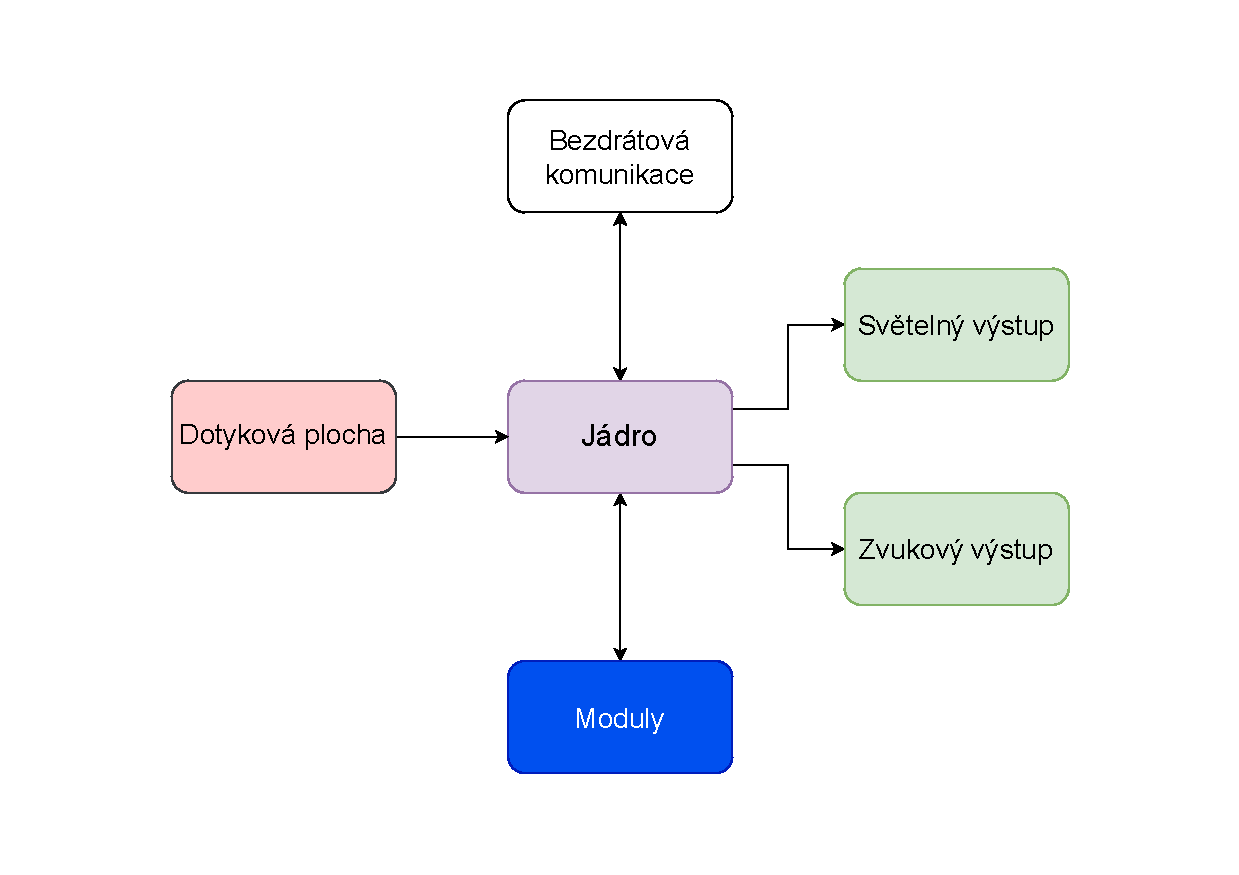
\includegraphics[width=\textwidth]{text/TeoretickyUvod/AplikaceHernichZarizeni/diagram/zanoreni_0.pdf}
    \caption{Úvodní blokové schéma zařízení}
    \label{fig:diagram_zanoreni_0}
\end{figure}

Co se~světelného výstupu týče, na~signalizaci různých stavů je~vhodné používat různé barvy světel.
% Jaký vzhled by~ale měl mít zdroj barevného světla na~podobném zařízení?
Jak je~vysvětleno v~následující podsekci \ref{VyuzitiTelefonu}, není potřebné suplovat grafický display, za~tímto účelem se~dá použít propojení s~telefonem.

Informace, kterou zařízení bude často poskytovat, je~čas a~směr, např. čas do~konce kola nebo směr k~dalšímu úkolu.
Podobné informace se~dají elegantně zobrazit na~kruhu.
%Protože má~být stanoviště pohodlně čitelné z~blízky i~viditelné z~větší vzdálenosti, je~tedy otázkou, zda použít jen jeden kruh, tak aby byl dostatečně viditelný, nebo jich použít více. %%TODO: otázka co~s~totu otázkou?
Je vhodné zobrazování rozdělit na~dva režimy, čtení na~dálku a~čtení na~blízko.
Pro čtení na~blízko je~cílem přímá interakce se~zařízením, např. u~zadávání hesla.
Čtení na~dálku je~naopak určeno pro předávání informací hráči, když právě přímo neinteraguje se~stanovištěm, např. který tým má~zrovna povolený přístup do~zařízení.
Proto je~vhodné mít kruhů více, aby bylo možné zobrazovat tyto informace na~různých kruzích, které mohou navíc být svému účelu přizpůsobeny.
Jeden kruh tak může svítit jen jedním směrem, aby ho~hráč viděl celý najednou pro blízkou interakci, zatímco druhý kruh může svítit do~všech stran, aby byl vidět z~co nejvíce míst.

Potřeba propojení s~telefonem nám omezuje možnosti co~se týče typu bezdrátové komunikace, protože telefony jsou většinou vybaveny Bluetooth a~WiFi.
Také se~v~telefonech rozšiřuje NFC, to~je však pro tuto aplikaci z~důvodu krátkého dosahu nevhodné.

Posledním systémem, který je~třeba zmínit, je~zvukový výstup.
Protože většinou stačí jen jednoduchá zvuková odezva, není potřeba plnohodnotný zvukový systém.
Pro hry, které budou potřebovat přehrávat libovolnou nahrávku, může být použit samostatný zvukový modul, případně je~možnost nahrávku přehrát přes uživatelův telefon.
V~základním zařízení je~proto potřeba jen jednoduchý bzučák, sloužící například jako odezva na~kliknutí.
Můžeme tedy upravit předchozí návrh.
Výsledkem je tak návrh, zobrazený na obr.~\ref{fig:diagram_zanoreni_1}.
\begin{figure}[h]
    \centering
    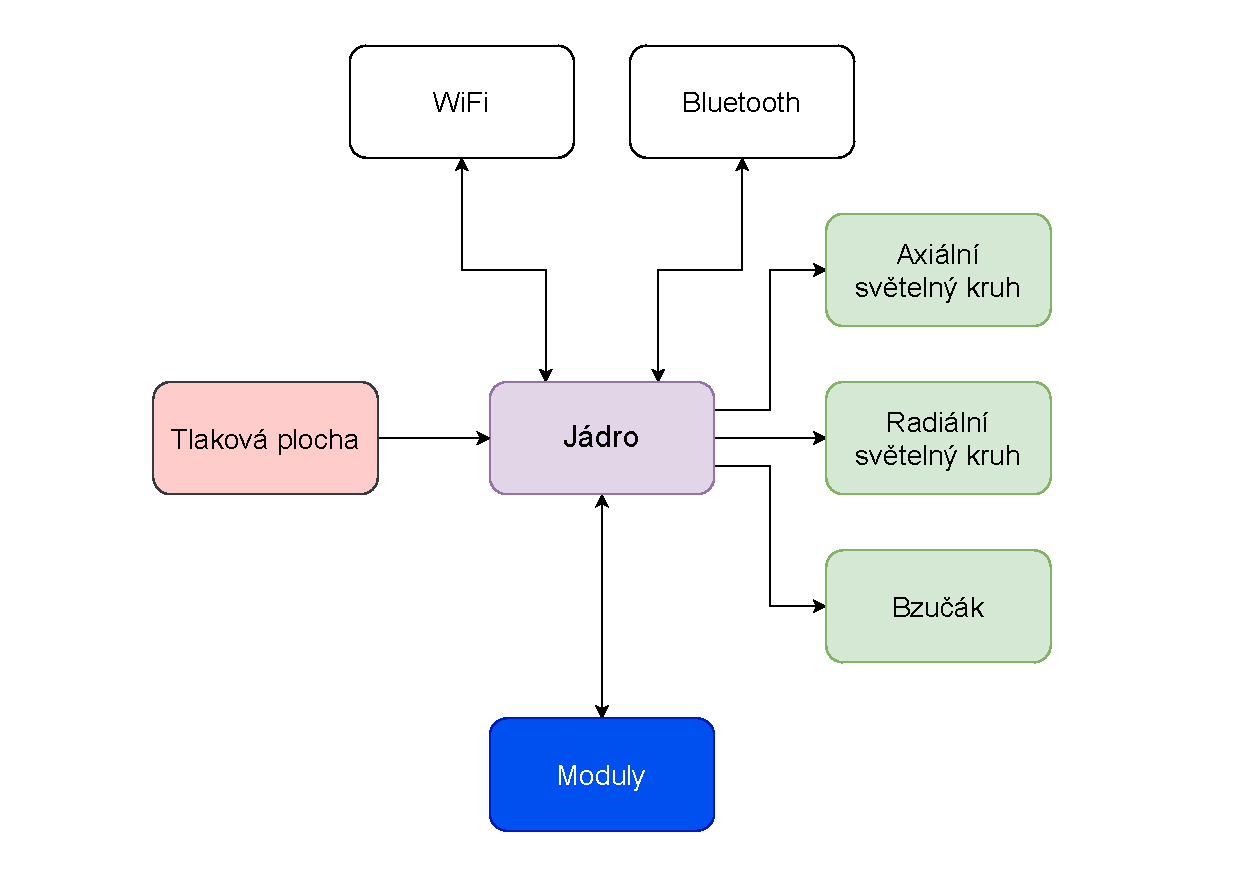
\includegraphics[width=\textwidth]{text/TeoretickyUvod/AplikaceHernichZarizeni/diagram/zanoreni_1.pdf}
    \caption{Základní blokové schéma zařízení}
    \label{fig:diagram_zanoreni_1}
\end{figure}

\section{Využití telefonu \label{VyuzitiTelefonu}}
Podstatný fakt je, že~prakticky všichni u~sebe dnes mají chytrý telefon, čehož mohu využít.
Nemá proto velký význam, aby statické nebo dynamické zařízení suplovalo funkce telefonu.
Např. grafický výstup typu display proto v~podobném zařízení není potřeba, a~v~tomto směru už~odvádí telefon naprosto dostatečnou práci.
Pokud by~tedy v~rámci hry bylo potřeba například předat hráči text nebo obrázek, může jej zařízení poslat uživateli na~telefon.
Telefon by~se tedy dal zařadit mezi dynamická zařízení.
Možnost propojení s~telefonem je~také velmi významná při nastavování hry.
Díky telefonu totiž zařízení nepotřebuje uživatelské rozhraní přizpůsobené k~nastavování, ale jednoduše se~nastaví z~telefonu.

Někdy by~se mohlo zdát, že~herní stanoviště vlastně ani není potřeba a~stačila by~mobilní aplikace.
Ale přestože je~telefon ve~hrách dobře využitelný, jsou aplikace, na~které jednoduše vhodný není.
Pokud má~hráč například ze~stanoviště získat fyzický objekt, telefon neposlouží.
Pro hráče ani organizátory také nemusí být zrovna komfortní před hrou zařizovat, aby měli všichni nainstalovaný správný software.
% Telefon také není například na~stanovišti v~lese dobře viditelný.
V~neposlední řadě jde také o~jistý ,,wow efekt'', který běžné zařízení jako mobil nebo třeba tablet neposkytne. %%TODO: tohle chce nějak přeformulovat


% \section{Základní řídící jednotka}
% % Z~toho plyne otázka, jaká funkcionalita je potřebná v~základním zařízení?
% Asi žádný systém, se kterým hráč přímo interaguje, není nutný v~každé hře.
% Jde tedy o~to vybrat takové systémy, které svými nároky nepřevýší užitečnost při hrách.
% Ze zkušeností považujeme za nejzákladnější systém nějaký světelný výstup, ten dokáže většinu her velmi příjemně ozvláštnit.
% Většinou je nezbytný i~uživatelský vstup, na což většinou stačí obyčejná tlačítka.
% Problém je ale určit jaké a~kolik jich bude potřeba.
% Některé hry vyžadují třeba jen jedno, ale takové, aby se do něj dalo co nejpohodlněji praštit v~běhu, protože je zrovna cílem ke stanovišti co nejrychleji doběhnout.
% Jiná hra může vyžadovat tlačítek víc, ale už není potřeba, aby byly tak velké, protože hráč při jejich používání nebude tak akční, ale bude třeba zadávat výsledek logického úkolu.
% Univerzálnější je tedy nepoužívat tlačítka, ale nějaký systém, který se dá softwarově přizpůsobit.
% Příkladem může být dotyková plocha, která se dá softwarově rozdělit na různé oblasti sloužící jako tlačítka a~i~během hry se tak dá počet tlačítek měnit.
% Další důležitou vlastností je možnost komunikace s~ostatními zařízeními, která do hry přináší novou možnost jak stanoviště propojit a~také pohodlnou metodu jak stanoviště nastavit přes telefon.
% V~neposlední řadě je potřeba zvukový výstup, který může být použit např. jako potvrzení zadaného hesla.

% Z~toho nám tedy plyne diagram \ref{fig:diagram_zanoreni_0}.
% \begin{figure}[h]
%     \centering
%     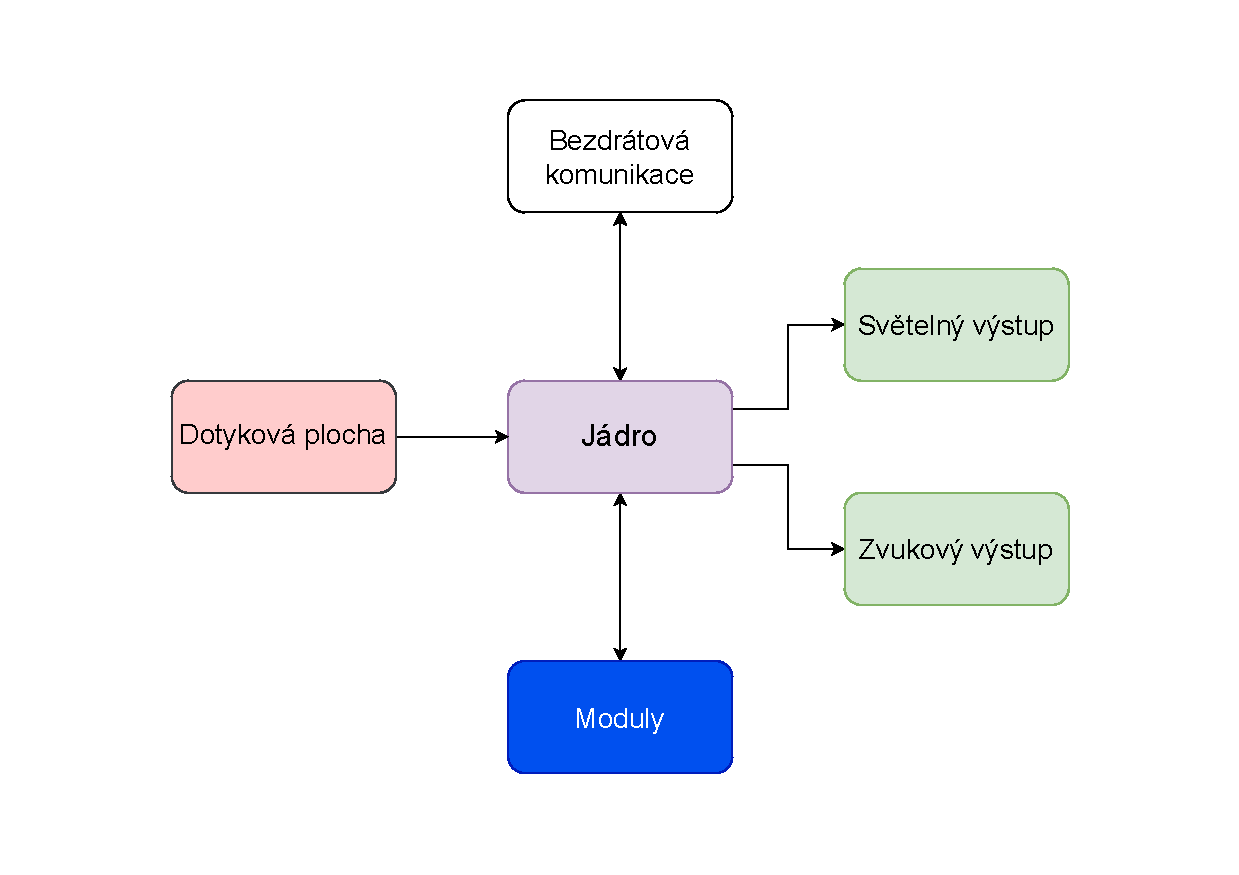
\includegraphics[width=0.65\textwidth]{text/TeoretickyUvod/AplikaceHernichZarizeni/diagram/zanoreni_0.pdf}
%     \caption{Úvodní blokové schéma zařízení}
%     \label{fig:diagram_zanoreni_0}
% \end{figure}

% \newpage

Co se~světelného výstupu týče, na~signalizaci různých stavů je~vhodné používat různé barvy světel.
% Jaký vzhled by~ale měl mít zdroj barevného světla na~podobném zařízení?
Jak je~uvedeno výše, není potřebné suplovat grafický display, za~tímto účelem se~dá použít propojení s~telefonem.
Informace, kterou by~zařízení mohlo často poskytovat je~čas a~směr, např. čas do~konce kola nebo směr k~dalšímu úkolu.
Podobné informace se~dají elegantně zobrazit na~kruhu.
Protože má~být stanoviště viditelné i~z~větší vzdálenosti, je~tedy otázkou, zda použít jen jeden kruh, tak aby byl dostatečně viditelný, nebo jich použít více. %%TODO: otázka co~s~totu otázkou?
Zobrazování pracuje ve~dvou režimech, čtení na~dálku a~čtení na~blízko.
Pro čtení na~blízko je~cílem přímá interakce se~zařízením např. už~zmiňované zadávání hesla.
Čtení na~dálku je~naopak určeno pro předávání informací hráči, když právě přímo neinteraguje se~stanovištěm, např. který tým má~zrovna povolený přístup.
Proto je~vhodné mít kruhů více, aby bylo možné zobrazovat tyto informace na~různých kruzích, které mohou navíc být svému účelu přizpůsobeny.
Jeden kruh tak může svítit jen jedním směrem, aby ho~hráč viděl celý najednou pro blízkou interakci, zatímco druhý kruh může svítit do~všech stran, aby byl vidět z~co~nejvíce míst.

Potřeba propojení s~telefonem nám omezuje možnosti co~se týče bezdrátové komunikace, protože telefony jsou většinou vybaveny Bluetooth a~WiFi.
Také se~v~telefonech rozšiřuje NFC, to~je však pro tuto aplikaci z~důvodu krátkého dosahu nevhodné.

Posledním systémem, který je~potřeba, je~zvukový výstup.
Protože většinou stačí jen jednoduchá zvuková odezva, není potřeba plnohodnotný zvukový systém.
Pro hry, které budou potřebovat přehrávat nějakou nahrávku, bude samostatný zvukový modul, případně je~možnost nahrávku přehrát přes uživatelův telefon.
V~základním zařízení je~proto potřeba jen jednoduchý bzučák, například jako odezva na~kliknutí.

Můžeme tedy diagram upravit na~\ref{fig:diagram_zanoreni_1}.
\begin{figure}[h]
    \centering
    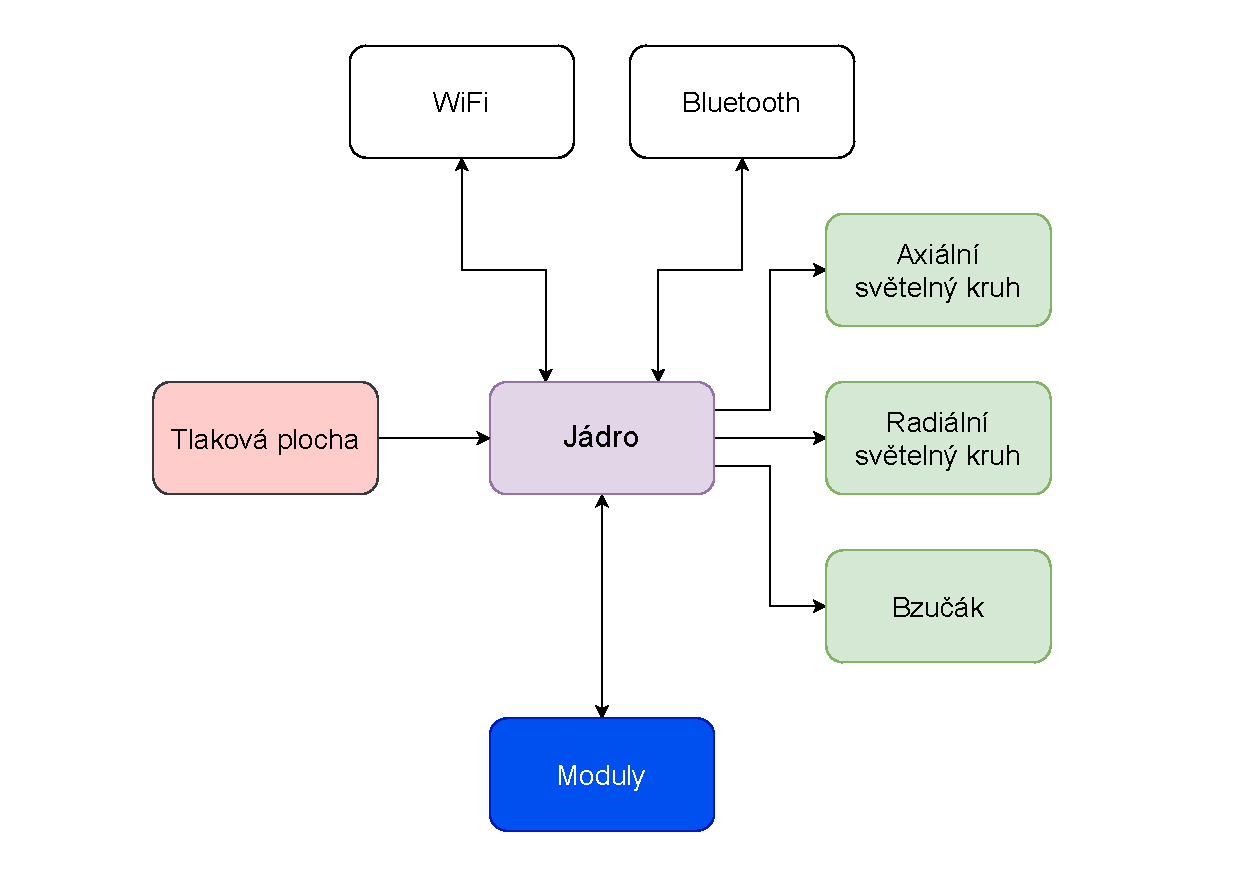
\includegraphics[width=0.65\textwidth]{text/TeoretickyUvod/AplikaceHernichZarizeni/diagram/zanoreni_1.pdf}
    \caption{Základní blokové schéma zařízení}
    \label{fig:diagram_zanoreni_1}
\end{figure}

Celé zařízení by~také mělo být alespoň částečně voděodolné, aby se~dalo použít třeba i~za~deště.

\vspace{-10mm}
\section{Moduly}
Základní řídící jednotka je~tedy schopná poskytnout základní funkce, které jsou potřeba pro většinu her.
Některé hry ale mohou vyžadovat nějakou specifickou funkci, kterou základní zařízení nedokáže poskytnout.
Proto je~vhodné, aby bylo možné k~základnímu zařízení připojit externí moduly, bez kterých by~se konkrétní hry neobešly.

\subsection{Modul dvířka}
Asi nejzákladnější modul jsou dvířka.
Dvířka přidávají uzamykatelné přihrádky.
Do stanoviště se~tak dá~uzamknout předmět potřebný ke~splnění úkolu, který hráči získají například po~zadání hesla nebo vyřešení zadaného úkolu.
Přihrádky pak mohou sloužit pro více týmů nebo třeba uchovávat více objektů do~různých částí hry.

Pro jednoduchost jsou dvířka zamykána magneticky.
Vrátka jsou uchycena \\ na~kloubu ve~své horní části a~v~dolní části se~nachází magnet.
Pod dnem přihrádky se~pak nachází servomotor vybavený druhým magnetem, který tak může dvířka přitáhnout nebo odpudit.
Toto řešení neposkytuje bezpečné uzamčení přihrádky, vrátka se~dají vypáčit někdy i~nehtem, ale pro účely her je~to dostačující řešení.
Aby bylo možné ověřit, zda se~vrátka dovřela, je~vedle serva i~spínač, který se~sepne při dovření vrátek.
Z~tohoto řešení vyplynula další možnost jak modul dvířek využít.
Vrátka se~při odemčení pootevřou, a~protože jsou v~tu chvíli jen odpuzována magnetem, je~možné je~stlačit zpět a~sepnout tak spínač.
Tento fakt se~ukázal být užitečný, protože tak vznikla velká pohodlná tlačítka.
Struktura tohoto modulu je~vidět na~diagramu \ref{fig:diagram_dvirka} ve~verzi se~čtyřmi přihrádkami.

\begin{figure}[h]
    \centering
    \includegraphics[width=\textwidth]{text/TeoretickyUvod/AplikaceHernichZarizeni/diagram/Dvirka.drawio.pdf}
    \caption{Blokové schéma modulu dvířka}
    \label{fig:diagram_dvirka}
\end{figure}
 
Jednoduchá hra, která vyžaduje modul dvířka, je~např. hra Maják. %%TODO: vymyslet lepčí název tohle se~ mi~moc nepozdává (je to~název z~her od~Petra na~první lucerný v~roce 2021)
V~této hře jsou hráči rozděleni do~týmů a~každý tým má~svou barvu, od~které je~odvozena konkrétní přihrádka. 
Týmy mají za~úkol získat co~nejvíc sad kartiček.
Na hřišti je~několik automatických stanovišť s~modulem dvířka a~v~každém z~nich je~nějaký typ kartičky.
Každé stanoviště během hry umožňuje přístup vždy právě jednomu z~týmů, který v~pravidelném intervalu mění, a~čas do~změny reprezentuje na~jednom z~kruhů.
Při startu hry si~každé stanoviště náhodně vybere tým, kterým začne, a~následně se~už drží konstantního pořadí.
Když někdo dorazí ke~stanovišti ve~chvíli, kdy je~stanoviště zpřístupněné jeho týmu, a~klepne na~tlakovou plochu, stanoviště mu~vydá kartičku.
Stanoviště se~týmu zpřístupní jen v~čase daného týmu a~navíc jen jednou za~kolo.
Hráčům cíleně není představen celý mechanizmus výdeje kartiček, je~jim řečeno jen, že~se přihrádka otevírá klepnutím do~tlakové plochy a~že je~zajímají jen kartičky jejich barvy. 
Tým tedy musí spolupracovat nejprve na~odhalení mechanizmu a~následně myslet jak zvítězit.

Podobná hra se~buď dá~hrát samostatně nebo může jít například jen o~metodu, jak získávat suroviny v~nějaké komplexnější hře.

\subsection{Zvukový modul}
Další plánovaný modul, který se~dá připojit, je~zvukový modul.
Hra, která vyžaduje zvukový modul, je~například hra s~názvem Ticho.
Tato hra vyžaduje zároveň i~modul dvířka.
V~této hře stanoviště sleduje intenzitu zvuku v~okolí a~v~momentě, kdy hluk klesne pod stanovenou úroveň, stanoviště otevře dvířka. 
% Ucastnikum není ovládání představeno a~musí tak na~něj přijít samy.
Stanoviště je~hráčům představeno jako "magická krabička"\- za~čárou, ke~které se~nesmí proplížit, ale můžou ji~ovlivnit z~dálky.
Úkolem hráčů tak je~přijít na~to, jak krabička funguje a~jak ji~přesvědčí, aby se~otevřela.

V~rámci zvukového modulu je~i~možnost nahrávku přehrát.
Tato část zvukového modulu umožňuje intenzivnější vtažení hráče do~hry s~příběhem.
Může jít například o~únikovou hru, při které se~hráč ocitne v~oblasti neznámého bludiště a~jeho úkolem je~najít cestu ven.
Při hledání může narazit na~různá stanoviště, která mu~nejprve přehrají nějakou část příběhu a~následně mu~dají úkol nebo radu jak postupovat dál.

% \subsection{Komunikační modul \label{sec:KomunikacniModul}}
% Podstatným modulem je~také komunikační modul, který umožňuje připojení k~mobilní síti a~tím i~komunikaci s~ostatními zařízeními na~velkou vzdálenost.
% Tento modul je~potřebný například pro hru Boj o kopce.

% V~této hře se~na hřišti o~velké rozloze nachází několik automatických stanovišť.
% Hráči jsou rozděleni do~týmů a~každý tým má~svou barvu a~své tlačítko na~stanovišti označené barvou týmu.
% V~hře je~hlavním cílem získávat body pro svůj tým ovládnutím a~udržením stanovišť na~rozsáhlém hřišti. 
% Axiální světelný kruh zobrazuje rozdělení tlakové plochy na~jednotlivá tlačítka týmů podle jejich barvy.
% Zabrání stanoviště pak mohou hráči provést stiskem příslušného tlačítka. 
% Získávání bodů se~odehrává dvěma způsoby, ovládnutím stanoviště a~následným držením stanoviště pod kontrolou. 
% Týmy mohou přebírat stanoviště od~soupeřů, což přidává hře strategický rozměr. 
% Výhodou je~kontrolovat více stanovišť najednou, což umožňuje rychlejší získávání bodů a~zvyšuje šanci na~vítězství.
% Komunikační modul je~tu potřebný pro vyhodnocování hry.
% Stanoviště totiž musí být schopné komunikovat s~centrálním serverem, který vyhodnocuje hru a~zobrazuje její průběh.
% Tato hra je~původně navržena pro airsoftové hráče na~hřiště v~Mokrá-Horákov o~rozloze \(6.7\-ha\) \cite{MokraHorakov}.
% V~takovém prostředí tedy komunikace pomocí WiFi či~Bluetooth nedostačuje, protože stanoviště mohou být i~několik set metrů od~sebe.

% \subsection{Výběr bezdrátové komunikace dlouhého dosahu \label{sec:TypVzdaleneKomunikace}}
% Pro komunikaci na~vzdálenosti v~řádu jednotek kilometrů se~nabízí asi jen dvě základní možnosti, LoRa a~mobilní síť.
% Ještě počátkem roku 2023 by~byla i~třetí možnost, Sigfox, ale jeho síť byla v~ČR vypnuta \cite{SigfoxKonci}.

% LoRa je~technologie určená pro komunikaci na~dlouhé vzdálenosti s~malou spotřebou a~datovou propustností.
% Pracuje v~bezlicenčním pásmu a~není tedy třeba platit za~provoz.
% Její dosah je~i~v~zastavěné oblasti v~řádu kilometrů \cite{LoRaSEMTECH}, a~za ideálních podmínek na~přímou viditelnost i~přes sto kilometrů \cite{LoRaEMAN}. 
% Nevýhoda LoRy je~ale malá datová propustnost ještě snížená omezením času provozu na~\(1\-\%\)\cite{LoRaEMAN}.

% Mobilní síť má~v~porovnání s~LoRou výrazně větší datovou propustnost, ale na~druhou stranu je~třeba platit za~provoz a~je méně energeticky úsporná.
% Například \\NB-IoT je~energeticky asi o~třetinu náročnější než LoRa.
% Přesto je~dostatečně úsporná, aby bylo zařízení, které tuto technologii využívá, schopno běžet na~baterii přes deset let \cite{LoRaVSNB-IoT}.
% Energetická náročnost tedy není problém a~vyšší datová propustnost společně s~připojením na~internet je~významnější výhoda než bezplatný provoz u~LoRy.
% Další výhodou LoRy by~mohla být nezávislost na~pokrytí mobilních sítí, ale vzhledem k~tomu, že~pokrytí NB-IoT sítě je~v~ČR údajně \(100\-\%\)\cite{NB-IoTPokryti}, není tento fakt důležitý. 

% \section{Dynamických zařízení}
% U některých her je~potřeba, aby měl hráč zařízení, které bude moci nosit s~sebou a~které mu~při hře bude sloužit jako identifikace nebo nástroj pro plnění úkolů.
Takové zařízení by~mělo být co~nejmenší a~co nejlehčí, aby hráče při hře nezdržovalo.
Navíc by~mělo být co~nejlevnější, aby tolik nevadilo, když jej některý hráč třeba ztratí, což se~přeci jen může stát.
Mimo to~toto zařízení musí být schopno zobrazit svůj stav a~převzít od~uživatele jednoduchý pokyn.

% Rozhodli jsme, že toto zařízení bude svůj stav zobrazovat pomocí pěti inteligentních RGB LED a jako vstup mu budou sloužit dvě tlačítka.
% Abychom nemuseli řešit napájení, má toto zařízení USB konektor a je určeno k napájení powerbankou.
% Toto zařízení jsme nazvali SemiSemafor a jeho vzhled je na obrázku \ref{fig:SemiSemafor}.

% \begin{figure}[h]
%     \centering
%     \includegraphics[width=0.8\textwidth]{text/TeoretickyUvod/AplikaceHernichZarizeni/img/1702085190411.jpg}
%     \caption{Zařízení SemiSemafor}
%     \label{fig:SemiSemafor}
% \end{figure}

% \subsection{Využití zařízení SemiSemafor}
% SemiSemafor je využitelný například ve hře s názvem Duchové.
% Nabiječa, artefakt, SemiSemafor = učastnická lucernička
% učastník dojde k nabiječce, nabije ce a u artefaktu předali energii
% lucerničky se samovibijí,
% když zmáčkneč tlačítko mužeš nabijet artefakt ale když uněj nejseš a lucernička se vybije dvakrát rychleji a odpuzuje duchy (svítí u toho bíle)
% duchová mají taky zařízení (Semiho) když drží tlačítko vybijí lucerničku i artefakty v okolí (nesvítí u toho)
% víc lidí muže naráz nabijet
% když duch chytí hráče, hráč si musí na pět minut ze hry, u nabíječky je respoun
% cílem je nabít všech tt artefaktů

% potenciálně by duchové mohli ke své činnosti potřebovat energiiž

%%% Vložení souboru 'text/vysledky' s popisem vysledků práce
% (rozdělte na více souborů či kapitol, pokud je vhodné)
\chapter{Návrh statického zařízení}
% Celé zařízení je~rozděleno na~základní jednotku a~případné moduly, které zajistí nové herní možnosti.
%~Například může jít o~připojení úložného prostoru nebo zvukového modulu, který poskytne jak plnohodnotný zvukový výstup tak vstup.

%~\subsection{uživatelské požadavky}
Uživatelským požadavkem je~statické zařízení sloužící jako herní stanoviště.
Vyžaduje tedy mobilitu jen v~rámci transportu na~místo hry a~zpět, nikoliv v~rámci samotné hry.
Z~toho plynou požadavky na~velikost výsledného zařízení.

Zařízení bude mít dva světelné kruhy složené z~60 RGB LED.
Číslo 60~jsem zvolil, protože se~jedná o~dostatečně jemné dělení, aby se~daly dělat plynulé efekty.
Zároveň jde o~číslo, které koresponduje s~hodinovým ciferníkem a~stupnicí na~kompasu.
Jeden z~kruhů bude radiální a~druhý axiální.

Axiální kruh bude umístěn~na horní stranu zařízení a~bude sloužit primárně jako odezva pro hráče na~malou vzdálenost, např. při zadávání hesla.
Radiální kruh pak bude umístěn také v~horní části zařízení a~jeho účelem bude naopak signalizace na~delší vzdálenost.
Například může sloužit jako maják viditelný ve tmě i~na stovky metrů.


%TODO: dopsat a~vygenerovat ilustraci
Uvnitř axiálního světelného kruhu se~bude nacházet tzv. tlaková plocha. %\label{popisTlakovky1}
Jedná se~o~ovládací prvek podobný dotykové ploše s~tím rozdílem, že~je schopen měřit i~sílu, která na~něj působí.
% Tento prvek je~založen na~měření rezonanční frekvence snímacích LC~článků, nad kterými se~nachází tlaková plocha.
% Tlaková plocha je~vodivý objekt, ve~kterém se~cívkou LC~článku indukují vířivé proudy a~následně se~jimi indukují proudy zpět v~cívce LC~článku.
% Tím plocha ovlivňuje indukčnost cívky a~tedy i~rezonanční frekvenci LC~článku.
% Ovlivnění indukčnosti je~závislé na~vzdálenosti plochy od~cívky a~tedy i~na~síle, která na~plochu působí.
% Velikost síly, která na~plochu působí, totiž ovlivňuje její průhyb a~tedy i~vzdálenost od~cívky.
% Díky velkému rozlišení použitého čipu LDC1614 \cite{LDC1614} (28 bitů) je~možné měřit změny vzdálenosti v~řádu jednotek mikrometrů \cite{LDC1614LinearPositionSensing}.
% Tato metoda je~tedy schopna měřit vzdálenost plochy od~jednotlivých cívek, které jsou čtyři, a~plochu tak snímají na~čtyřech místech.
% Následně je~z~těchto hodnot možno dopočítat, jak je~plocha nakloněna a~tím určit, kde se~jí uživatel dotýká.
%~Protože je~zároveň možné určit i~sílu jakou uživatel při dotyku vyvinul, dostal tento systém jméno tlaková plocha. %~silová by~bývalo přesnější ale nějak mi~to nejde přes pysky

Aby bylo stanoviště reálně použitelné při hře, musí celou hru vydržet na~baterii.
Není ojedinělé, aby měla bojovka čtyři i~pět hodin bez přestávky.
Plus je~nutná časová rezerva a~čas na~nastavování.
Čas, který zařízení zvládne běžet z~baterie, silně závisí na~činnosti, ale nebylo by~zrovna ideální, kdyby baterie byla výrazně omezujícím faktorem.
Výdrž na~jedno nabití by~tedy měla být alespoň šest hodin.

Vzhledem k~plánu připojovat moduly je~nutné navrhnout mechanizmus připojení.
Bylo by~ideální, kdyby si~mohl uživatel říct, co~bude hrát za~hru, a~podle toho si~sám připojil moduly, které potřebuje.
Tomuto určitě nechci bránit, ale přímo to~podporovat nese~řadu problémů, jak ze~strany konektoru a~mechaniky, tak ze~strany softwaru.
Konektor by~totiž musel být ideálně beznástrojově rozpojitelný a~opětovně spojitelný a~přitom dostatečně pevný, aby se~zařízení mechanicky chovalo jako jeden celek.
Takový konektor je~ale poměrně složité vyrobit, tak aby byl spolehlivý, a~tak jde v~tuto chvíli jen o~možnost dalšího vývoje.
Ze softwarového pohledu jde pak o~problém, jak detekovat konkrétní modul a~hlavně o~otázku, jak se~chovat k~modulům, které jsou potenciálně záměnné.

% Dejme tomu, že~máme modul klávesnici a~modul dvířka.
% Dvířka jsou původně navržena primárně jako úložný prostor, díky detekci zavření je~lze ale použít i~jako pohodlná tlačítka a~v~některých hrách se~proto používají jen jako tlačítka.
% Potenciální modul klávesnice je~ovšem jen suma tlačítek.
% Při vytváření konkrétní hry na~míru modulům, které herní návrhář má~zrovna k~dispozici, je~tento problém nepodstatný, protože sám návrhář rozhodne, co~má jak být.
% Ale ve~chvíli, kdy jde o~hru navrženou pro jinou kombinaci modulů, nastává problém jak rozhodnout, zda se~dají dvířka použít místo klávesnice nebo ne~a~naopak.
% Abych se~všem těmto problémům alespoň prozatím vyhnul, rozhodl jsme se, že~doplnění či~výměna modulu půjde jen při servisním zásahu.
% Problém záměny modulů tak budu řešit tím, že~každá hra bude vytvořena jen pro konkrétní sadu modulů.

V~řadě případů je~užitečné mít možnost zvukové zpětné vazby.
Ideální by~bylo moci přehrávat libovolnou nahrávku, většinou ale stačí jednoduchý tón, řekněme jako potvrzení zadaného hesla.
Pro možnost přehrávání plnohodnotného zvuku bude proto sloužit samostatný modul a~v~základní jednotce, postačí jednoduchá sirénka.

Z~požadavků mi~vyplynulo zařízení, jehož možný vzhled je~nastíněn na~obrázku \ref{fig:AHS-nacrt}.
\begin{figure}[h]
    \centering
    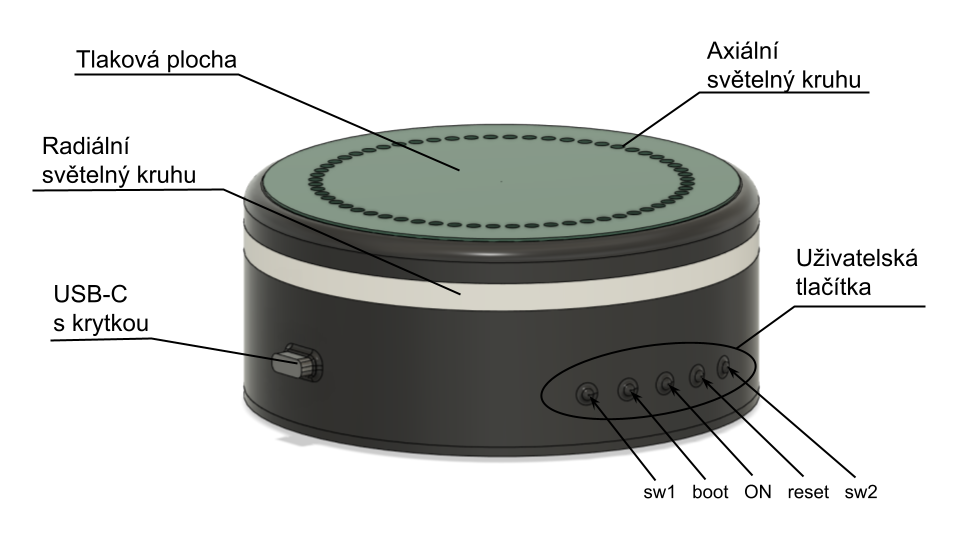
\includegraphics[width=\textwidth]{text/PraktickaCast/img/AHS-nacrt.png}
    \caption{Návrh vzhledu zařízení}
    \label{fig:AHS-nacrt}
\end{figure}

\newpage
\section{Elektronické systémy zařízení}

Elektronika bude~rozdělena na~dvě samostatné DPS.
Pujde o~hlavní desku, na~které bude umístěna většina elektroniky a~o~desku s~hlavním uživatelským rozhraním (LED deska).
Kompletní schéma a~topologie DPS je~k~vidění v~přílohách (schéma je~k vidění v~příloze \ref{AHS-sch} a~DPS v~příloze \ref{AHS-pcb}).

%~Původně jsem uvažoval ještě třetí desku, se~základním uživatelským rozhraním (mini~UI) pro usnadnění zajištění jisté míry voděodolnosti, ale nakonec jsem se~rozhodl spojit ji~s~hlavní deskou.

\subsection{LED deska}
Na LED desce budou umístěny oba světelné kruhy a~elektronika pro snímání tlakové plochy, tedy LDC1614 \cite{LDC1614} a~jeho snímací LC~články.
Právě snímaní tlakové plochy je~jeden z~hlavních důvodů oddělení této elektroniky na~samostatnou desku, zabere totiž na DPS velkou plochu.

Na LED desce se~tedy nachází:
\begin{itemize}
    \item Axiální LED kruh z~60 RGB LED WS2812B v~pouzdře \(3,5\)\;x\;\(2,8~mm\)
    \item Radiální LED kruh z~60 RGB LED WS2812B v~pouzdře \(3,5\)\;x\;\(2,8~mm\)
    \item LDC1614 se~čtyřmi snímacími LC~články pro snímání tlakové plochy 
    \item konektor na~propojení s~hlavní deskou
\end{itemize}

% Čip LDC1614 \cite{LDC1614} lze zaměnit za~LDC1314 \cite{LDC1314}, tyto čipy se~liší vlastně jen šířkou výstupního registru.
% Dalo by~se~tedy čekat snížení citlivosti při použití verze čipu LDC1314, není to~ale úplně pravda.
% Uživatel si~u~LDC1314 ale musí zvolit kompromis mezi rozsahem měření a~jeho citlivostí.
% Nastavení se~navíc dá~jednoduše měnit za~chodu, takže by~LDC1314 znamenalo nanejvýš trochu složitější program ale ne~nutně ztrátu citlivosti nebo rozsahu. 

\newpage
\subsection{Hlavní deska}

Řídícím mikrokontrolérem AHS bude ESP32-S3 (výběr je~rozebrán v~podsekci \ref{subs:vybermikrokontroléru}).
Na hlavní desce bude spolu s~mikrokontrolérem také zdroj poskytující správné napájení všech systémů zařízení.
Hlavní deska bude tedy zprostředkovávat několik napěťových větví.
V~neposlední řadě se zde bude nacházet základní uživatelské rozhraní v~podobě několika tlačítek, jednoduché RGB LED a sirénky.

Zdroj AHS je~tvořen dvěma LiIon články 18650 v~paralelním uspořádání.
Dva články volím, abych zajistil dostatečnou výdrž baterie a~abych využil volné místo v~zařízení.
Paralelní uspořádání jsem volil, aby nebyl nutný balancer při nabíjení, a~tedy abych zjednodušil zařízení.

Elektronika řeší i~nabíjení baterie, současně s~čímž realizuje i~ochranu proti podbití a~případnému přebití.
Aby nebylo možné softwarově baterii podvybít, má~AHS už~zmíněnou ochranu proti podvybití řešenou čistě hardwarově.
Tato ochrana tak celé zařízení vypne v~případě, že~dojde k~vybití baterie pod napětí \(2,8~V\).
Pochopitelně, software by~měl vybitou baterii zaznamenat mnohem dřív a~chovat se~podle toho, např. neumožnit spustit hru napětí na baterii \(3,0~V\).

Abych vyhověl napěťovým požadavkům všech použitých systémů, jsou na~hlavní desce tři různá napájecí napětí, která se~dál dělí do~šesti napájecích větví.
\begin{itemize}
    \item VCC, napětí baterie sloužící jako zdroj pro ostatní napájecí větve a~pro napájení komunikačního modulu. 
    \item Napětí \(3,3~V\) na~napájení logické části celého základního zařízení.
    \item Napětí \(5,0~V\) pro LED desku a~externí moduly a~napájení z~USB
    \begin{itemize}
        \item V-USB, z~USB-C konektoru pro nabíjení a~programování
        \item 5V-A, pro napájení modulu na~modulovém konektoru
        \item 5V-B, pro napájení LED kruhů
        \item 5V, jakožto zdroj pro větvě 5V-A a~5V-B 
    \end{itemize}
\end{itemize}
Napětí větví \(3,3~V\) je~tvořeno pomocí LDO.
Na vytvoření větve 5V~je ale potřeba spínaný zdroj.
Především proto, že napětí baterie, ze~které se~tato větev napájí, má~nižší napětí a~je jej tedy třeba transformovat na~napětí vyšší.
Navíc tento zdroj poskytuje do~systému proudy o~hodnotě až pět ampér a~bylo by~tedy vhodné použít spínaný zdroj i~v~případě vyššího vstupního napětí.
LDO by tak mělo malou efektivitu převodu a~především by~vytvářel nemalé množství odpadního tepla, se kterým by se zařízení muselo vypořádat.

Na hlavní desce je~také řada konektorů sloužících pro připojení ostatních systémů.
Jde o~konektory na:
\begin{itemize}
    \item propojení s~LED deskou,                % samostatný objekt
    \item externí moduly,                        % samostatný objekt
    \item USB-C (nabíjení a~programování AHS),   % externě definovaný objekt
    \item programátor,                           % samostatný objekt
    \item slot pro SD~kartu.
\end{itemize}
Do~konektorů by se také dal zařadit držák na~dva LiIon články 18650.

\subsection{Výběr mikrokontroléru \label{subs:vybermikrokontroléru}}
Požadavky na výbavu mikrokontroléru jsou:
\begin{itemize}
    \item WiFi,
    \item Bluetooth,
    \item alespoň 2~UARTy,
    \item alespoň 22~GPIO pinů,
    \item I2C,
    \item dostatečný výpočetní výkon pro hladký chod interpretru JavaScriptu nebo Pythonu.
\end{itemize}

Porovnání některých dostupných možností je~provedeno v~tab. \ref{tab:vybermikrokontroléru}.
\begin{table}[h]
    % \hspace{-20mm}
    \small
    \begin{tabular}{|l|l|l|l|l|c|}
        % \hline
        % mikrokontrolér                  ~&~Jádro         &~Počet GPIO pinů    & Počet UARTů  ~&~Počet I2C &~Wi-Fi a~Bluetooth                \\ \hline
        \hline
        \makecell{Mikro-\\kontrolér}    & Jádro         &~\makecell{Počet\\GPIO pinů} &~\makecell{Počet\\UARTů} &~\makecell{Počet\\I2C} &~\makecell{Wi-Fi a\\Bluetooth} \\
        \hline
        ESP32        \cite{ESP32}       &~2x Xtensa LX6 &~34    ~            & 3            ~&~2         &~\textcolor{green}{\checkmark}    \\ \hline
        ESP32-S3     \cite{ESP32S3}     &~2x~Xtensa LX7 &~45    ~            & 3            ~&~2         &~\textcolor{green}{\checkmark}    \\ \hline
        ESP32-C3     \cite{ESP32C3}     &~1x~RISC-V     &~16-22              & 2             &~1         &~\textcolor{green}{\checkmark}    \\ \hline
        ESP32-C6     \cite{ESP32C6}     &~1x~RISC-V     &~34    ~            & 3            ~&~2         &~\textcolor{green}{\checkmark}    \\ \hline
        PIC32MZ-W1  ~\cite{PIC32MZ}     &~DS60001192    & 62    ~            & 3            ~&~2         &~\textcolor{green}{\checkmark}    \\ \hline

        \textcolor{red}{nRF7000      \cite{nRF7000}}      &~-             &~\textcolor{red}{13}& \textcolor{red}{0} &~\textcolor{red}{0}    & \textcolor{green}{\checkmark}    \\ \hline
        \textcolor{red}{RTL8710      \cite{RTL8710}}      &~ARM Cortex-M3 &~\textcolor{red}{17}& \textcolor{red}{1} &~3                     &~\textcolor{green}{\checkmark}    \\ \hline
        \textcolor{red}{RTL8721DM    \cite{RTL8721DM}}    & -            ~&~\textcolor{red}{17}& 3                  & 2                    ~&~\textcolor{green}{\checkmark}    \\ \hline
        \textcolor{red}{STM32WB55    \cite{STM32WB55}}    & ARM Cortex-M4 &~37    ~            & \textcolor{red}{1} &~2                     &~\textcolor{red}{$\times$}        \\ \hline
        \textcolor{red}{MSP430BT5190 \cite{MSP430BT5190}} &~-             &~32                 &~4                 ~&~4~                   ~&~\textcolor{red}{$\times$}        \\ \hline
    \end{tabular}
    \caption{Dostupné vyhovující mikrokontroléry}
    \label{tab:vybermikrokontroléru}
\end{table}

Abych nemusel návrh komplikovat anténou, použil jsem v~návrhu mikrokontrolér na~modulu, který má~anténu integrovanou, a~navíc integruje i~flash paměť. 
Protože už~tyto moduly interně používají některé GPIO, klesne množství, které mohu využít.

\begin{table}[h]
    \centering
    \begin{tabular}{|l|l|l|l|l|}
        \hline
        mikrokontrolér                  & Počet GPIO pinů    & vyhovuje?                     \\ \hline
        ESP32-WROOM     \cite{ESP32}    & 26                 & \textcolor{green}{\checkmark} \\ \hline
        ESP32-S3-WROOM  \cite{ESP32S3}  & 36                 & \textcolor{green}{\checkmark} \\ \hline
        ESP32-C3-WROOM  \cite{ESP32C3}  & 15                 & \textcolor{red}{$\times$}     \\ \hline
        ESP32-C6-WROOM  \cite{ESP32C6}  & 23                 & \textcolor{green}{\checkmark} \\ \hline
        WFI32E01PC      \cite{PIC32MZ}  & 37                 & \textcolor{green}{\checkmark} \\ \hline
    \end{tabular}
    \caption{Moduly s~mikrokontroléry}
    \label{tab:ModulySmikrokontroléry}
\end{table}

Jedním z~požadavků na~zařízení je~dostatečný výpočetní výkon pro hladký chod interpretu JavaScriptu nebo Pythonu.
Výpočetní výkon se~porovnává poněkud složitěji, protože se~nejedná tak úplně o~jeden parametr.
V~tomto případě je~ale vhodné prozkoumat i~dostupnost interpretu pro daný mikrokontrolér.
Pro ESP32 a~ESP32-S3 je~dostupný JavaScriptový interpret Jaculus \cite{Jaculus} i~interpret jazyka Python MicroPython \cite{MicroPythonESP32S3} \cite{MicroPythonESP32}.
Pro PIC32MZ-W1 a~ESP32-C6 je~dostupný pouze interpret jazyka Python MicroPython \cite{MicroPythonPIC32MZ-W1} \cite{MicroPythonESP32C6}. %interpret JavaScriptu jsem však nenašel.
ESP32 a~ESP32-S3 tak poskytuje výhodu v~možnosti volby skriptovacího jazyka.
ESP32-S3 má~oproti starší verzi ESP32 výkonnější jádro a~interpret JavaScriptu, resp. Pythonu, na~něm tak běží o~něco plynuleji.

Další výhodou ESP32-S3 oproti PIC32MZ-W1 je~jeho cena, která se~pohybuje okolo 4~USD \cite{JSC-ESP32-S3}.
Zatímco PIC32MZ-W1 je~u~JLCPCB za~13.65~USD \cite{JSC-WFI32}.
Navíc u~firmy JLCPCB, kde plánuji elektroniku vyrábět, sice je~PIC32MZ-W1 v~nabídce, ale není na~skladě \cite{JSC-WFI32}, zatímco u~ESP32-S3 bylo v~době návrhu dostupných hned 19~variant \cite{JSC-ESP32-S3}.

V~mém případě má~ESP32-S3 ještě jednu podstatnou výhodu, a~tou je~fakt, že~s~rodinou mikrokontrolérů ESP32 mám dlouholeté zkušenosti.
Z~těchto důvodů jsem se~rozhodl pro ESP32-S3.

\subsection{Tlaková plocha \label{popisTlakovky2}}
Tlaková plocha je~založena na~měření indukčnosti čtyř cívek.
Tyto cívky jsou použity spolu s~paralelně řazeným kondenzátorem, aby dohromady tvořily rezonanční LC~článek.
Zároveň jsou cívky vytvořeny jako reliéf v~mědi DPS, aby jimi vytvořené magnetické pole sahalo mimo ně~a~dalo se~tak použít pro ovlivnění jejich vlastností.

V~objektu vloženém do~proměnného magnetického pole vytvářeného cívkou se~vytváří vířivé proudy, které následně tvoří magnetické pole ve~směru opačném k~poli vytvořenému cívkou.
Magnetické pole vzniklé z~vířivých proudů tak indukuje další proudy zpět v~cívce, čímž snižuje její zdánlivou indukčnost.
Ve výsledku tak objekt v~magnetickém poli cívky ovlivňuje její indukčnost.
Velikost indukovaných vířivých proudů a~tedy i~míra ovlivnění indukčnosti cívky, je~závislá na~vodivosti daného objektu (terčíku), na~jeho rozměrech a~na jeho poloze vůči cívce.
V~případě pohybu terčíku, pouze ve~směru kolmém k~ploše DPS s~vytvořenou cívkou, se~tak převádí vzdálenost terčíku a~DPS na~indukčnost cívky.
Vizualizace popsaného mechanizmu sa nachází na obr. \ref{fig:pryncip-LDC}.

\begin{figure}[h!]
    \centering
    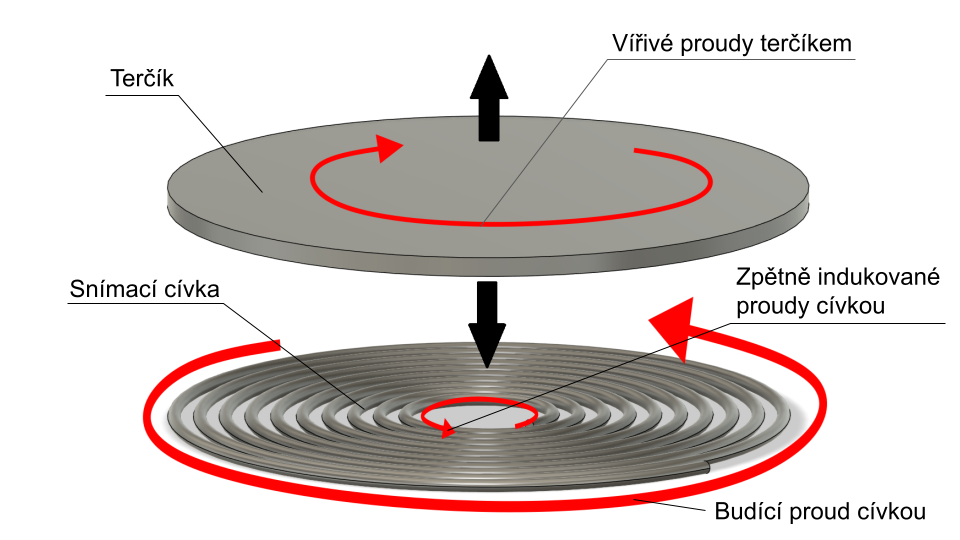
\includegraphics[width=\textwidth]{text/PraktickaCast/img/civka_tercik_ilustrace.png}
    \caption{Princip převodu vzdálenosti na~indukčnost}
    \label{fig:pryncip-LDC}
\end{figure}

Protože pro indukci vířivých proudů v~terčíku musí být magnetické pole cívky proměnné, musí být i~proud cívkou proměnný a~tedy i~napětí na~celém LC~článku.
V~případě použití čipu LDC1614 je~tedy LC~článek chvíli buzen nastaveným proudem, dokud nedosáhne nastavené napěťové amplitudy.
Následně přejde do~stavu měření, ve~kterém změří rezonanční frekvenci LC~článku porovnáváním s referenčním oscilátorem.
LDC1614 má interní oscilátor s~frekvencí \(40\)~{\itshape MHz}, ale např. v~aplikacích náročných na~přesnost je~možné připojit oscilátor externí. 
V~případě využití více kanálů následně přepne na~další kanál a~opakuje stejný postup \cite{LDC1614}.

Princip tlakové plochy tedy spočívá ve~snímání vzdálenosti terčíku, se~kterým přichází do~kontaktu uživatel, čtyřmi snímacími cívkami na~LED desce.
Princip uspořádání je~zobrazen na~obrázku č.\ref{fig:nastin-tlakovky}.

Kromě katalogových listů čipu LDC1614 jsem vycházel i~z~informací uvedených v~aplikační poznámce firmy Texas Instruments \cite{LDC1614SensorDesign} a~ze skript předmětu Mikrosenzory a mikroelektromechanické systémy \cite{SkriptaMMS}

\begin{figure}[h!]
    \centering
    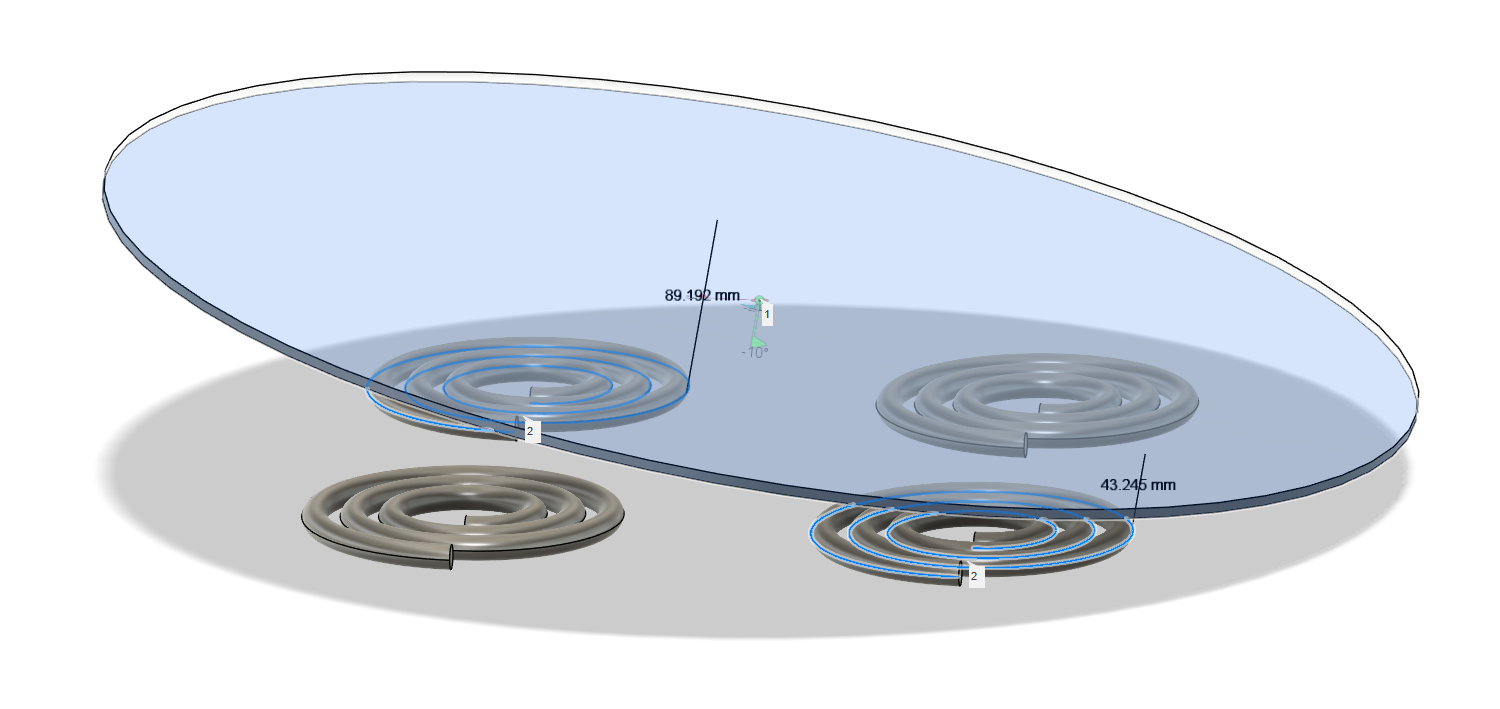
\includegraphics[width=\textwidth]{text/PraktickaCast/img/naklonena-tlakovka.png}
    \caption{Nástin principu snímání tlakové plochy}
    \label{fig:nastin-tlakovky}
\end{figure}

\subsection{Propojení hlavní desky a~LED desky}
Mezi hlavní deskou a~LED deskou je~třeba převést napájení a~několik signálů.
LED deska vyžaduje na~konektoru přítomnost dvou napájecích větví, \(5~V\) pro světelné kruhy a~\(3.3~V\) pro snímání tlakové plochy.
Protože do~RGB diod může téct proud až~\(5~A\) a~může být zároveň i~rychle spínaný, považuji za~rozumné oddělit napájecím větvím zem, abych omezil průnik rušení z~diod do~snímání tlakové plochy.
Oddělení je~tedy provedeno už~na konektoru hlavní desky a~už~v~kabelu jsou tedy větve vedeny samostatně.

Na samotné propojení jsem se~rozhodl použít FFC kabel s~roztečí \(0.5~mm\), pro jeho rozměry a~cenovou dostupnost.
Jedním vodičem takovéhoto kabelu lze vést proud maximálně \(0.4~A\) \cite{FFC-konektor}.
Protože ale potřebuji dodat proud až~\(5~A\), použiji \(13\) vodičů vedle sebe pro jednu cestu, jakožto nejmenší počet, který přenese~požadovaný proud v~rámci daných mezí.

Mimo napájení je~tímto propojením veden i~signál s~daty pro světelné kruhy a~I2C sběrnice se~signálem přerušení pro připojení čipu LDC1614 \cite{LDC1614}.
Výsledný počet vodičů v~kabelu je~tedy \(2 \cdot 13\) pro napájení, \(1\) pro data k~LED kruhům, dále \(2\) pro I2C, \(1\) pro signál přerušením a~nakonec \(2\) pro napájení snímání tlakové plochy.
Dohromady tedy kabel potřebuje \(32\) vodičů. 

Vzhledem k~počtu potřebných vodičů jsem se~rozhodl použít běžný FFC kabel se~40 kontakty s~tím, že~zbylé kontakty se~mohou hodit v~budoucnu.

\subsection{Modulový konektor \label{sec:ModulovyKonektor}}
Modulovým konektorem je~vedeno \(5~V\) jako napájení pro moduly a~komunikační sběrnice se~signálem přerušení pro komunikaci.

Nad volbou komunikační sběrnice jsem strávil značné množství času.
Původně jsem uvažoval o~využití RS485 jakožto odolné sběrnice, u~které by~v~případě potřeby nemusel být problém ani delší kabel.
RS485 má~ale nevýhodu v~tom, že~potřebuje dodatečný hardware, kterému bych se~hlavně na~modulech rád vyhnul.
Obdobný problém nastal u~CANu a~USB.
USB by~navíc mělo výhodu kompatibility s~velkým množstvím hotových zařízení.

V~první úvaze o~využití UARTu jsem jej zavrhl kvůli potenciální náročnosti na~přeposílání dat mezi moduly.
Při standardním použití bych totiž moduly řadil do~řetězu za~sebe.
Prvnímu modulu by~tak chodila data pro všechny ostatní moduly a~musel by~je přeposílat dál, což by~mohlo stát nezanedbatelné množství procesorového času.
%~TODO: nová linka, duvody, obhajoba

V~jisté chvíli jsem ale narazil na~nestandardní komunikaci pomocí UARTu implementované v~projektu Servio \cite{Servio}.
Tato implementace používá UART jako sběrnici.
Namísto standardního použití pro komunikace jeden-s-jedním tak může komunikovat jeden-s-více.
Na tomto řešení je~výhodné, že~nevyžaduje žádný dodatečný hardware a~prakticky každý dnešní mikrokontrolér je~možné k~této sběrnici velmi snadno připojit.

Ve srovnání s~RS485 je~sice mnohem méně odolná proti rušení, ale uvnitř zařízení nebude linka vedena na~příliš velkou vzdálenost.
Komunikace na~delším kabelu je~pak jednoduše nahraditelná bezdrátovou komunikací a~není tak potřebné, aby to~tato sběrnice v~základu podporovala.
% Navíc v~případě potřeby delšího kabelu je~možné navrhnout externí modul, který z~této sběrnice velmi jednoduše udělá RS485 pro externí využití.
% Alternativně by~se~pro komunikaci na~delším kabelu dalo použít USB, které je~společně s~nabíjením přivedeno na~USB-C.

Všechny moduly jsou připojeny na~jeden RX~pin AHS.
Proto musí firmware AHS zajistit, aby dva moduly nevysílaly současně.
Aby se~zabránilo možným zkratům, má~jako ochranu každý modul své piny UARTu připojeny přes rezistor \(180~\Omega\).
Pin~přerušení má na modulech naproti tomu jen schopnost signál přizemnit a~na straně hlavního zařízení je~dráha připojena přes rezistor k~napětí \(3,3~V\).
Abych alespoň trochu zvýšil odolnost linky proti rušení, přidám na~přijímací stranu pull-up rezistor.
Cílem je~zvýšení komunikačního proudu, aby se~případný proud vyvolaný rušením neprojevil.
V~neposlední řadě mají všechny piny na~konektoru ESD ochranu \cite{TPD4E02B04}.

\subsection{Konektor programátoru}
Zařízení se~dá jednoduše programovat přes USB-C, tento kanál je~ale možné softwarově narušit a~pro takové případy je~tu konektor na~programátor.
Jde o~šest plošek, na~které se~programátor připojuje pomocí pružinkových kontaktů.
Programátor sice obsahuje jen jednoduchou elektroniku, která by~mohla být i~přímo v~elektronice AHS, ale ve~většině případů by~byla zbytečná.
Ve chvíli, kdy by~byla potřeba, je~stejně nutná odborná obsluha a~pro tu~není problém použít externí programátor.

\subsection{USB-C}
USB-C je~použito pro nabíjení a~pohodlnější programování zařízení bez potřeby programátoru.

USB-C v~základu neposkytuje žádné napájecí napětí, protože je~navrženo k~obousměrnému provozu a může napájení jak poskytovat, tak spotřebovávat.
% Asi nejjednodušší zpusob jak požádat zdroj o~napájení je~dva rezistory s~hodnotou \(5.1~k\Omega\), přes které se~připojí signály \(CC1\) a~\(CC2\) k~zemi.
Asi nejjednodušší způsob jak požádat zdroj o~napájení, je~připojit dráhy {\it CC1} a~{\it CC2} k zemi přes rezistory o~hodnotě \(5.1~k\Omega\).
Takto zařízení dostane napětí \(5~V\) s~omezením proudu do~\(0.5~A\), tedy výkon \(2.5~W\).
V~tuto chvíli by~se~zařízení už~mohlo nabíjet, výkonem \(2.5~W\) by~se~ale nabíjelo velmi pomalu.
Proto jsem implementoval další systém, který má~za úkol zvýšit nabíjecí výkon a~tak zrychlit nabíjení.
Čip BQ25895M \cite{BQ25895} slouží primárně pro řízení nabíjení, ale zároveň se~stará o~komunikaci se~zdrojem a~zprostředkovává tak vyšší nabíjecí proud.
Velikost nabíjecího proudu se~navíc dá~v~případě potřeby nastavit přes I2C sběrnici z~ESP32-S3.

\subsection{Správa zapínání}
Zařízení je~vybaveno obvodem umožnujícím vypnutí jak uživatelské, tak programové a~v~případě hrozícího podbití i~automaticky.
Tento obvod zároveň kontroluje i~potenciální přebití baterie a~v~takovém případě odpojuje napájení nabíječky.

Původní verze správy zapínání je~vidět na~obr. \ref{fig:stary_PoverManager} (zapojení zapínacího tlačítka je~zjednodušeno, protože jeho zapojení je~složitější z~důvodu jeho čtení z~procesoru).

Na úvod popisu funkce je~vhodné říct, že~rezistor \(R_{5}\) slouží pro definici napětí na~\(G\) tranzistoru \(Q_{2}\) ve~chvíli vypnuté větve {\it 3V3} a~má~dostatečně velký odpor, aby se~při ostatních úvahách dal zanedbat.
Hlavní spínač je~PMOS tranzistor \(Q_{p1}\), který je~řízený NMOS tranzistory \(Q_{1}\) a~\(Q_{2}\).
Obvod \(U_{1}\) kontroluje stav baterie a~v~případě nízkého napětí na~dráze {\it Baterie} předpokládá, že~došlo k~limitnímu vybití baterie a~připojí na~vývod {\it OD}~(Over Discharge) \(0~V\) \cite{SL8261}.
To znamená zavřený tranzistor \(Q_{1}\), což znamená, že~se~rozepne i~tranzistor \(Q_{P1}\), protože se~jeho elektroda \(G\) vybije skrz rezistor \(R_{2}\).
Pokud je~baterie naopak nabita dostatečně, je~na vývod \(OD\)~obvodu \(U_{1}\) přivedeno jeho napájecí napětí \cite{SL8261}, v~našem případě tedy napětí baterie, které je~tak přivedeno na~\(G\) tranzistoru \(Q_{1}\).
Tranzistor \(Q_{1}\) je~tak otevřený, což znamená, že~zařízení má~povolení k~zapnutí. 
Když v~tuto chvíli dojde ke~stisku zapínacího tlačítka, přivede se~\(0~V\) na~\(G\) tranzistoru \(Q_{p1}\) a~dojde k~jeho otevření.
Následně naběhne napájecí větev {\it 3V3}, na~které bylo do~té doby \(0~V\).
Přes rezistor \(R_{4}\) se~tak přivede napětí {\it 3V3} na~\(G\) tranzistoru \(Q_{2}\) a~dojde k~jeho otevření.
Po otevření tranzistoru \(Q_{2}\) je~tranzistor \(Q_{p1}\) trvale otevřen a~zařízení je~tak zapnuto.

Následné vypnutí je~možné třemi cestami:
\begin{itemize}
    \item vybití baterie,
    \item povel z~procesoru,
    \item uživatelské tlačítko (v~pozdější verzi bylo odstraněno).
\end{itemize}

Ve chvíli, kdy dojde k~vybití baterie, zareaguje na~to obvod \(U_{1}\) rozepnutím tranzistoru \(Q_{1}\), čímž pomocí rezistoru \(R_{2}\) rozepne i~tranzistor \(Q_{p1}\) a~zařízení se~tak vypne.

Když procesor dostane příkaz k~vypnutí zařízení, stáhne dráhu {\it OFF} k~zemi, čímž vybije kapacitu \(C_{2}\) a~současně kapacitu \(G\) tranzistoru \(Q_{2}\), čímž dojde k~rozepnutí tranzistoru \(Q_{2}\).
Následně dojde k~rozepnutí tranzistoru \(Q_{p1}\) a~poklesu napětí na~napájecí větvi {\it 3V3}.
Z~této větve běží mimo jiné i~procesor a~není tedy jisté, že~udrží dráhu {\it OFF} na~napětí \(0~V\) až~do konce vypínání.
To je~důvodem přítomnosti kondenzátoru \(C_{2}\), který sice zpomalí reakci obvodu na~příkaz k~vypnutí, ale následně zajistí, že~se~obvod skutečně vypne.
Stisk tlačítka {\it OFF} má~reakci obdobnou. 

\begin{figure}[h!]
    \centering
    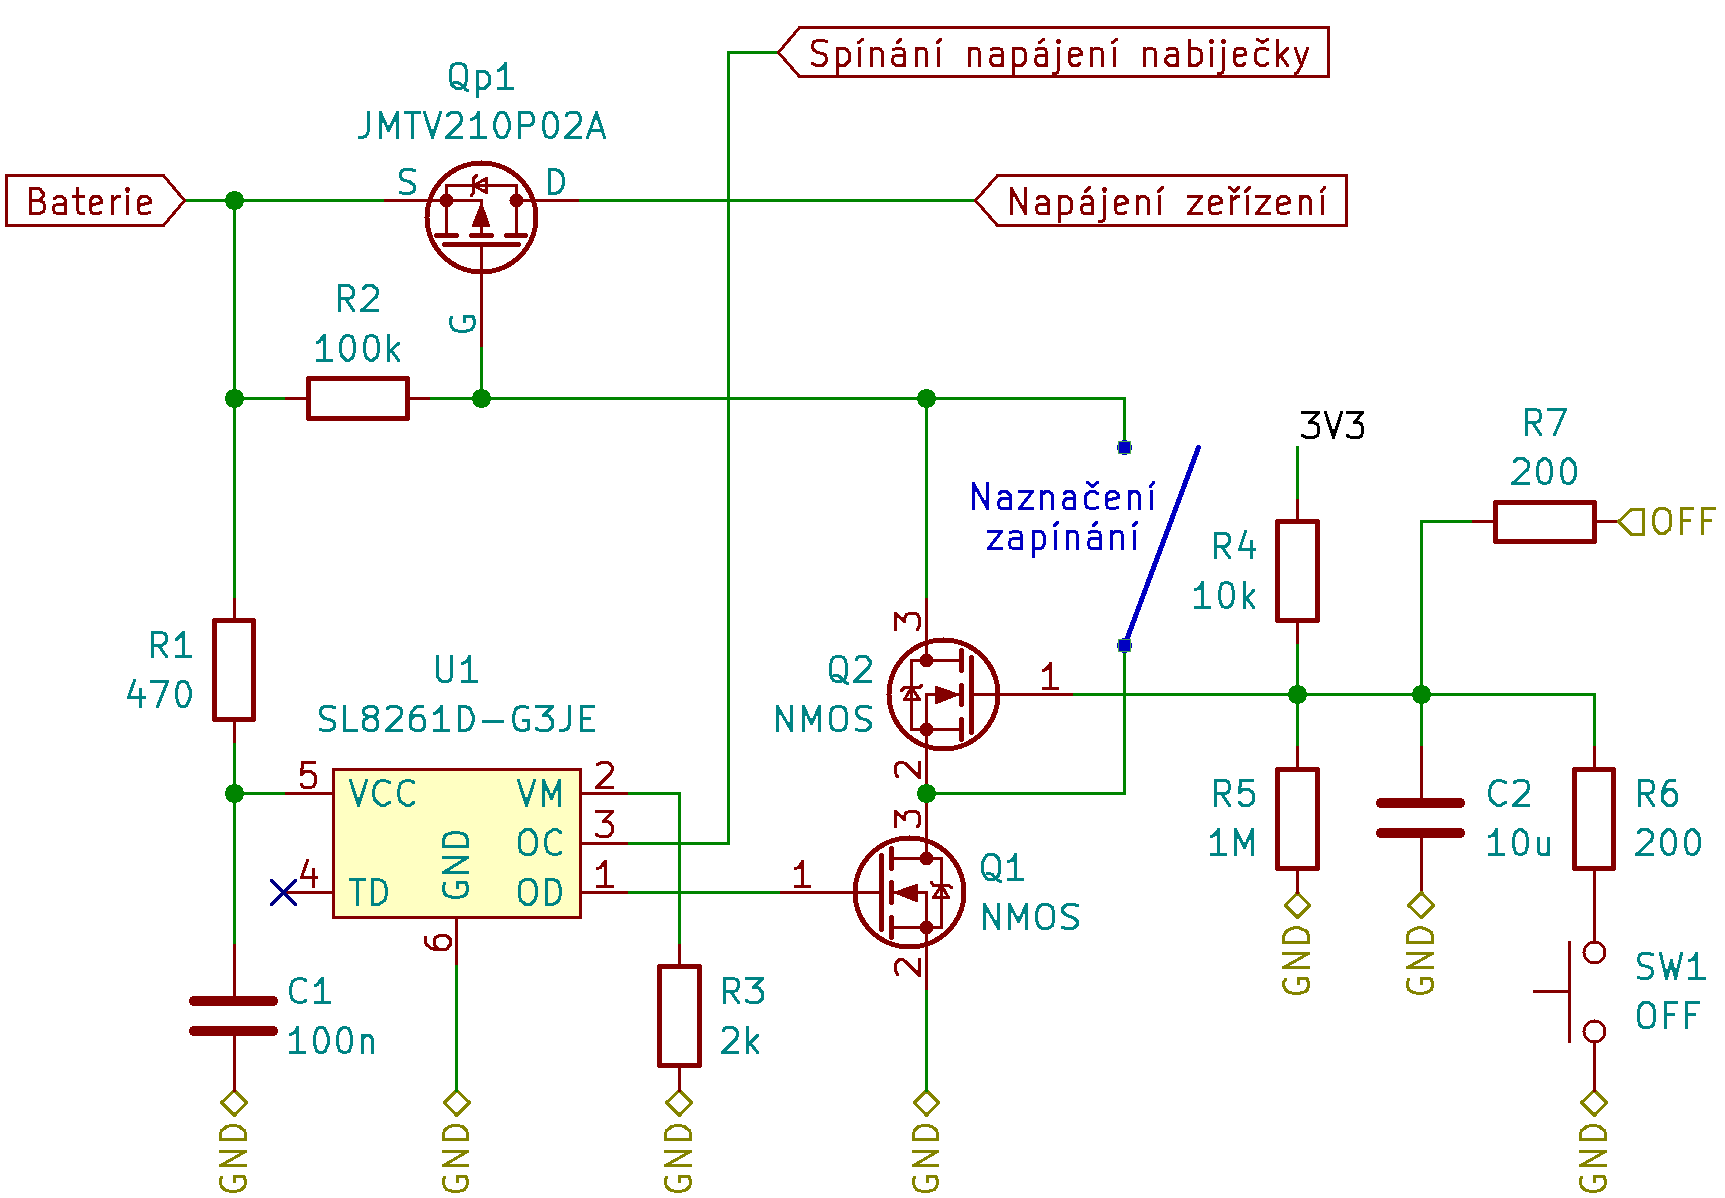
\includegraphics[width=\textwidth]{text/PraktickaCast/img/stary_power_manager.png}
    \caption{Původní verze správy zapínání}
    \label{fig:stary_PoverManager}
\end{figure}

Tato varianta však měla jeden problém způsobený absencí hystereze u~čipu kontrolující napětí baterie SL8261 \cite{SL8261}.
Ve chvíli, kdy se~baterie dostane do~stavu, kdy je~potřeba ji~odpojit, kontrola ji~skutečně odpojí.
To by~bylo správně, jenže z~baterie v~tu~chvíli pořád teče proud, který způsobuje úbytek jejího napětí.
Při přerušení proudu z~baterie se~tak napětí baterie lehce zvedne a~ochrana podbití tak znovu sepne.
Během této doby se~nestihne vybít kapacita na~napájecí větvi a~zařízení se~tak nestihne plně vypnout.
Obvod tak začne oscilovat a~skončí teprve až~napětí na~baterce klesne natolik, aby odpojení znovu nezvedlo napětí nad rozpoznávací úroveň čipu SL8261.

Tento problém má~dvě potenciální řešení.
Buď vyměnit obvod SL8261 za~jiný s~vhodnou hysterezí nebo upravit zapojení tak, aby v~případě, kdy se~čip SL8261 rozhodne zařízení vypnout, se~zařízení stihlo vypnout.
Následně tak už~nezáleží zda kontrola baterie zapnutí opět povolila, protože zařízení je~vypnuto klasickým způsobem.
Tato možnost navíc umožňuje zařízení uživatelsky znovu zapnout a~pokud by~zároveň výrazně klesla spotřeba, zařízení se~ještě chvíli udrží zapnuté a~uživateli tak může zahlásit vybití.
To může být výhodné, např. v~situacích, kdy se~stanoviště vybije ve~chvíli, kdy nikdo není poblíž a~když následně uživatel přijde, nemusí dlouho přemýšlet, co~se~stalo.

Obvod jsem tedy přepracoval a~doplnil jsem do~něj jeden bit paměti, do~kterého může kontrola baterie nebo mikrokontrolér zapsat a~tím zahájit vypínání.
Zároveň jsem odebral vypínací tlačítko s~tím, že~vypínání se~bude provádět programově za~pomoci běžného tlačítka, aby bylo možné nastavit časové chování tlačítka, např. vypnutí až~po delším stisku. 
Ve chvíli, kdy je~vypínání zahájeno, zařízení se~už nedá znovu zapnout až~do doby, než klesne napětí na~napájecí větvi výrazně pod napětí, při kterém by~mohlo dojít k~samovolnému zapnutí (cca \(1.5~V\)).
Výsledný obvod je~vidět na~obr. \ref{fig:PoverManager}.

Hlavní spínač je~v~tomto zapojení PMOS tranzistor \(Q_{p2}\), který je~řízený okolním zapojením.
Přivedením napětí \(0~V\) na~\(G\) tranzistoru \(Q_{p2}\) dojde k~jeho sepnutí a~následnému startu zařízení.
K~tomu může dojít sepnutím NMOS tranzistorů \(Q_{6}\) a~\(Q_{7}\).
Tranzistor \(Q_{4}\) má~stejnou funkci jako tranzistor \(Q_{1}\) v~předchozím zapojení, tedy když obvod \(U_{2}\) rozezná kriticky vybitou baterii, tranzistor rozepne.
Naopak když obvod rozezná nabitou baterii, povolí zapnutí sepnutím tranzistoru \(Q_{4}\).
Ve chvíli, kdy je~zapnutí povoleno a~uživatel stiskne \(ON\)~tlačítko, otevře tranzistor \(Q_{5}\), čímž přivede \(0~V\) na~\(G\) tranzistoru \(Q_{p2}\).
Tranzistor \(Q_{p2}\) se~tak sepne, v~reakci na~což se~uvede do~provozu napájecí větev {\it 3V3}.
To znamená, že~se~začnou skrz rezistory \(R_{12}\) a~\(R_{13}\) nabíjet kapacity \(G\) tranzistorů \(Q_{7}\), \(Q_{8}\) a~\(Q_{6}\).

Tranzistory \(Q_{7}\) a~\(Q_{8}\) spolu s~rezistory \(R_{12}\) a~\(R_{13}\) vytváří dvě do~kruhu zapojené inverze, které tak vytváří jednoduchou paměť.
Stav této paměti je~čitelný na~vývodech \(G\) obou tranzistorů, kde vždy existuje logická nula i~jednička, které se~mohou mezi sebou prohazovat a~tím udržovat informaci.
Zapnutý stav znamená logickou jedničku na~\(G\) tranzistoru \(Q_{7}\) a~nulu na~\(G\) tranzistoru \(Q_{8}\).
Při startu je~nutné, aby toto pořadí naběhlo správně a~nikoliv opačně (což by~znamenalo, že~ihned po~zapnutí dojde k~vypnutí).
Aby tedy se paměť při startu správně inicializovala, mají rezistory \(R_{12}\) a~\(R_{13}\) různé hodnoty, přesněji \(R_{12}\) má~větší odpor a~napětí na~\(G\) tranzistoru \(Q_{8}\) tak bude nabíhat pomaleji.
Napětí na~\(G\) tranzistoru \(Q_{7}\) tak dosáhne jeho otevření dříve, čímž přivede \(0~V\) na~\(G\) tranzistoru \(Q_{8}\), který tak zavře, čímž se~stav paměti ustálí.
Zvláštní hodnota rezistoru \(R_{12}\) je~způsobena snahou o~minimalizaci součástek.
Tuto hodnotu jsem již použil jinde na~zařízení a~abych tedy nemusel přidávat další hodnotu rezistoru, použil jsem tuto.

Aby měly takto vytvořené paměti smysl, je~nutné zajistit, aby žádný ze~zdrojů neměl dvojčinný [push-pull] výstup nebo aby alespoň uměl pracovat v~režimu s~vysokou impedancí.
Výstup z~mikrokontroléru toto umí zajistit jednoduše programově.
Obvod \(U_{1}\) hlídající napětí baterie má~ale výstup dvojčinný z~důvodu potřeby přímého řízení tranzistoru NMOS a~musím ho~to tedy ošetřit jinak.
Zvolil jsem řízení na~straně logické jedničky v~zapnutém stavu, aby vypnutí znamenalo stažení dráhy k~zemi.
Alternativou by~totiž bylo tahat dráhu k~napájecí větvi {\it 3V3}, což by~znamenalo dodatečné zapojení, protože obvod \(U_{2}\) je~napájený jiným napětím než mikrokontrolér a~tedy než tato paměťová buňka.
Mikrokontrolér stažením dráhy \(OFF\) spojí dráhu ze~zemí přes, pro naši úvahu zanedbatelný, ochranný rezistor \(R_{76}\).
Ochrana podbití je~pak připojena přes tranzistor \(Q_{3}\), z~něhož je~využita jen jeho dioda.
Namísto tranzistoru \(Q_{3}\) by~mohla být zapojena jen samostatná dioda, tranzistor je~zde použit z~obdobného důvodu jako zvláštní hodnota rezistoru \(R_{12}\) a~to, aby nebylo nutné do~zařízení přidávat další typ součástky.

Ve chvíli, kdy do~zapojení přijde povel k~vypnutí, zapíše se~povel nejprve do~této paměti.
Toto je~ostatně další důvod, proč se~do paměti zapisuje přes \(G\) tranzistoru \(Q_{7}\) a~ne~\(G\) tranzistoru \(Q_{8}\).
Kdyby totiž zápis probíhal z~druhé strany, zařízení by~se~začalo vypínat už~v~době zápisu do~paměti, protože by~probíhal na~straně, která řídí tranzistor \(Q_{p2}\).
Když tedy dojde k~zápisu do~paměti a~tranzistor \(Q_{p2}\) se~rozepne, začne padat napětí na~napájecí větvi {\it 3V3}, na~rozdíl od~dřívějšího zapojení, ale během toho nemůže dojít k~samovolnému zapnutí.
Protože aby mohlo dojít k~zapnutí, musel by~se~sepnout tranzistor \(Q_{7}\), což se~ale stát nemůže, protože je~sepnut tranzistor \(Q_{8}\). 
Tranzistor \(Q_{8}\) se~rozepne teprve ve~chvíli, kdy napětí na~napájecí větvi {\it 3V3} poklesne natolik, aby už~neudrželo tranzistor sepnutý a~v~tu~chvíli už~nemůže dojít k~sepnutí tranzistoru \(Q_{7}\).

\begin{figure}[h!]
    \centering
    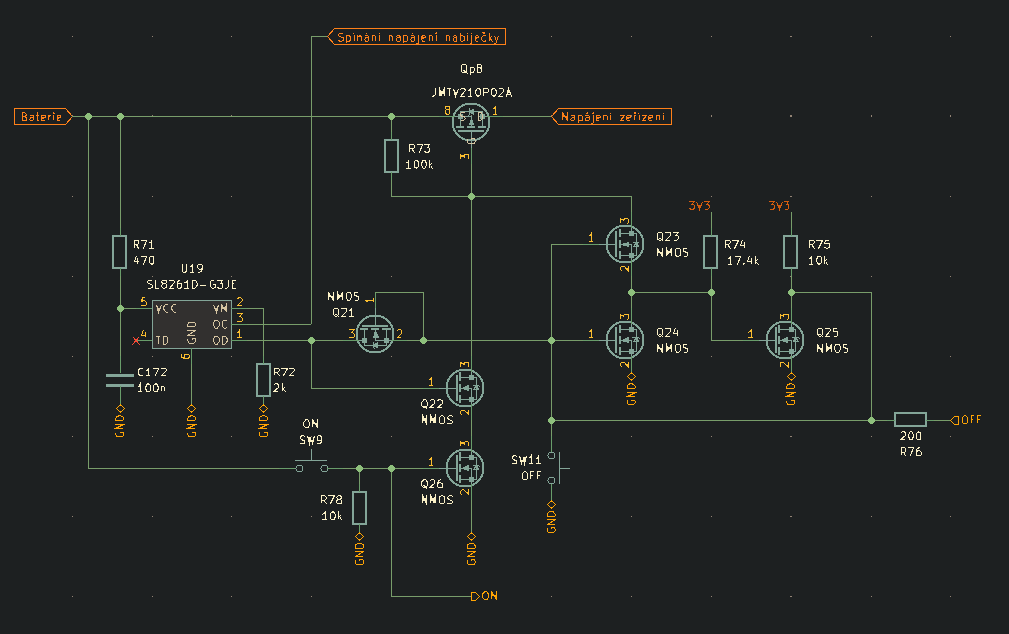
\includegraphics[width=\textwidth]{text/PraktickaCast/img/power_manager.png}
    \caption{Nová verze správy zapínání}
    \label{fig:PoverManager}
\end{figure}

Přestože~\(G\) tranzistoru \(Q_{p2}\) je~řízený stranou paměti \(G\) tranzistoru \(Q_{8}\), tyto dráhy musí být částečně odděleny.
V~případě přímého spojení by~totiž paměťová buňka nemohla správně plnit svoji funkci, protože by~na~ni~bylo skrz rezistor \(R_{11}\) ve~vypnutém stavu přivedeno napětí baterie.
To by~mělo za~následek růst spotřeby ve~vypnutém stavu zaviněný částečným startem zařízení a~především nemožnost normálního startu.
Skrze resistory \(R_{11}\) a~\(R_{12}\) by~se~totiž dostalo napětí baterie na~napájecí větev {\it 3V3}, kde by~mohlo některé systémy uvést do~provozu.
Proud tekoucí přes rezistory \(R_{11}\) a~\(R_{12}\) by~dosahoval řádově desítek mikroampér, což by~spotřebu ve~vypnutém stavu navýšilo přibližně o~řád.
Významnější problém by~ale byl otevřený tranzistor \(Q_{8}\), který by~tak držel zavřený tranzistor \(Q_{7}\), což by~znemožnilo nemožnost správného startu zařízení.
Řešením tohoto problému je~tranzistor \(Q_{6}\), který se~sepne jen ve~chvíli, kdy je~v~paměti zapsána správná hodnota.
Tehdy je~jeho \(S\) připojeno skrze tranzistor \(Q_{7}\) k~zemi a~jeho \(G\) skrze rezistor \(R_{13}\) k~napětí \(3,3~V\) a~je~tedy plně otevřen.
Naopak ve~chvíli, kdy je~do paměti zapsán povel k~vypnutí, je~na jeho \(S\) připojeno skrze rezistor \(R_{12}\) napětí napájecí větve {\it 3V3} a~jeho \(G\) skrze tranzistor \(Q_{8}\) k~zemi a~je~tedy plně uzavřen.
Tímto způsobem je~tedy zajištěno oddělení paměťové buňky od~\(G\) tranzistoru \(Q_{p2}\).

\subsection{Výkonová napájecí větev}
Jako napájecí napětí pro výkonové části zařízení slouží napětí \(5~V\), protože toto napětí využívají světelné kruhy, skládající se~z~LED WS2812 \cite{WS2812B}.
Tyto LED mají rozsah napájecího napětí \(3,5\) až~\(5,3~V\), a~právě proto volím napájecí napětí \(5~V\).
Stačilo by~sice i~napětí nižší, ale s~větví \(3,3~V\) bych výkonovou větev tak jako tak nespojil.
Především by tak však byl nutný složitější spínaný zdroj, který by~musel spínat nejen na~vyšší napětí, ale i~na~nižší, podle toho jaké napětí je~zrovna na~baterii.
Navíc je~napětí \(5~V\) vhodný i~pro napájení na~modulovém konektoru.

Vznikají tak dva systémy, které jsou napájeny napětím \(5~V\), především LED kruhy ale také moduly připojené na~modulovém konektoru.
Protože oba tyto systémy mohou mít nezanedbatelnou spotřebu i~ve~chvíli, kdy nejsou používány, je~vhodné mít možnost odpojit je~od napájení.
Použité LED mají totiž spotřebu i~ve vypnutém stavu \(0,5~mA\), což při počtu \(120\) LED dělá klidovou spotřebu \(60~mA\).
U~modulu toto sice neumím říct dopředu, ale dá se předpokládat, že bude výhodné moduly vypínat.

Čím jemnější dělení, tím lépe půjde optimalizovat spotřeba.
Protože jsou všechny moduly připojeny na~stejném konektoru, znamená to~dvě samostatně řiditelné větve.
Navíc je~vhodné vypínat i~samotný zdroj obou větví ve~chvíli, kdy není využíván.
Za tímto účelem jsem tedy implementoval schéma na~obr.\ref{fig:spinac_vikonove_vetve}

\begin{figure}[h!]
    \centering
    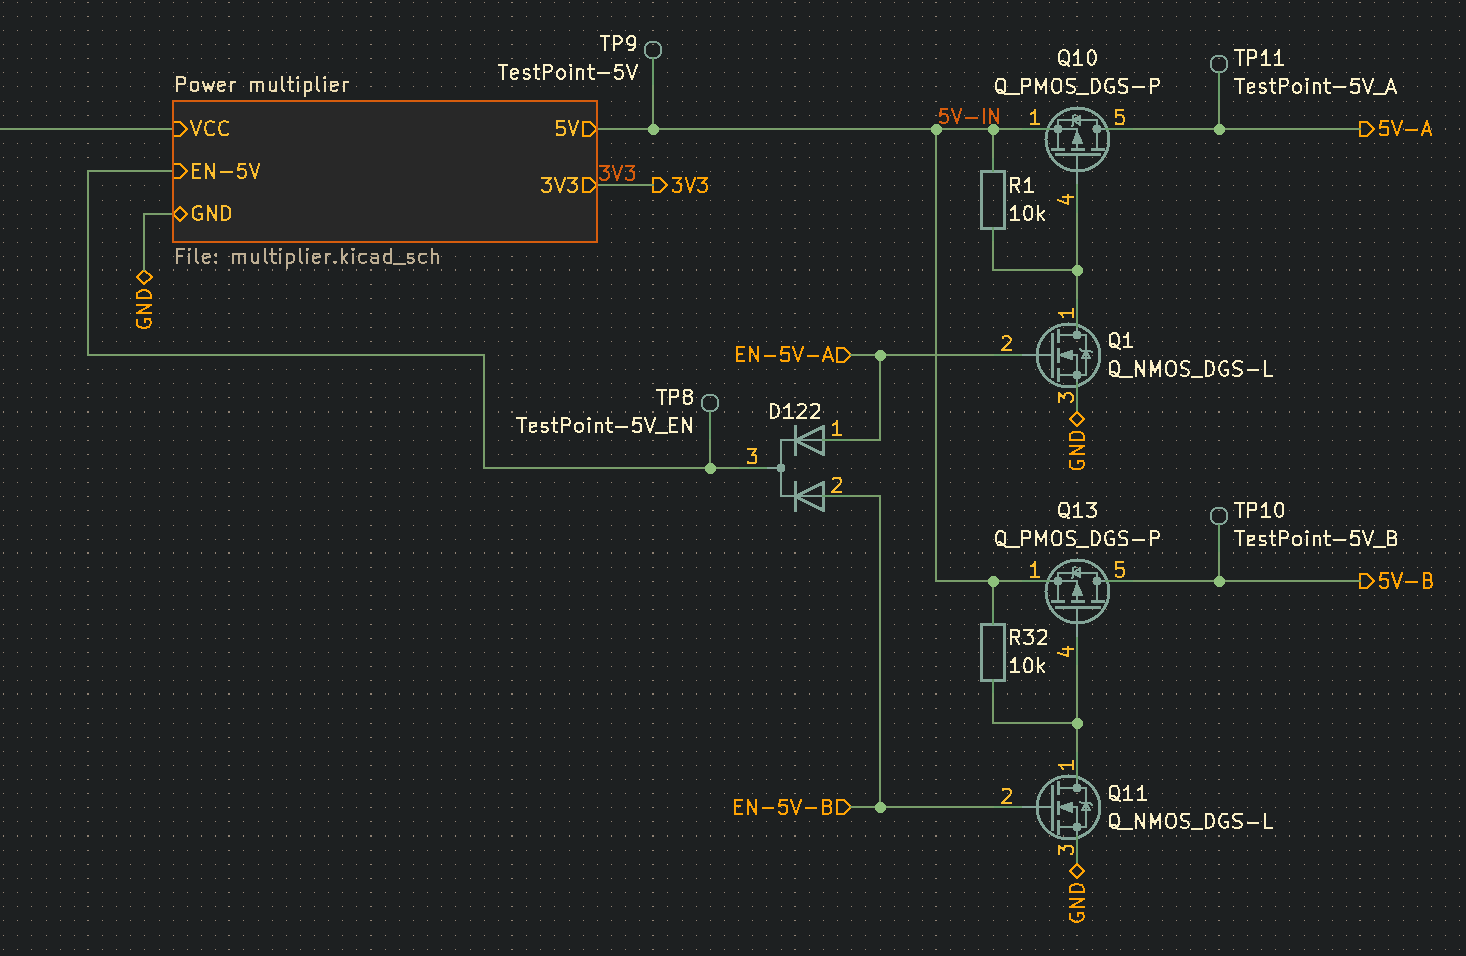
\includegraphics[width=\textwidth]{text/PraktickaCast/img/spinac_vikonove_vetve.png}
    \caption{Spínač výkonové větve}
    \label{fig:spinac_vikonove_vetve}
\end{figure}

Výchozí stav vstupů {\itshape EN-5V-A} a~{\itshape  EN-5V-B} je~\(0~V\), což je~definováno pomocí rezistorů, které tyto dráhy připojuje k~zemi.
Tyto rezistory však ve~schématu na~obr.\ref{fig:spinac_vikonove_vetve} nenajdete, protože jsou součástí schématu s~mikrokontrolérem.
Tam jsou zároveň použity k~definici výchozího stavu pinů {\it IO45} a~{\it IO46}, které se~používají při startu procesoru.
Ve výchozím stavu drah {\itshape EN-5V-A} a~{\itshape EN-5V-B} je~tedy \(0~V\), což znamená rozpojené tranzistory \(Q_9\) a~\(Q_{10}\).
Výsledkem rozpojení tranzistorů \(Q_9\) a~\(Q_{10}\) je~tedy za~pomocí rezistorů \(R_{15}\) a~\(R_{32}\) i~rozpojení tranzistorů \(U_{9}\) a~\(U_{15}\).
Současně s~tím je~\(0V\) i~na~dráze {\itshape EN-5V}, která řídí spínaný zdroj základní pěti voltové větve.
Výchozí stav této dráhy je~opět definovaný připojením k~zemi přes rezistor, který je~tentokrát umístěn ve~schématu spínaného zdroje.
Ve chvíli, kdy dojde z~procesoru povel k~zapnutí jedné z~větví, řekněme větve {\itshape 5V-A}, mikrokontrolér přivede napětí \(3,3~V\) na~dráhu {\itshape EN-5V-A}.
Tedy přivede napětí \(3,3~V\) na~\(G\) tranzistor \(Q_9\), čímž jej sepne a~zároveň skrze jednu diodu \(D_{122}\) na~{\itshape EN-5V}, čímž uvede do~provozu spínaný zdroj a~tedy přivede napětí na~dráhu \(5V\).
Následkem sepnutí tranzistoru \(Q_9\) se~přivede \(0~V\) na~\(G\) tranzistoru \(U_{9}\), čímž se~sepne a~přivede napětí \(5V\) na~dráhu {\itshape 5V-A}.
Obdobně pak v~případě aktivace dráhy {\itshape 5V-B}.

%~\newpage

\subsection{Jednoduchá signalizační LED}

Pro signalizaci některých stavů jsem do~zařízení přidal i~obyčejnou RGB LED.
Je~řiditelná z~mikrokontroléru, ale ve~chvíli, kdy ji~mikrokontrolér aktivně neřídí, může slabým svitem signalizovat i~některé hardwarové stavy.
Červeným kanálem signalizuje, že~je zařízení v~chodu a~modrým kanálem informuje o~stavu nabíjení.
Když nabíjení probíhá, svítí modrý kanál trvale.
Když nabíjení neprobíhá, např. když je~dokončeno, modrý kanál nesvítí a~v~případě, že~nabíjecí obvod BQ25895 \cite{BQ25895} detekuje nějaký problém, bliká s~frekvencí \(1 Hz\).
Zapojení LED je~vidět na obr. \ref{fig:hloupa-LED}.

\vspace{-3mm}
\begin{figure}[h!]
    \centering
    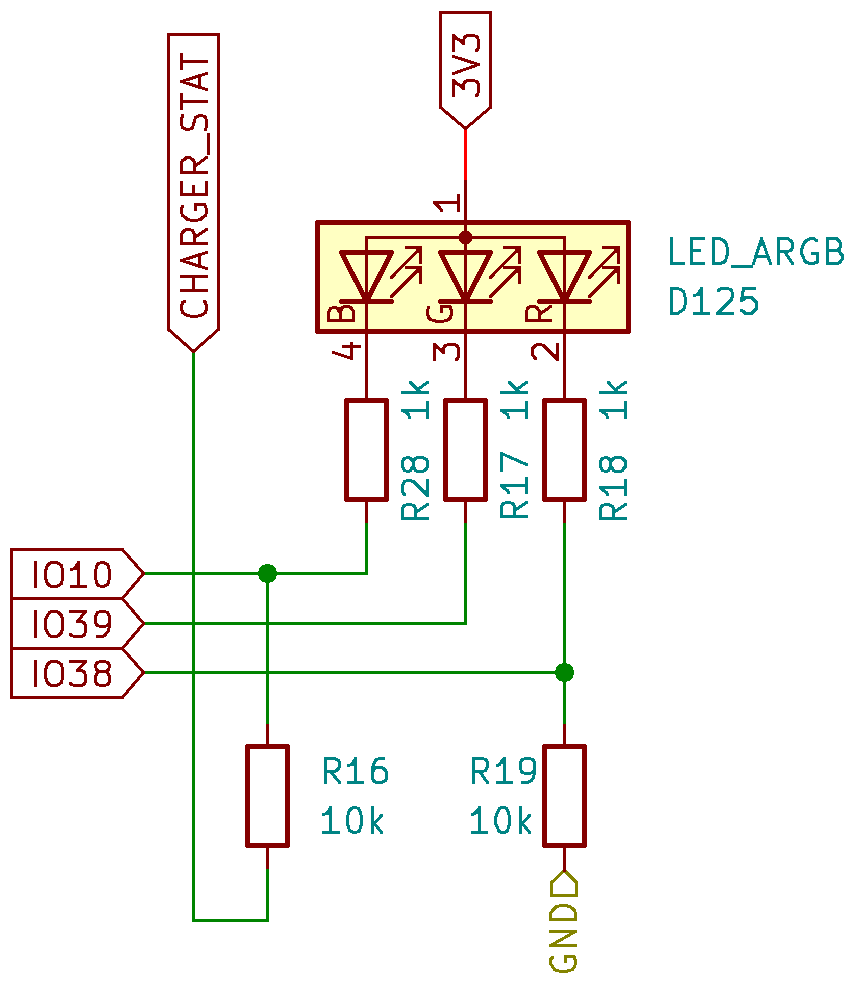
\includegraphics[angle=-90,width=0.585\textwidth]{text/PraktickaCast/img/RGB-LED.png}
    \caption{Zapojení prosté signalizační RGB LED}
    \label{fig:hloupa-LED}
\end{figure}
\vspace{-2mm}

Zdvojení řízení LED umožňují dodatečné odpory \(R_{16}\) a~\(R_{19}\).
Ve chvíli, kdy je~tak např. pin mikrokontroléru pin \(IO38\) ve~stavu vysoké impedance, je~červený kanál diody vlastně připojen přes odpor \(11~k\Omega\) k~zemi.
Výsledný jas diody sice není vysoký, ale informaci uživateli předá.

\subsection{Odhad spotřeby zařízení}
Spotřeba zařízení bude silně záviset na~typu využívání.
Některé hry například mohou vyžadovat jen jednu-dvě svítící LED naráz a~jiné naopak mohou pracovat se~všemi naráz.
Navíc budou spotřebu ovlivňovat aktuálně připojené moduly.
Pro odhad tedy budu předpokládat spíše náročnější podmínky, aby byl odhad spíše skeptický.

Předpokládám využití jednoho světelného kruhu s~osmdesáti procentním jasem jednoho kanálu LED.
Zároveň předpokládám běžící tlakovou plochu a~bezdrátovou komunikaci.
U spínaného zdroje, který zprostředkovává napájení větve \(U_{OUT} = 5~V\) předpokládám efektivitu \(\mu = 95\-\%\) \cite{TPS61088}.
Nakonec aktuální napětí baterie \(U_{bat} = 3,5~V\). 

\begin{itemize}
    \item LED WS2812 \cite{WS2812B-cinsky}
    \begin{itemize}
        \item spotřeba jednoho kanálu je~dle dokumentace \(12~mA\), při osmdesáti procentním jasu tedy \(I_{LED-k} = 9,6~mA\)
        \item fixní spotřeba řídící elektroniky celé LED \(I_{LED-d} = 0,5~mA\)
    \end{itemize}
    \item Moduly 
    \begin{itemize}
        \item průměrnou spotřebu modulu předpokládám na~\(I_{mod} = 50~mA\) (předpokládám, že moduly budou pracovat jen malé procento času) 
    \end{itemize}
    \item Tlaková plocha
    \begin{itemize}
        \item spotřeba LDC1614 je~\(I_{LDC} = 35~\mu A\) \cite{LDC1614}
    \end{itemize}
    \item ESP32-S3
    \begin{itemize}
        \item spotřebu při využívání WiFi odhaduji na~základě měření uvedeného v~dotazu na ESP32 foru \cite{spotreba-ESP32S3} jako \(I_{ESP} = 150~mA\)
    \end{itemize}
\end{itemize}

\vspace{5mm}
\large
\begin{centering}
\(
    I_{bat} = \frac{U_{OUT}}{U_{bat} \cdot \mu} \cdot (60 \cdot (I_{LED-k} + I_{LED-d}) + I_{mod}) + I_{LDC} + I_{ESP} = 
    \frac{5}{3.5 \cdot 0.95} \cdot (60 \cdot (12\cdot10^{-3} \cdot 0.8 + 0.5\cdot10^{-3}) + 50\cdot10^{-3}) + 35\cdot10^{-3} + 150\cdot10^{-3} = 1.17~[A]
\)
\end{centering}
\normalsize
\vspace{1mm}

Při kapacitě jednoho článku baterie \(C_{čla} = 3400~mAh\) \cite{kapacita-18650}, tedy dvojnásobné kapacitě celé baterie, tak můžeme určit výdrž na~jedno nabití jako:

\vspace{3mm}
\large
\( t_{vyd} = \frac{2 \cdot C_{čla}}{I_{bat}} = \frac{2 \cdot 3.4}{1.17} = 5.8 [h] \)  \normalsize resp. \( 5~hodin + 48~minut \)
\vspace{3mm}

To sice vychází na~trochu míň, než jsem na~začátku kapitoly požadoval, ale dá se~předpokládat, že během nastavování bude spotřeba nižší.
Předpokládám totiž, že při nastavování nebudou LED svítit tak vysokým jasem.
% Dost možná nebudou svítit vůbec, protože se~vše nastaví z~telefonu.


Kromě spotřeby za provozu je~také vhodné určit spotřebu zařízení ve~vypnutém stavu.
Nebylo by totiž vhodné, aby během nečinnosti došlo k~podbití baterie a~tím pádem k~jejímu poškození.

Na spotřebu ve~vypnutém stavu má vliv několik součástek.
Jde především o~proud, tekoucí do~nabíjecího obvodu bq25895M \cite{BQ25895}, ale také o~ochranu baterie SL8261D \cite{SL8261} a~několik tranzistorů v~zapínacím obvodu uvedeném na~obr.~\ref{fig:PoverManager}.

\begin{itemize}
    \item Dokumentace nabíjecího obvodu bq25895M \cite{BQ25895} udává spotřebu ve~stavu nečinnosti \(I_{nab} = 12~\mu A\).
    \item Ochrana baterie SL8261D \cite{SL8261} udává spotřebu v~sepnutém stavu \(I_{och} = 3~\mu A\).
    \item Hlavní spínací MOS transistor \cite{WSD20L75DN33} udává proud v~rozepnutém stavu maximálně \(I_{PMOS} = 1~\mu A\).
    \item Dva logické MOS transistor \cite{N-MOS} udává proud v~rozepnutém stavu maximálně \(I_{NMOS} = 1~\mu A\).
\end{itemize}

Výslednou spotřebu ve~vypnutém stavu tak můžeme určit jako:

\vspace{5mm}
\large
\begin{centering}
\(
    I_{vyp} = I_{nab} + I_{och} + I_{PMOS} + I_{NMOS} = (12 + 3 + 1 + 1) \cdot 10^{-6} = 17 [\mu A]
\)
\end{centering}
\normalsize
\vspace{1mm}

Při této spotřebě tedy určíme dobu za kterou by se~zařízení vybilo jako:

\vspace{5mm}
\large
\begin{centering}
\(
    t_{vyd} = \frac{2 \cdot C_{čla}}{I_{vyp}} = \frac{2 \cdot 3.4}{17 \cdot 10^{-6}} = 3.9\cdot10^{5}~[h] \) resp. \(\frac{3.9\cdot10^{5}}{24\cdot365} \approx 46~[let]\)
\end{centering}
\normalsize
\vspace{1mm}

Spotřeba ve~vypnutém stavu je~tedy víc než dostatečně malá.
Nepodařilo se~mi najít hodnoty samovybíjení použitých článků, ale dá se~předpokládat, že budou řádově větší než spotřeba elektroniky ve~vypnutém stavu.

\section{Mechanická stavba}
Celé zařízení bude mít tvar krátkého válce.
Na~horní stranu je~umístěn axiální světelný kruh, do~kterého je~umístěna tlaková plocha.
Na bocích je~pak umístěn radiální světelný kruh a~základní uživatelské ovládání.

Z~důvodu minimalizace součástí je~výhodné LED radiálního světelného kruhu umístit na~LED desku místo na~samostatný díl.
Zároveň je~to způsob, jak se~vyhnout montáži současně radiální i~axiální.
Na prvním prototypu jsem totiž zvolil možnost osadit jen axiální kruh a~radiální jsem vytvořil pomocí LED pásku, který jsem omotal kolem krytu zařízení.
Výsledkem byla neprakticky komplikovaná montáž, kterou se~i~touhle cestou snažím co~možná nejvíc zjednodušit bez ztráty výsledné kvality.

Axiální kruh osazený přímo na~DPS ovšem znamená další komplikaci, jeho účelem je~totiž svítit ve~směru rovnoběžném s~plochou DPS.
Použité LED tedy musí svítit v~ose~rovnoběžné s~plochou desky.
To se~dá zařídit buď do~strany svítícími LED nebo zajistit odraz světla do~stran, tak aby mohly diody svítit ve~směru kolmém na~plochu DPS a~aby přesto vzniklý světelný kruh svítil radiálně.

Do strany svítící inteligentní LED sice existují, ale nemají vhodné rozměry a~navíc jsou výrazně dražší.
Proto jsem se~rozhodl použít stejné diody jako na~axiálním kruhu a~doplnit tělo zařízení o~odraznou plochu, která zajistí správný výsledný směr světla.
Zároveň, abych pokud možno zachoval rozlišitelnost jednotlivých LED, jsem mezi ně~přidal přepážky.
Jejich cílem je~minimalizovat přesvity jednotlivých diod do~prostor diod sousedních.
Obojí je~vidět na~obr.\ref{fig:AHS-radializatoru}.

\begin{figure}[h!]
    \begin{minipage}{0.5\textwidth}
        \centering
        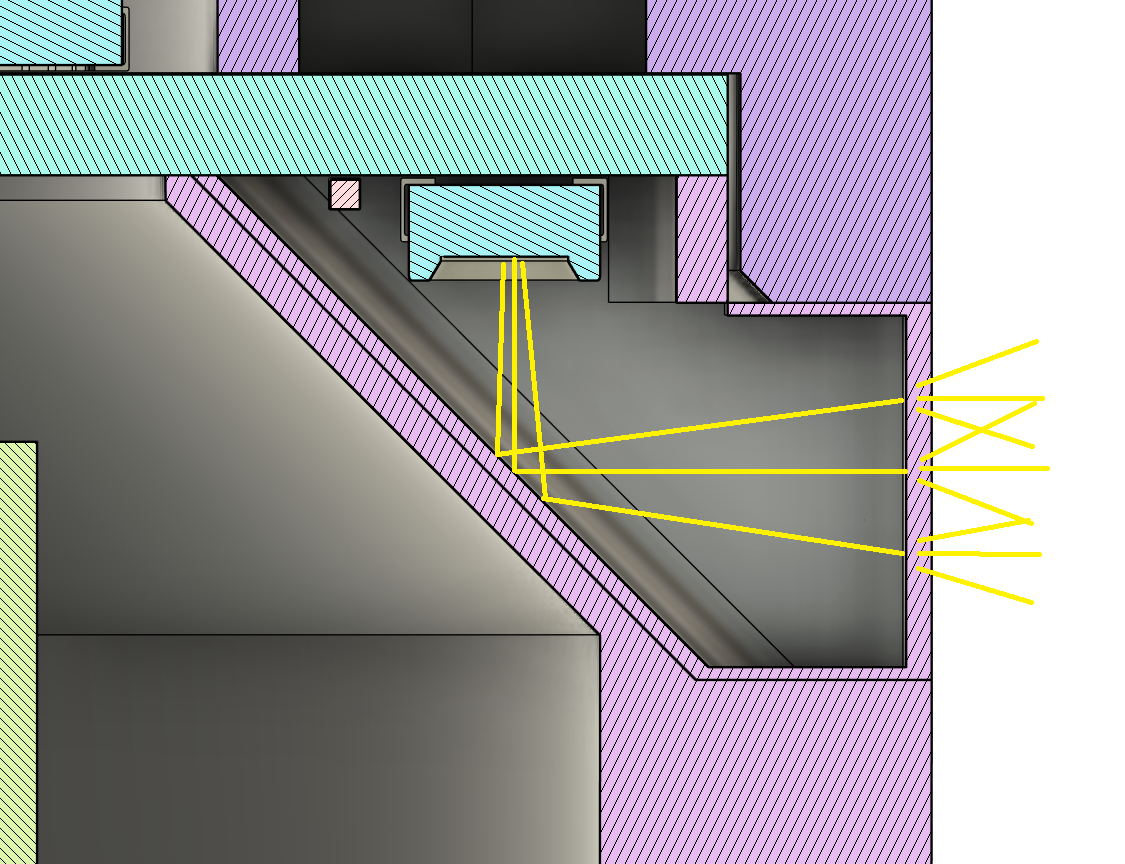
\includegraphics[width=\textwidth]{text/PraktickaCast/img/AHS-odrazkaRozptylka.png}
    \end{minipage}
    \begin{minipage}{0.5\textwidth}
        \centering
        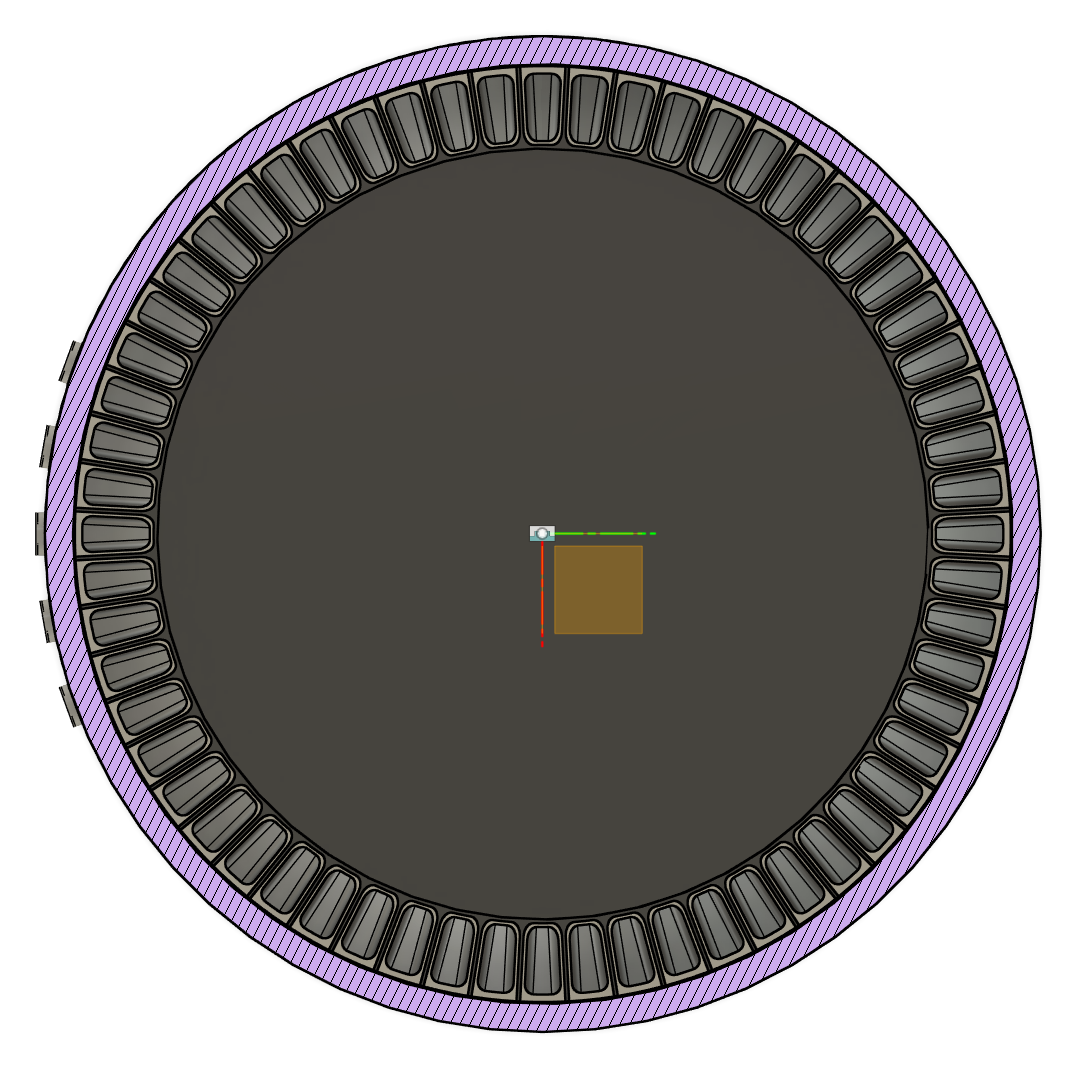
\includegraphics[width=\textwidth]{text/PraktickaCast/img/AHS-prepazky.png}
    \end{minipage}
    \caption{Odrazná plocha a~přepážky Radiálního světelného kruhu}
    \label{fig:AHS-radializatoru}
\end{figure}

Významnou mechanickou částí je~také uložení tlakové plochy.
Tento systém se~skládá ze~snímací části, která je~součástí LED desky a~snímané části, terčíků, se~kterou je~v~kontaktu uživatel.
Terčíky se~musí při používání pohybovat, sice málo ale za~to konzistentně, aby bylo možné výsledek použít jako ovládací prvek.
Protože se~navíc tlaková plocha nachází uvnitř axiálního světelného kruhu, je~nutné, aby byl terčík buď průsvitný nebo uchycený až~uvnitř kruhu.
Uchycení uvnitř kruhu by~ale znamenalo zmenšení snímatelné plochy a~potřebu poměrově výraznějších deformací, aby se~dosáhlo stejné změny indukčnosti.
Abych minimalizoval velikost nesnímaných okrajů, rozhodl jsem se~pro průsvitnou variantu.

V~první verzi jsem tedy terčíky řešil tenkým plošným spojem, na~kterém jsem odleptal vše kromě kruhu o~něco málo menšího než vnitřní průměr světelného kruhu.
Měď tak sloužila jako vodivý terčík.
Sklolaminát, který tvoří nosnou část DPS, sice není úplně čirý a~způsobuje tak difuzi světla, ta~ale v~tomto případě nevadí.
Tuto DPS jsem následně přilepil na~tělo zařízení, těsně nad LED desku na~mezikruží obklopující světelný kruh.
Zvolil jsem tedy \(0.6~mm\) tlustá FR4 DPS.
Tloušťku jsem zvolil tak, abych umožnil co~možná největší deformace a~ulehčil tak rozlišování skutečného stisku od~nežádoucího šumu.

Tato metoda však měla pár nedostatků.
Především \(0.6~mm\) tlustá FR4 DPS nebyla dostatečně stálá a~docházelo k~její postupné trvalé deformaci.
Po několika měsících tak DPS začala tvarem připomínat misku, což vedlo k~porušení lepidla a~bylo tak nutné ji~lepit znovu.
Rozhodl jsem se~proto DPS zesílit, aby trvalým deformacím lépe odolala.

%~Rozhodl jsem se~proto vyzkoušet dvě alternativní řešení:
%~\begin{enumerate}
%~    \item Tlustší FR4 DPS
%~    \item DPS s~hliníkovým jádrem
%~\end{enumerate}

%~Tlustší FR4 DPS by~měla výhodu v~tom že~je principiálně stejná jako předchozí varianta a~vyžadovala by~tedy jen minimální upravu.
%~Nevýhodou by~naopak mohl být stále stejný problém s~tím že~by se~jen prodloužil čas kdy funguje dle požadavku. 
%~DPS s~hliníkovým jádrem by~měla naopak výhodu stálosti ale zase~by~se~objevil problém s~průsvitností.

%~Rozhodl jsem se~tedy vyzkoušet obojí

Samotný kryt zařízení jsem rozdělil na~několik částí, jejichž sestava je~vidět na~obr.\ref{fig:AHS-kryt}
\begin{itemize}
    \item Hlavní tělo, jehož součástí je~odrazná plocha pro radiální světelný kruh a~hmatník tlačítek, který je~součástí těla z~důvodu těsnosti zařízení
    \item Horní okraj, který překrývá okraje LED desky a~usazuje DPS terčíku
    \item Zadní víko, které se~šroubuje do~závitu v~hlavním těle a~zajišťuje tak uchycení hlavní desky a~zároveň uzavírá zařízení
    \item Distanční přítlačná vložka, zajištující rovinnost plochy hlavní desky v~místech kontaktu s~šroubovacím víkem
    \item Dodatečný díl, který by~ideálně byl součástí hlavního těla, ale pro usnadnění tisku je~oddělen, tisknut zvlášť a~následně pomocí pozičních výstupků zapozicován a~nalepen k~hlavnímu tělu  ~
\end{itemize}

\begin{figure}[h!]
    \centering
    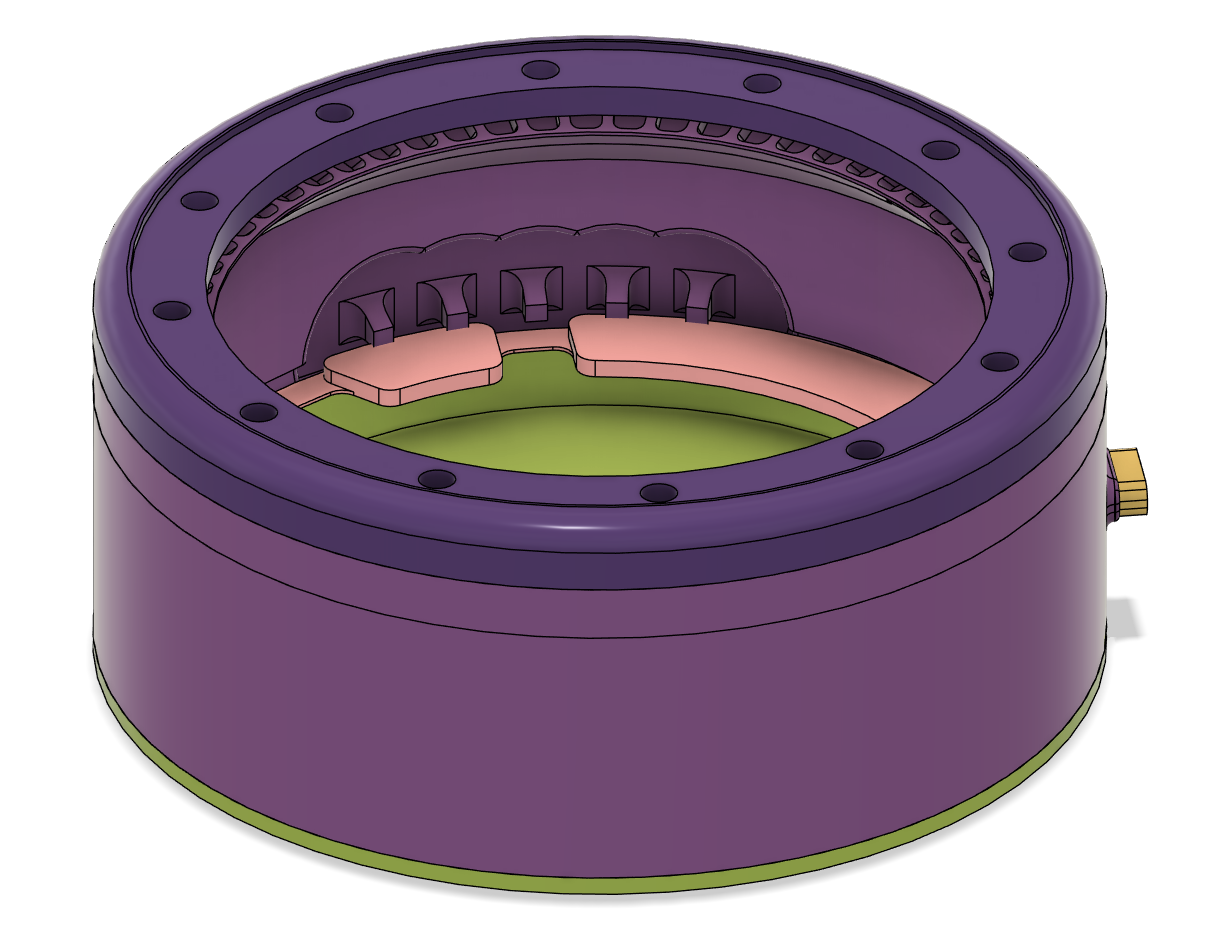
\includegraphics[width=\textwidth]{text/PraktickaCast/img/Kryt-Lucerny.png}
    \caption{Sestava krytu bez elektroniky a~terčíku tlakové plochy}
    \label{fig:AHS-kryt}
\end{figure}

\chapter{Návrh dynamického zařízení}
% Uživatelským požadavkem je dynamické zařízení sloužící například jako identifikátor hráče, nebo jako herní nástroj.
% Mělo by ale být schopno zastat i~roli statického zařízení, pro případy her na delších výletech, kde by bylo nepraktické nosit s~sebou velké zařízení.
% Vyžaduje tedy dostatečnou mobilitu, aby uživateli nepřekáželo v~pohybu.
% Zároveň by zařízení mělo být co nejlevnější pro možnost nasazení ve velkém počtu.
% Z~toho plynou požadavky na výslednou konstrukci a velikost zařízení.

% Zařízení by mělo být schopno komunikovat s~ostatními zařízeními, ať už statickými nebo dynamickými.
% Potřebuje také světelný výstup pro zobrazování herních stavů a~jednoduchý vstup pro ovládání.

% % realizace

Pro přehlednost by zařízení mělo mít jméno a protože může často sloužit podobně jako semafor, začal jsem mu říkat Semisemafor.

Vstup bude realizován pomocí dvou tlačítek a šestiosého IMU, pro možnost používání gest.

Světelný výstup bude realizován pomocí dvanácti RGB LED uspořádaných do kruhu.
Číslo dvanáct bylo zvoleno proto, aby korespondovalo s hodinami, např. pro hry, kde probíhá nějaký odpočet.

Aby nebylo nutné starat se o baterii, bylo napájení zajištěno pomocí USB-A konektoru a~malé powerbanky, která se tak dá třeba i snadno vyměnit za nabitou.

\section{Výběr součástek}
Protože zařízení bude vyráběno u firmy JLCPCB, je výhodné využívat součástky, které mají ve své nabídce.
Dá se sice zařídit, aby firma osadila i součástky od externího dodavatele, ale je to o něco složitější a je tak jednodušší se tomu vyhnout.

Aby nebylo nutné pro práci se semaforem a AHS používat různá prostředí, je výhodné použít stejný kontroler nebo alespoň kontroler ze stejné rodiny.
Proto byl zvolen kontroler ESP32-C3-MINI-1, který je ve srovnání s ESP32-S3 výrazně levnější a aplikaci plně dostačuje. 
ESP32-S3 má stejně jako ESP32-S3 USB periferii, která se dá využít na programování kontroleru.
I~tady je ale problém, že se tato metoda dá softwarově narušit a~Semisemafor je proto vybaven stejným programovacím konektorem jako ESP32-S3 na AHS.

Protože mám dobré zkušenosti s inteligentními ledkami WS2812, zvolil jsem na led kruh jejich typickou pětimilimetrovou variantu.

IMU by na semaforu nemělo sloužit pro žádná přesná měření, ale jen např. pro detekci plácnutí nikoliv jeho síly nebo rychlosti, nezáleží proto tolik na jeho přesnosti.
Při jeho výběru šlo proto primárně o cenu a zvoleno bylo LIS2DH12TR \cite{LIS2DH12TR}, které komunikuje po SPI.

Kontroler ESP32-C3 i LIS2DH12TR má rozsah napájecího napětí do \(3.6 [V]\) \cite{ESP32C3}\cite{LIS2DH12TR}.
Není proto možné je napájet přímo z napětí na USB, na kterém je napětí \(5 [V]\) a bude tedy potřeba měnič.
ESP32-C3 požaduje zdroj se schopností dodat \(0.5 [A]\) \cite{ESP32C3} a jeho typická spotřeba ze zkušenosti nepřesáhne \(200 [mA]\), LIS2DH12TR pak vyžaduje zanedbatelných \(185 [uA]\) (v závislosti na vzorkovací frekvenci i mnohem méně \cite{LIS2DH12TR} strana 17 tabulka 12).
Považuji proto za vhodné pro jeho napájení použít LDO.
Z nabídky JLCPCB byl proto zvolen LD39200 \cite{LD39200} pro jeho elektrické parametry a~malé pouzdro.

\section{Návrh schematu a DPS}

Doplnil jsem blokovací kondenzátory dle doporučení výrobců, pull-up rezistory na~straping pin kontroleru, zpětnovazební dělič k LDO, k~tlačítkům sem připojil kondenzátor proti odskokům.
Dostal jsem tak schéma \ref{Semisemafor-sch-v1}, ze kterého jsem následně nakreslil DPS \ref{Semisemafor-pcb-v1}

\section{Prototypy}

Při testování první verze, byl problém s neovladatelnými ledkami.
Při pokusu o nastavení barvy se jen náhodně rozsvěcovali a zhasínali.
Když jsem připojil osciloskop na jejich řídící signál, obdržel jsem signál \ref{Semisemafor-zvonek} % TODO: změřit znovu a dodat hesží graf

\begin{figure}[!h]
  \begin{center}
    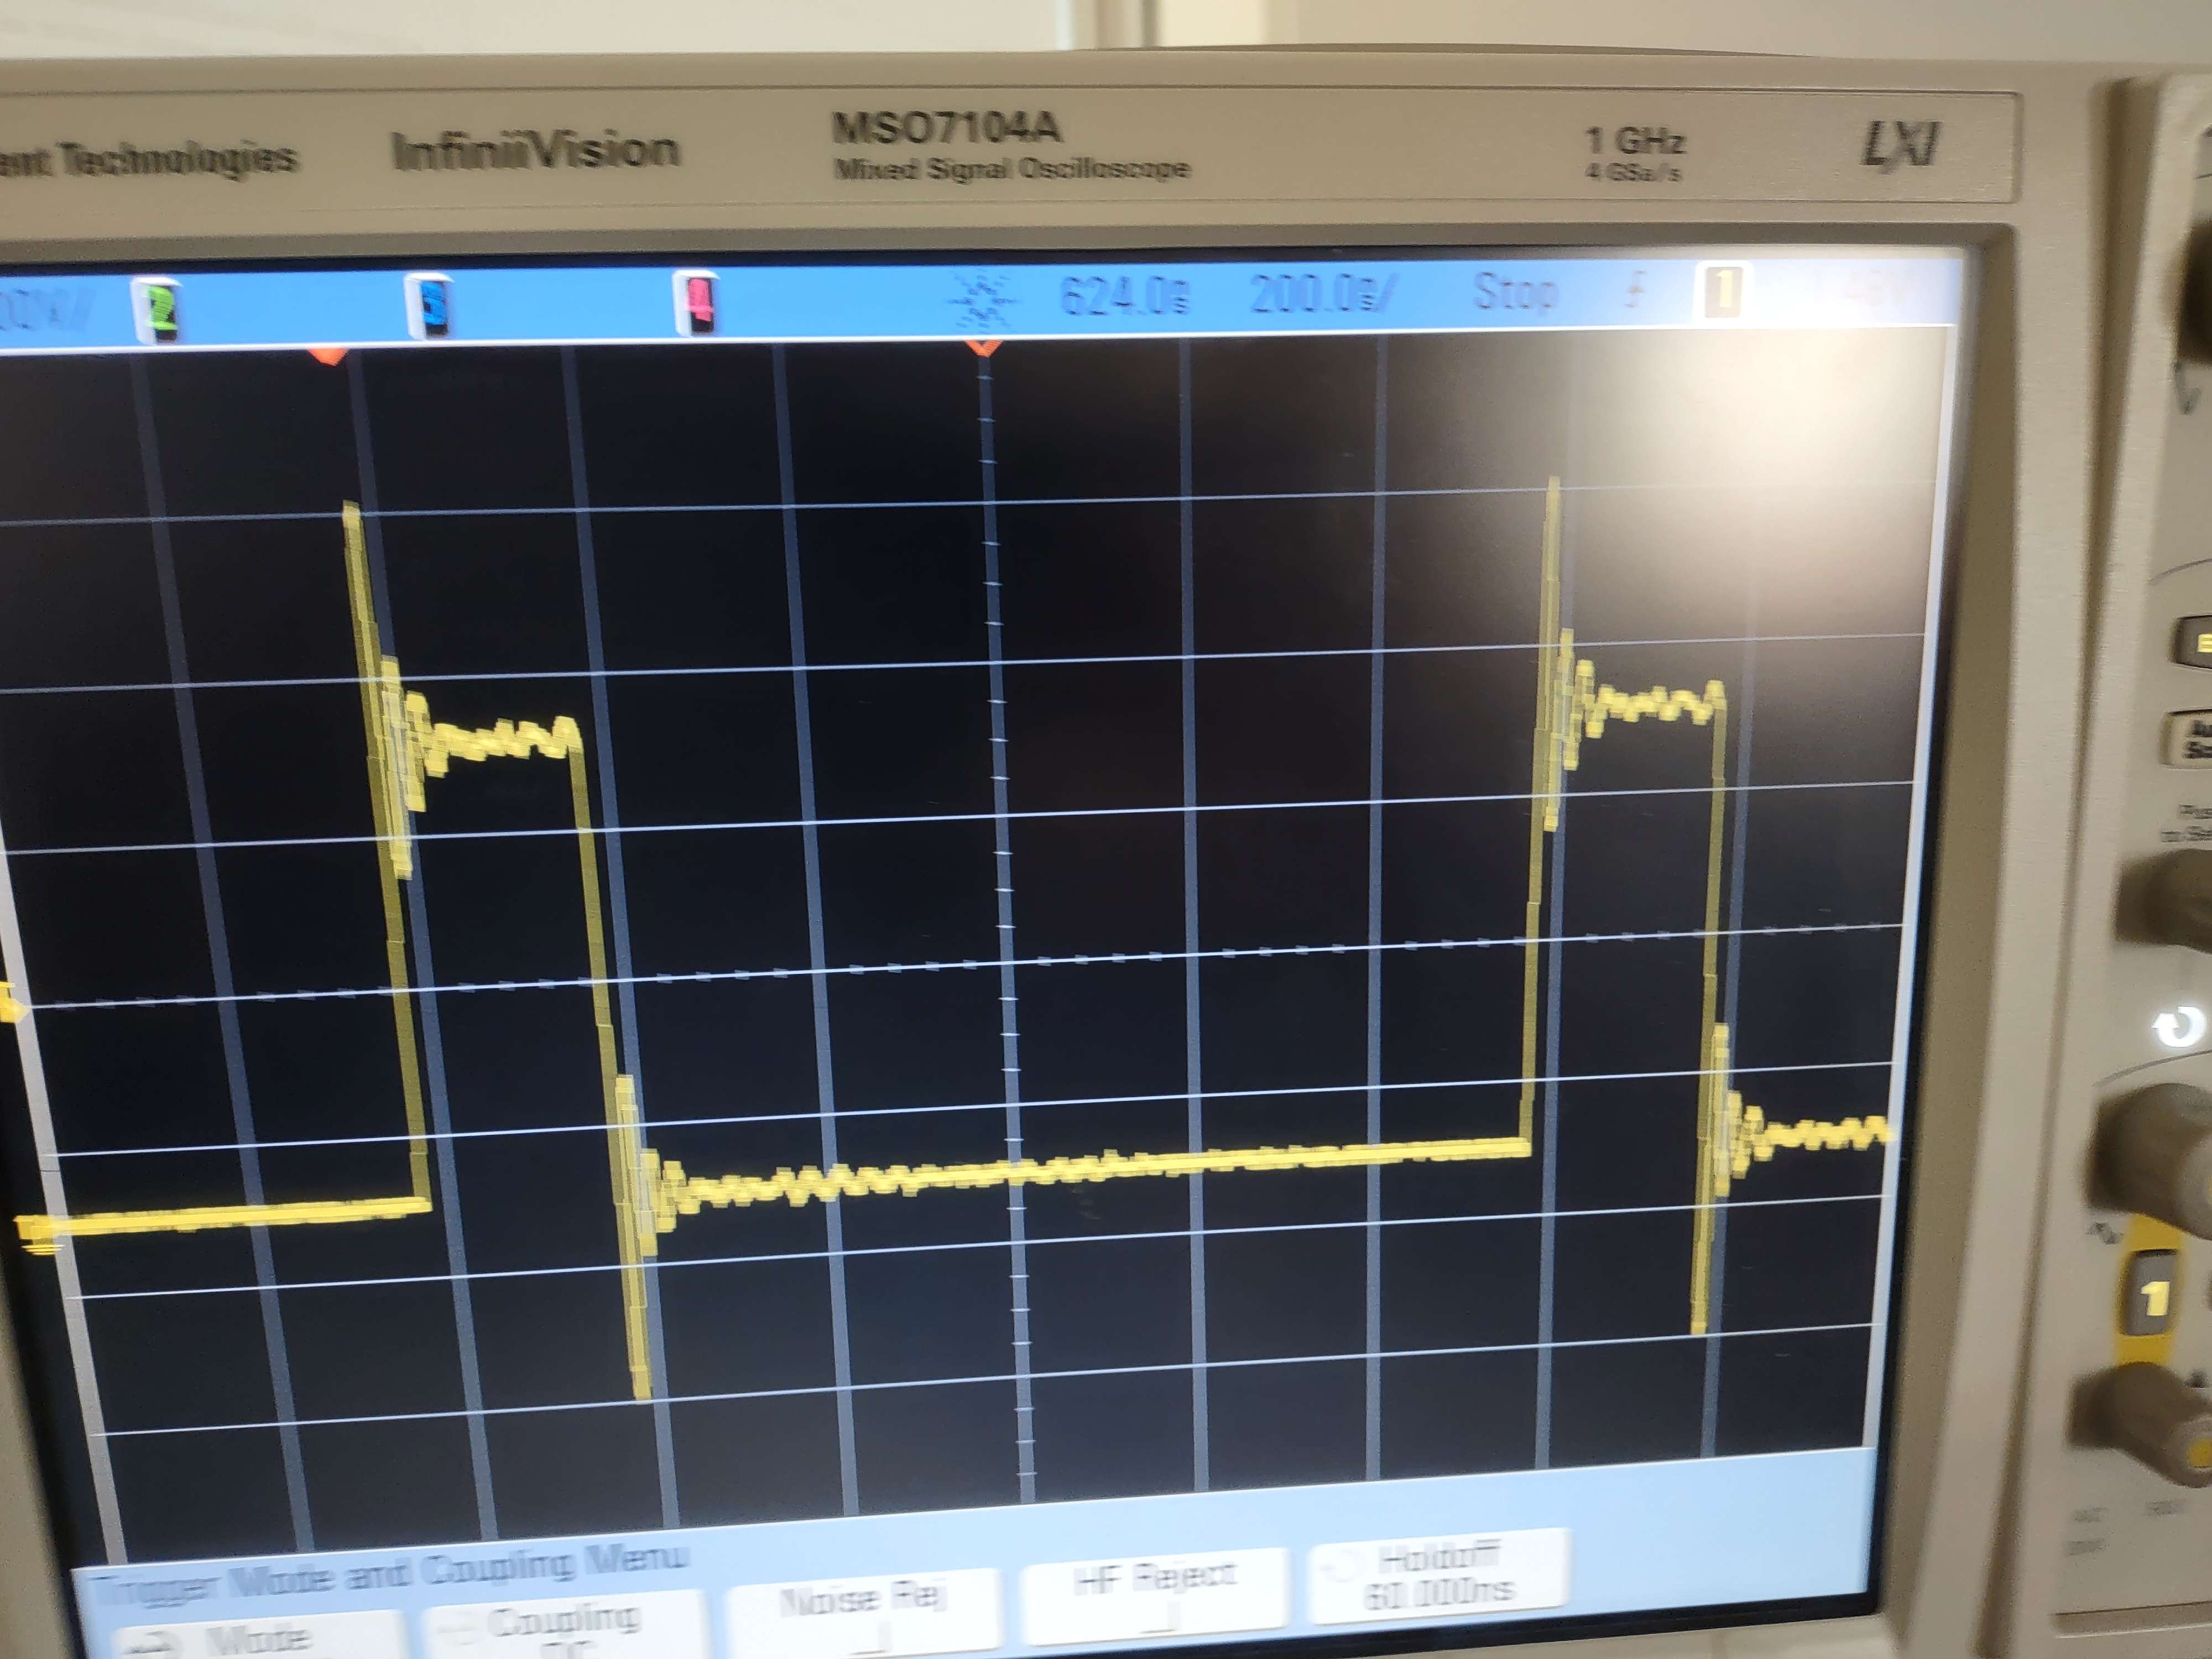
\includegraphics[width=\textwidth]{text/PraktickaCast/img/trampolina.jpg}
  \end{center}
  \label{Semisemafor-zvonek}
  \caption{Zarušená komunikace s ledkami}
\end{figure}

Tento problém jsem vyřešil doplněním feritu do cesty řídícího signálu, abych utlumil vyšší harmonické složky.

Kvůli servisním zákrokům a konstrukci krytu jsem navíc přidal i další dvě kontaktní plošky pod USB konektor pro možnost přehrání firmwaru bez nutnosti vyjmutí desky.
Výsledné schéma viz \ref{Semisemafor-sch-v2}

\section{Mechanické stavba}
Jedním z podstatných požadavků byla jistá úroveň krytí proti vodě, aby se zařízení dalo používat i za deště.
To nutně neznamená úplnou vodotěsnost, dá se totiž předpokládat, že zařízení bude používáno v poloze, kdy je powerbanka dole a Semisemafor nahoře.
Stačí tedy zajistit těsnost proti stékající vodě jen v jednom směru.

Navíc se během testování objevil ještě požadavek na zpětnou vazbu tlačítka v podobě jeho kliknutí. 
Uživatel totiž musí vědět, že tlačítko skutečně stiskl, na což je mechanická odezva samotného tlačítka ideální.

Po několika iteracích jsem obdržel výsledný vzhled (viz obrázek \ref{Semisemafor-box-render})
\begin{figure}[!h]
  \begin{center}
    \includegraphics[width=0.7\textwidth]{text/PraktickaCast/img/Semisemafor-BOX-render.png}
  \end{center}
  \label{Semisemafor-box-render}
  \caption{Vzhled Semisemaforu}
\end{figure}

Jako technologii výroby jsem zvolil obyčejný FDM 3D tisk.
Původně jsem chtěl použít materiál ASA pro jeho UV odolnost, ale ukázalo se, že jsem nebyl schopen navrhnout mechaniku tak, aby byl výsledek dostatečně voděodolný a zároveň měla tlačítka uspokojivou zpětnou vazbu.
ASA bylo příliš tuhé a cvaknutí mikrospínače příliš utlumilo, aby jej uživatel zaznamenal.
Stejné výsledky jsem měl z PETG, PLA, ABS a několika dalšími materiály. Jediný materiál, u kterého jsem dosáhl uspokojivých výsledků, byl PP (polypropylene).

Problém tisku polypropylenu je jeho tepelná roztažnost, takže pokud se tiskne za běžných teplot má tendenci se při tisku kroutit, což značně zesložiťuje jeho tisk.
Jednou možností by bylo celý tisk provádět při teplotě přes \(120°C\), kde začíná probíhat rekrystalizace a polypropylen se začíná výrazně smršťovat.
Tato možnost ale nese nutnost použití speciální tiskárny, která umožňuje tiskový prostor vytopit na tak vysokou teplotu, a proto byla zvolena méně spolehlivá ale jednodušší metoda.
Použitá metoda je založena na vícemateriálovém tisku, přičemž primární je užitečný tisknutý objekt z polypropylenu a druhý dobře tisknutelný materiál tvoří podpěry a přítlak.
Aby tak bylo možné vytisknout i tvar, který nemá vhodná místa pro umístění přítlaku, musí být opatřen technologickými výstupky, které se po tisku mohou odříznout.

Tiskový model byl tedy doplněn o další objekt zajišťující přítlak a~zároveň i~podpěry.
Výsledek je vidět na obrázku \ref{Semisemafor-box-pritlak}

\begin{figure}[!h]
  \centering
  \includegraphics[width=0.9\textwidth]{text/PraktickaCast/img/Semisemafor-BOX-pritlak.png}
  \label{Semisemafor-box-pritlak}
  \caption{Soustava modelů pro tisk}
\end{figure}

Aby nebylo nutné pouzdro tisknout na více dílů, byla zvolena možnost zatiskávání DPS během tisku.
Pokaždé, když tisk dospěl do správného bodu, pozastavil se, aby bylo možné vložit elektroniku a následně pokračoval.

Kromě elektroniky bylo stejným postupem umisťováno i průhledové "sklíčko".
Aby bylo možné zachovat odolnost proti vodě, bylo toto "sklíčko" také z polypropylenu, aby se během tisku přivařilo k okolní hmotě a vytvořilo tak vodotěsný spoj.

Protože je DPS semaforu oboustranně osazena, byl při zatiskávání ještě jeden problém.
Buď by se totiž DPS vložila zarovnaná s aktuální tiskovou vrstvou plochou substrátu.
To by však znamenalo, že by tisková hlava mohla narazit do nějaké z vystupujících součástek.
Nebo tisknout od horního bodu nejvyšší součástky, což by ale znamenalo, že by elektronika nebyla pevně uchycena.
Tento problém byl vyřešen vložkou, která se před zatištěním přilepí na spodní stranu DPS a srovná ji do roviny.
Vložka navíc umožnila mít dodatečné kontaktní plošky z druhé strany USB, protože bez ní by se tyto plošky vyzkratovali o stínění USB konektoru.
Za tímto účelem byla také deska vyrobena v tloušťce 0.8mm, aby byly tyto dodatečné plošky lépe kryty. 
DPC opatřena vložkou je vidět na obrázku \ref{Semisemafor-vlozka}

\begin{figure}[!h]
  \centering
  \includegraphics[width=0.6\textwidth]{text/PraktickaCast/img/Semisemafor-vlozka.png}
  \label{Semisemafor-vlozka}
  \caption{DPS Semisemaforu opatřena vložkou}
\end{figure}

\begin{figure}[!h]
  \centering
  \includegraphics[width=0.8\textwidth]{text/PraktickaCast/img/Real-Semisemafor.jpg}
  \label{Semisemafor-real}
  \caption{Reálný kus Semisemaforu}
\end{figure}


Aby bylo tlačítko dostatečně měkké, mělo dostatečně silnou odezvu a zároveň bylo odolné vůči vodě.
Zvolil jsem tenkou membránu ze které vede šoupátko k tlačítku.
Při stisku membrány je tak pomocí šoupátka stisknuto i tlačítko.
Zároveň aby nebylo nutné mačkat přímo na místo kde je uchyceno šoupátko a aby se zabránilo možnému sklouznutí šoupátka z tlačítka.
Zesílil jsem střed membrány, takže se z membrány stal takový hmatník po obvodu uchycený k tělu Semisemaforu, jak je vidět na obr \ref{Semisemafor-rez-tlacitky}

\begin{figure}[!h]
  \centering
  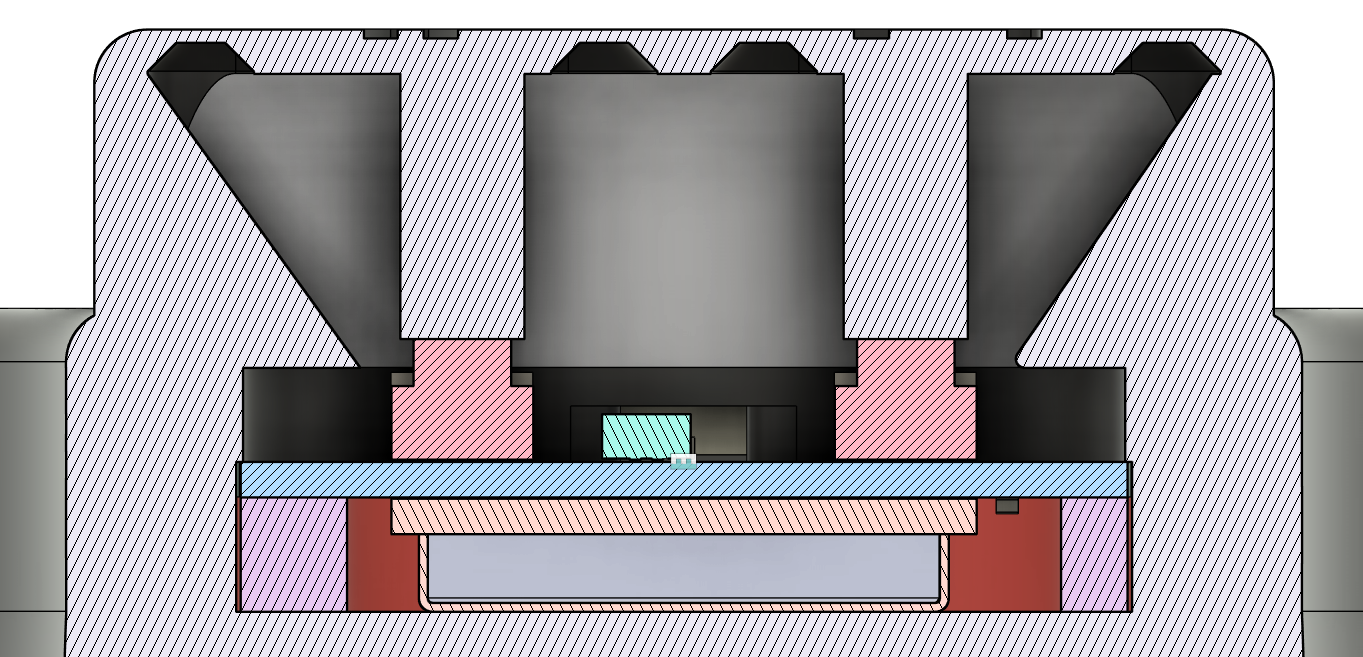
\includegraphics[width=0.8\textwidth]{text/PraktickaCast/img/RezSemaforem.png}
  \label{Semisemafor-rez-tlacitky}
  \caption{Řez tlačítky}
\end{figure}


%%% Vložení souboru 'text/zaver' se závěrem
\chapter*{Závěr}
\phantomsection
\addcontentsline{toc}{chapter}{Závěr}

V~práci je~popsáno několik outdoorových her, které nevyužívají elektroniku a~následně je~rozebrána možnost jejich rozšíření o~elektroniku.
Navíc~je popsána i~jedna hra, která od~základu s~elektronikou počítá.
Na základě těchto her jsou odvozeny požadavky, které jsou na~elektronická zařízení v~hrách kladeny.
Následně byl proveden návrh a~výroba dvou zařízení, která tyto požadavky plní a~je tak možné je~v~outdoorových hrách nasadit.

Jednodušší zařízení je~určeno k~tomu, aby jej hráč nosil sebou, a~jeho cílem je~být dostatečně malé a~levné, aby jej bylo možné používat při hrách ve~velkém počtu.
Využívá mikrokontrloer ESP32C3 \cite{ESP32C3}, dvanáct ledek WS2812B \cite{WS2812B} a~jako zdroj malou powerbanku.

Druhé zařízení je~určeno k~tomu, aby zastoupilo organizátora na~stanovišti a~umožnilo mu~tak zapojení do~hry jiným způsobem.
Toto zařízení tedy už~nemusí být tak malé ani levné, protože se~nepředpokládá nasazení v~tak velkém počtu a~je potřeba, aby bylo dobře viditelné.
Zařízení je~rozděleno na~základní řídící jednotku a~moduly, které jsou k~základní jednotce připojeny pomocí atypicky použitého UARTu.
Nestandardně je~UART použit pro komunikaci jeden s~více, namísto standardního jeden s~jedním (viz podkapitola \ref{sec:ModulovyKonektor}).
To má~za cíl umožnit připojení více modulů k~jedné základní jednotce bez potřeby přeposílání zpráv skrz moduly.
Zařízení má~už vlastní baterii a~elektroniku, která se~stará o~její nabíjení a~chrání ji~proti podbití a~přebití.
Řídícím mikrokontrolerem je~ESP32S3 \cite{ESP32S3} a~také jsou zde využity LED WS2812B tentokrát ve~větším množství.  ~
Významnou částí základní jednotky je~také tlaková plocha (viz kapitoly \ref{popisTlakovky1}, \ref{popisTlakovky2} a~\ref{popisTlakovky3}), která umožňuje hráčům interagovat se~základním zařízením pomocí doteku a~tlaku.

Pro obě zařízení bylo také nutné vytvořit vhodný obal, který dokáže odolat např. dešti, kterému mohou být za~provozu vystaveny.
Zařízení byla také zprovozněna a~ověřena jejich funkce.

%%% Vložení souboru 'text/literatura' se seznamem zdrojů
% \section{Použité zdroje}
% \begin{refsection}
%     \nocite{*}
%     \printbibliography[type=online,title={Online články a dokumenty}]
%     \printbibliography[type=manual,title={Katalogové listy důležitých součástek}]
% \end{refsection}
\clearpage
\section{Použité zdroje}
\nocite{*}
\printbibliography[type=online,title={Online články a dokumenty}, heading=subbibliography]
\printbibliography[type=manual,title={Katalogové listy důležitých součástek}, heading=subbibliography]

%%% Vložení souboru 'text/zkratky' se seznam použitých symbolů, veličin a zkratek
\cleardoublepage
\chapter*{\listofabbrevname}
\phantomsection
\addcontentsline{toc}{chapter}{\listofabbrevname}

\begin{acronym}[KolikMista]

	\acro{AHS}
		{Automatické Herní Stanoviště}

	\acro{LDO}		% název/zkratka
		{Low-dropout regulator - regulátor napětí s nízkým úbytkem}

	\acro{FFC}						% název
		{Flexible Flat Cable - plochý ohební kabel}					% popis

	\acro{DPS}
		{Deska Plošných Spojů}    %CAN, UART, RX, TX, USB, I2C, LDC1614, NFC, LoRa, NB-IoT 
	
	% \acro{PCB}
	% 	{Printed Circuit Board - deska plošných spojů}    %CAN, UART, RX, TX, USB, I2C, LDC1614, NFC, LoRa, NB-IoT 

	\acro{FDM}
	{Fused Deposition Modeling}% - 3D tisková technologie využívající tavení tiskové struny}

	\acro{IMU}
	{Inertial Measurement Unit - inerciální měřící jednotka}% - 3D tisková technologie využívající tavení tiskové struny}

\end{acronym}


%% Začátek příloh
\appendix

%% Vysázení seznamu příloh
% (vynechejte, pokud máte dvě nebo méně příloh)
% \listofappendices

%% Vložení souboru 'text/prilohy' s přílohami
% Obvykle je přítomen alespoň popis co najdeme na přiloženém médiu
\chapter{Schémata AHS}
\label{AHS-sch}
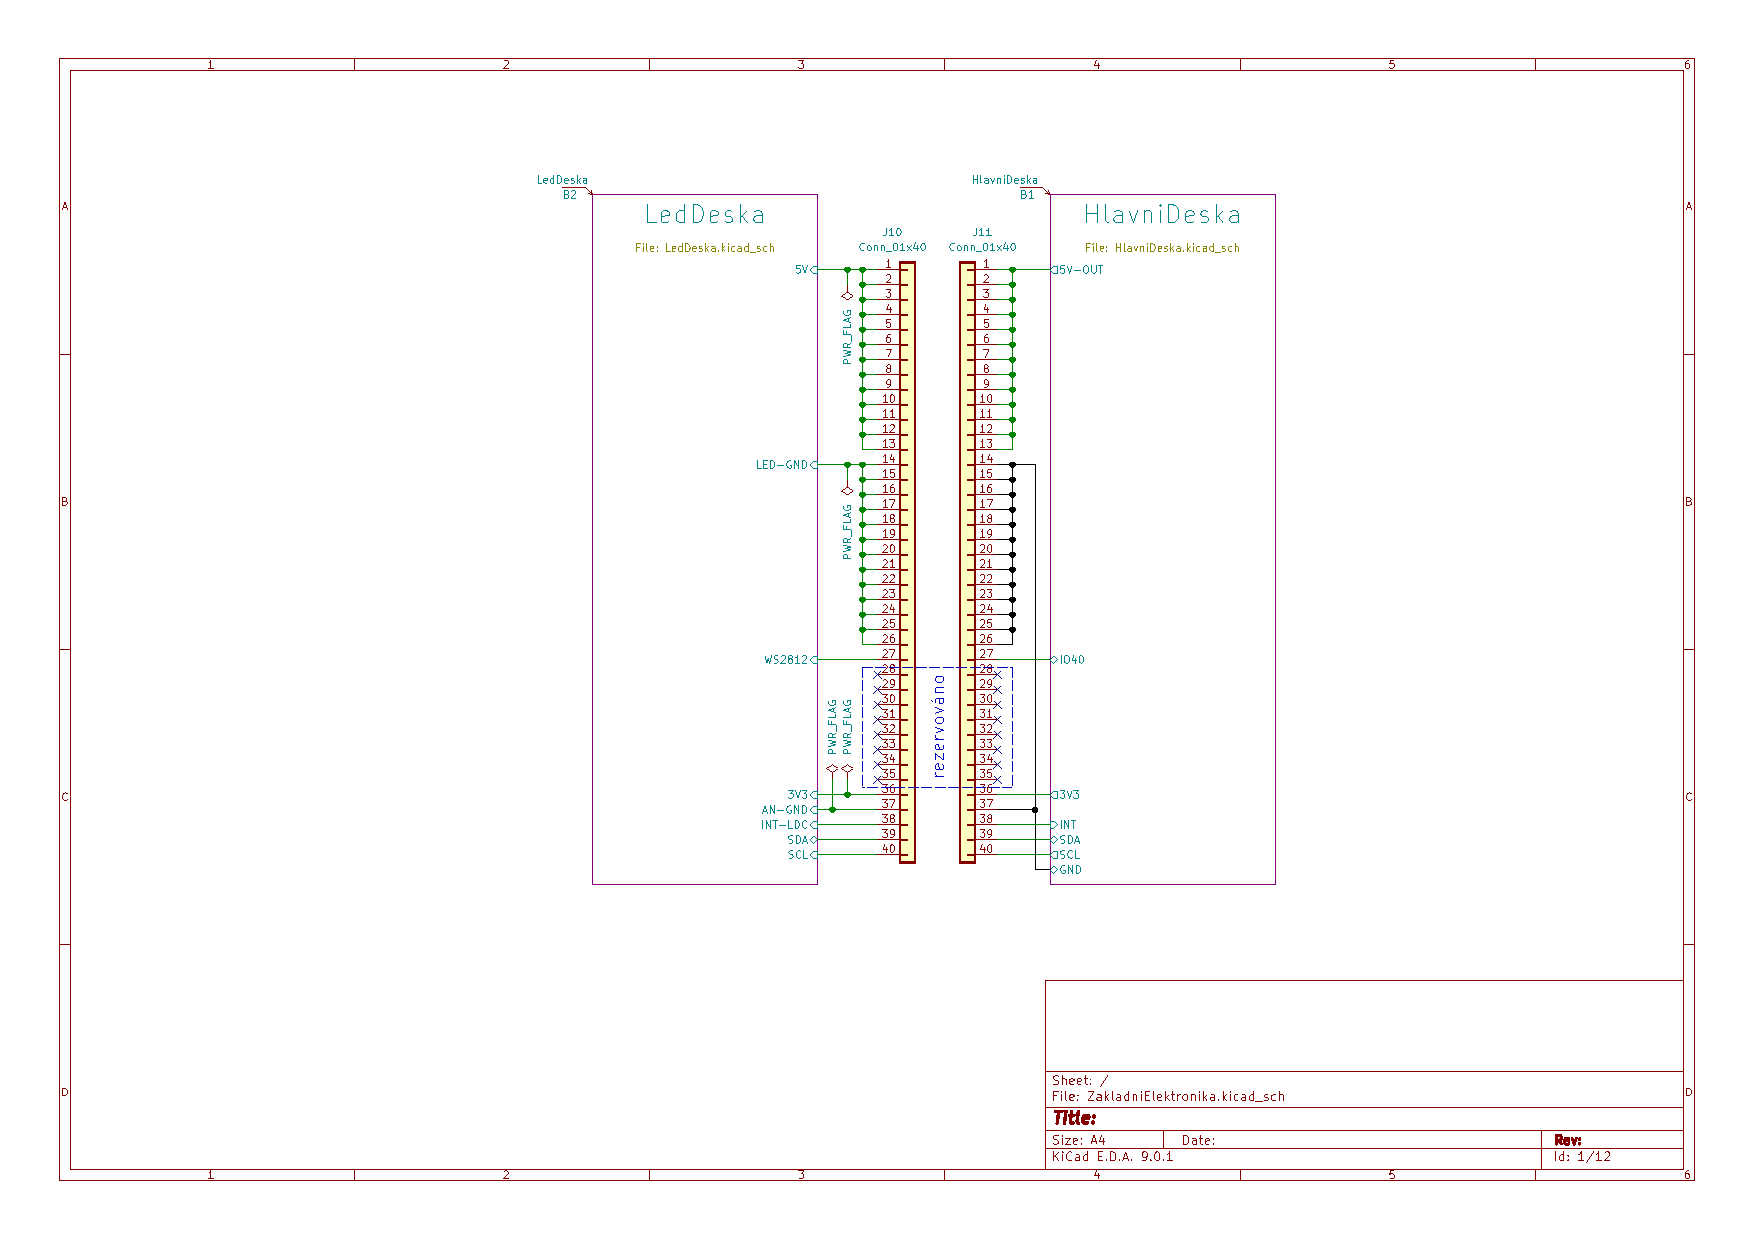
\includepdf[pages=-, angle=90]{text/PraktickaCast/sch/ZakladniElektronika.pdf}

\chapter{Topologie DPS AHS}
\label{AHS-pcb}

\begin{figure}[!h]
	\begin{center}
		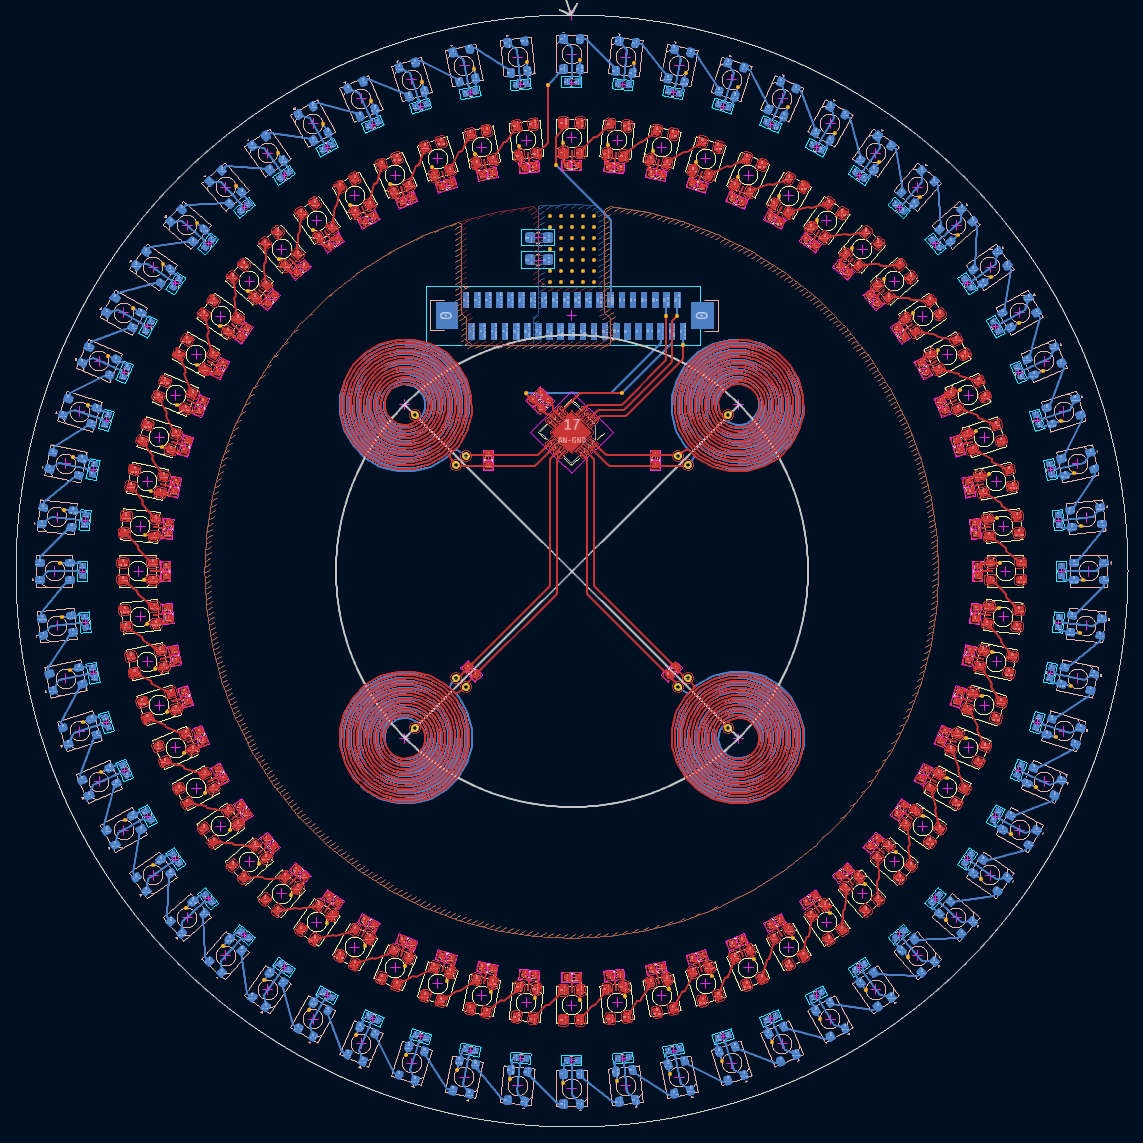
\includegraphics[width=\textwidth]{text/PraktickaCast/img/AHS-DPS-LEDDeska.png}
	\end{center}
	\caption{DPS LED desky AHS}
\end{figure}

\begin{figure}[!h]
	\begin{center}
	  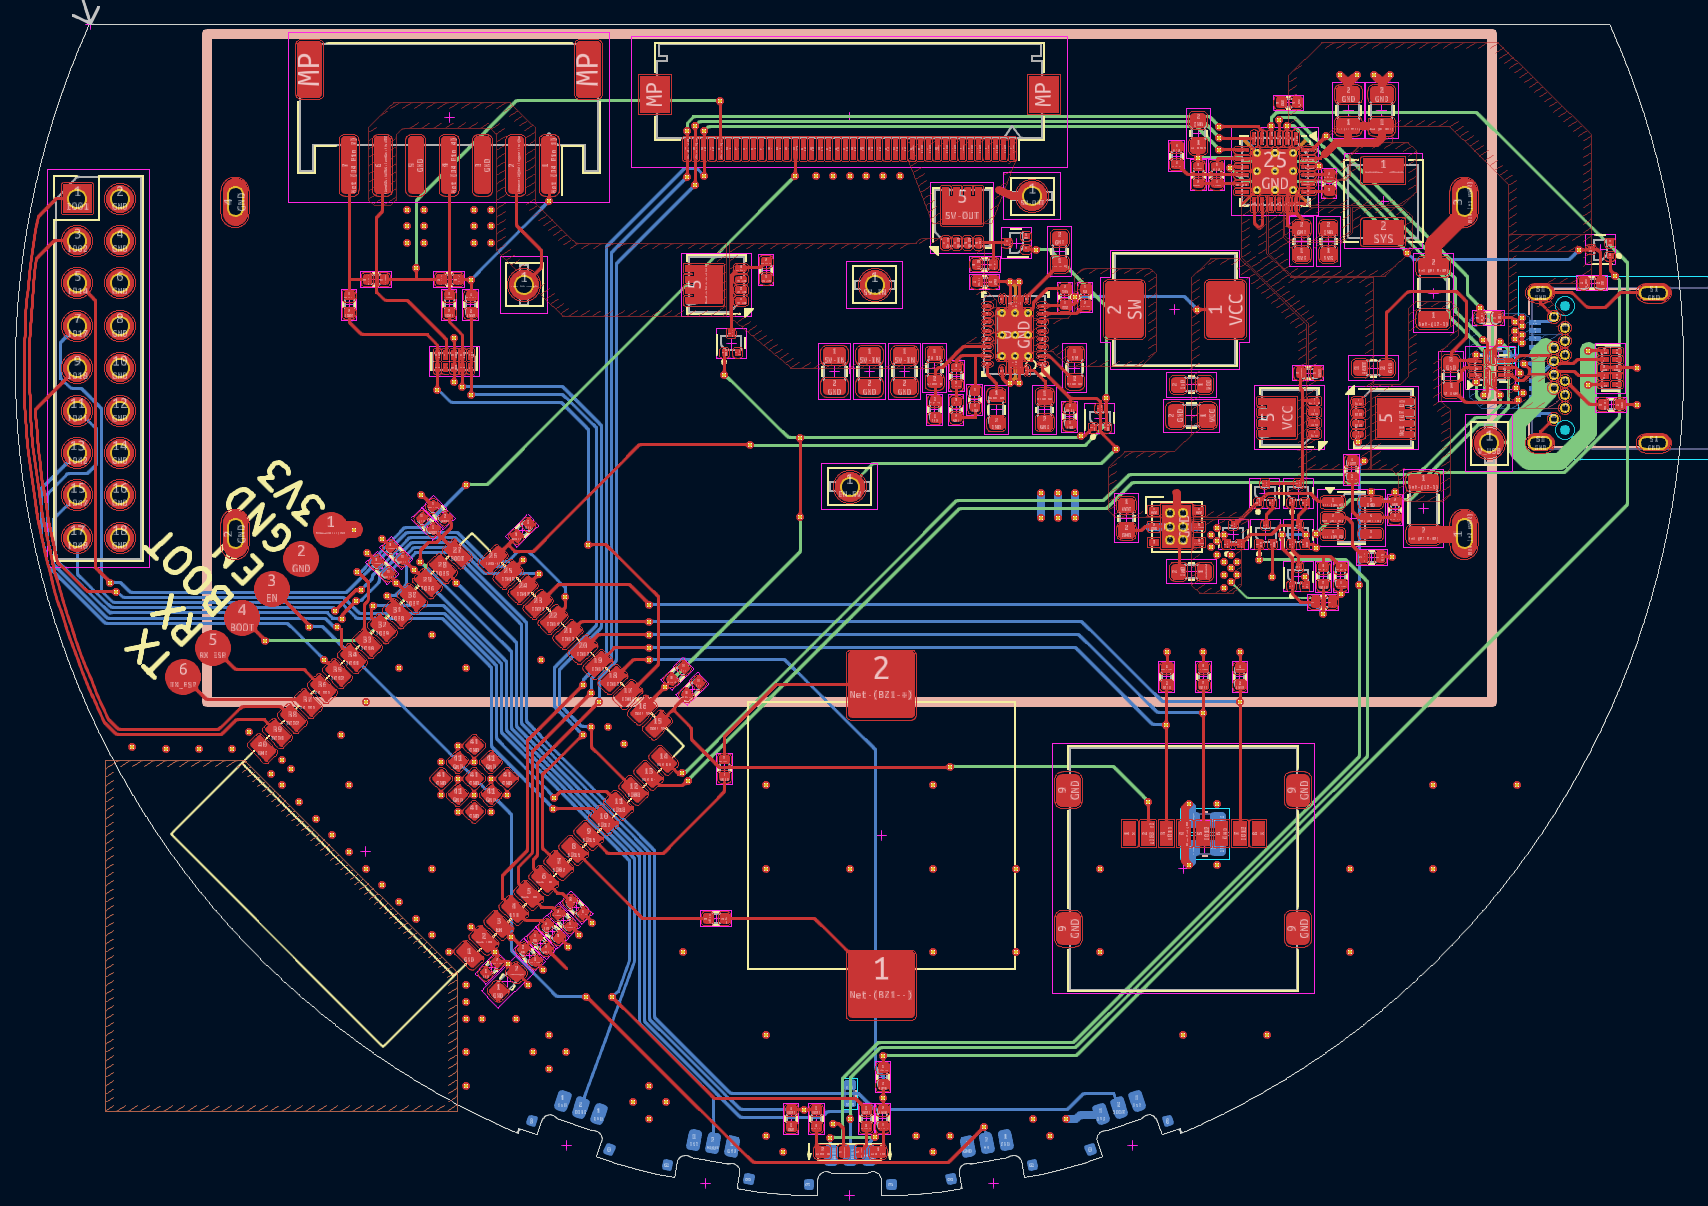
\includegraphics[angle = -90, width=\textwidth]{text/PraktickaCast/img/AHS-DPS-HlavniDeska.png}
	\end{center}
	\caption{DPS hlavní desky AHS}
\end{figure}

\newpage

\chapter{Schémata Semisemaforu}
\section{Původní schéma Semisemaforu}
\includepdf[pages=-, angle=90]{text/PraktickaCast/sch/Semisemafor-V1.0.pdf}

\section{Výsledné schéma Semisemaforu}
\includepdf[pages=-, angle=90]{text/PraktickaCast/sch/Semisemafor-V1.1.pdf}

\chapter{Topologie DPS Semisemaforu}
\begin{figure}[!h]
	\begin{center}
	  \includegraphics[angle = -90, width=0.8\textwidth]{text/PraktickaCast/img/Semisemafor-PCB-V1.png}
	\end{center}
	\caption{Původní DPS Semisemaforu}
	\label{Semisemafor-pcb-v1}
\end{figure}


\end{document}